% Final thing is style report, not article.
\documentclass[12pt,a4paper]{report}

\usepackage{algpseudocode}
\usepackage{color}
\usepackage{amsmath}
\usepackage{tikz}
\usepackage{tabularx}
\usepackage{rotating}
\usepackage{subfigure}
\usepackage{amssymb}
\usepackage{paralist}
\usepackage{multirow}

\newbox\subfigbox             % Create a box to hold the subfigure.
\makeatletter
  \newenvironment{subfloat}% % Create the new environment.
    {\def\caption##1{\gdef\subcapsave{\relax##1}}%
     \let\subcapsave=\@empty % Save the subcaption text.
     \let\sf@oldlabel=\label
     \def\label##1{\xdef\sublabsave{\noexpand\label{##1}}}%
     \let\sublabsave\relax    % Save the label key.
     \setbox\subfigbox\hbox
       \bgroup}%              % Open the box...
      {\egroup                % ... close the box and call \subfigure.
     \let\label=\sf@oldlabel
     \subfigure[\subcapsave]{\box\subfigbox}}%
\makeatother

\usetikzlibrary{arrows,decorations.pathmorphing,decorations.markings,backgrounds,positioning,fit,petri,automata,shapes,petri}

\pgfdeclarelayer{bg}
\pgfsetlayers{bg,main}

% MGK recommends these formatting settings:

% for hard-bound final submission, use:
\setlength{\oddsidemargin}{4.6mm}     % 30 mm left margin - 1 in
% for soft-bound version and techreport, use instead:
%\setlength{\oddsidemargin}{-0.4mm}    % 25 mm left margin - 1 in
\setlength{\evensidemargin}{\oddsidemargin}
\setlength{\topmargin}{-5.4mm}        % 20 mm top margin - 1 in
\setlength{\textwidth}{160mm}         % 20/25 mm right margin
\setlength{\textheight}{247mm}        % 20 mm bottom margin
\setlength{\headheight}{5mm}
\setlength{\headsep}{5mm}
\setlength{\parindent}{0mm}
\setlength{\parskip}{\medskipamount}
\renewcommand\baselinestretch{1.2}
\renewcommand\topfraction{.9}
\renewcommand\textfraction{.1}
\renewcommand\floatpagefraction{.8}

\author{Steven Smith}
\title{Chapter 3}

\begin{document}

\tikzset{BddNode/.style={rectangle,minimum size=6mm}}
\tikzset{BddLeaf/.style={rectangle,minimum size=6mm}}
\tikzset{BddTrue/.style={}}
\tikzset{BddFalse/.style={dotted}}

\tikzset{CfgInstr/.style={rectangle,minimum size=6mm}}
\tikzset{TrueCfgInstr/.style={rectangle,minimum size=6mm,fill=blue!50}}
\tikzset{DupeCfgInstr/.style={rectangle,minimum size=6mm,fill=blue!10}}
\tikzset{NewCfgInstr/.style={rectangle,minimum size=6mm,fill=red!50}}
\tikzset{stateSideEffect/.style={rectangle,draw}}
\tikzset{stateIf/.style={ellipse,draw}}
\tikzset{stateTerminal/.style={ellipse,draw}}
\tikzset{flowChartState/.style={rectangle,draw}}
\tikzset{killEdge/.style={decorate,decoration={snake,segment length=1mm,post length=0.4mm}}}
\tikzset{swungEdge/.style={color=red}}
\tikzset{happensBeforeEdge/.style={dashed}}
\tikzset{ifTrue/.style={}}
\tikzset{ifFalse/.style={dotted}}

\newcommand{\draftonly}[1]{#1}
\newcommand{\editorial}[1]{\draftonly{\textcolor{red}{\footnote{\textcolor{red}{#1}}}}}
\newcommand{\smh}[1]{\draftonly{\textcolor{green}{\footnote{\textcolor{green}{#1}}}}}
\newcommand{\needCite}{\draftonly{\editorial{need cite}}}
\newcommand{\todo}[1]{\draftonly{\textcolor{red}{#1}}}

% Used the first time we introduce a new bit of terminology
\newcommand{\introduction}[1]{\textbf{#1}}
% Backrefs to earlier \introductions.  I'm going to remove the colour
% in the final version, but I want it to be a bit more obvious if I
% have backrefs before introductions in the drafts.
\newcommand{\backref}[1]{\textcolor{purple}{#1}}

\newcommand{\needNewTerm}[1]{\textcolor{blue}{#1}}
\newcommand{\StateMachine}{\needNewTerm{banana}}
\newcommand{\StateMachines}{\needNewTerm{bananas}}
\newcommand{\STateMachine}{\needNewTerm{Banana}}
\newcommand{\STateMachines}{\needNewTerm{Bananas}}
\newcommand{\CrashSummary}{\needNewTerm{strawberry}}
\newcommand{\CrashSummaries}{\needNewTerm{strawberries} }
\newcommand{\implementation}{\needNewTerm{grapefruit}}
\newcommand{\Implementation}{\needNewTerm{Grapefruit}}
\newcommand{\technique}{\needNewTerm{aubergine}}
\newcommand{\Technique}{\needNewTerm{Aubergine}}

\newcommand{\mai}[2]{\mathrm{#1}:\mathrm{#2}}
\newcommand{\happensBeforeEdge}{\leftarrowtail}
\newcommand{\happensBefore}[2]{#1 {\happensBeforeEdge} #2}
\newcommand{\controlEdge}[3]{\mathrm{Control}(\mathrm{#1}:\mathrm{#2} \rightarrow \mathrm{#3})}
\newcommand{\entryExpr}[1]{\mathrm{Entry}(#1)}
\newcommand{\smTmp}[1]{\mathrm{tmp#1}}
\newcommand{\smLoad}[1]{\mathrm{Load}(#1)}
\newcommand{\smBadPtr}[1]{\mathrm{BadPtr}(#1)}

\newcommand{\concatDynTraces}{\oplus}
\newcommand{\interleaveDynTraces}{\otimes}
\newcommand{\survive}{\top}
\newcommand{\crash}{\bot}
\newcommand{\queue}[1]{\{#1\}}
\newcommand{\map}[1]{\{#1\}}
\newcommand{\mapIndex}[2]{#1[#2]}
\newcommand{\state}[1]{\textsc{#1}}

\maketitle
\tableofcontents

\chapter{Deriving and using \StateMachines}

\section{Overview of the {\StateMachine} abstraction}

The core data structure used by {\technique}'s initial analysis phases
is the {\StateMachine}.  This can be viewed as a simplified version of
a fragment of the original program which contains all of the
information relevant to the particular bug under investigation and
very little else.  This makes them far easier to analyse than raw
machine code.  They have a number of important properties:

\begin{itemize}
\item
  They can cross function boundaries, and so can be used to model
  cross-function properties of the program.
\item
  {\STateMachines} are themselves completely deterministic, aiding
  simple analysis, but can contain information from multiple program
  threads, and so can accurately capture all of the threads relevant
  to a particular race, but are themselves completely deterministic,
  aiding simple analysis.  In particular, the {\StateMachine} for a
  particular bug can be used to build the happens-before graph
  necessary for that bug to reproduce (including when that
  happens-before graph is data-dependent).
\item
  {\STateMachines} can incorporate information obtained by the initial
  static and dynamic analysis passes in a reasonably straightforward
  way.
\item
  Control-flow within a {\StateMachine} is not necessarily the same as
  control flow within the original program, and memory accesses within
  a {\StateMachine} do not necessarily correspond to specific memory
  accesses in the original program.  This means that intermediate
  analysis steps have a great deal of flexibility to rewrite
  {\StateMachines} and hence to remove unnecessary information.  On
  the other hand, it also means that translating the results of the
  analysis back from {\StateMachines} to the original program requires
  a some care.  This is discussed in more detail in
  Section~\ref{sect:reproducing_bugs}.
\item
  They can be symbolically executed to determine what initial states
  might lead to the bug, expressed in terms of the program's initial
  state, its happens-before graph, and its control flow.
\item
  Individual {\StateMachines} must complete in a finite, bounded,
  number of operations; equivalently, {\StateMachines} are acyclic and
  finite.  This makes them far easier to analyse, but at the expense
  of somewhat limiting their expressive power.  In the particular case
  of {\technique}, we are only interested in bugs related to fairly
  small fragments of the program (those which should have been
  critical sections, but aren't) and so this is a tolerable
  limitation; it might be more of a concern in other applications.
  Section~\ref{sect:future_work:generalising} briefly discusses some
  possible ways of removing this restriction.
\end{itemize}

{\STateMachines} are in many respects similar to executable program
slices of the original program, with the key difference that, unlike a
program slice, a {\StateMachine} is not expressed in the same language
as the original program.  This is to some extent a forced decision
({\technique} operates on binaries, whereas most program slicing
systems operate on source code; programming languages are not usually
particularly convenient intermediate forms, but machine code is far
worse), but the extra flexibility can sometimes make this more
convenient than more conventional source-level program slices.

A somewhat closer analogy is with the abstract models commonly used in
formal verification systems such as Promela\cite{Holzmann1991}.  The
difference here is in the semantic structure of the program to be
modelled: {\technique} models machine-code programs, and hence has no
knowledge of higher-level constructs such as variables, arrays, or
compound structures, whereas tools like Promela or
SAL\cite{Howard2006} work with source code and hence
(mostly\editorial{But not always; dig up some references.}) assume
that such information is available.  This gives them a great deal of
analytical power, but makes it more difficult for them to model
details of the program which are more apparent in machine code than
source code, and, as already mentioned, these details are often
important when investigating concurrency issues.

\subsection{Semantics of {\StateMachines}}

A {\StateMachine} is, at its core, a simplified version of a fragment
of the program expressed in a simple (non-Turing complete) analysis
language, along with some ancillary structures showing how that
fragment relates to the original program.  Programs in the analysis
language consist of a directed acyclic graph of states, starting from
some designated root state and ending at one of the three terminal
states.  Internal states of the graph are either simple two-way
conditionals or side-effect states representing the program's actions.
An overview of the available state types is given in
Table~\ref{table:state_machine_states}.

It is important to emphasise at this stage that {\StateMachines}
states do not directly correspond to instructions in the original
program: one state might represent several instructions, or a single
instruction might be represented by multiple states.  For instance, an
instruction in a function $f$ might correspond to one state when $f$
is called from $g$ and another when $f$ is called from $h$, and
instructions which are not relevant to the behaviour being
investigated will not have any corresponding states at all.  This
gives {\technique} a great deal of flexibility when simplifying
{\StateMachines}, and hence allows it to remove most irrelevant
information from the {\StateMachine}.

In addition to the graph of states, {\StateMachines} may also have
some temporary variables.  These are simple slots into which the
values of expressions and the results of \state{Load} operations can
be stored.  Temporaries can only store simple values, with no internal
structure, and there is no concept analogous to a pointer to a
temporary\footnote{For {\implementation}, {\StateMachine} temporaries
  are simple 128-bit values, so as to be able to store the contents of
  an XMM register in one temporary, but other choices would be
  possible.}.  It is important to note that {\StateMachine}
temporaries do not necessarily correspond to any particular bit of
program state, and that most program state will not be represented by
any temporary.

\begin{table}
\begin{tabular}{lp{11.3cm}}
Expression & Meaning \\
\hline
$\smTmp{A}$ & The value of {\StateMachine} temporary $A$. \\
$\happensBefore{A}{B}$ & True if event $A$ happens before event $B$, false if $B$ happens before $A$.  See section~\ref{sect:implementation_hacks:hb_ordering} for definition if either $A$ or $B$ does not happen. \\
$\entryExpr{\mai{tid}{instr}}$ & True if thread $tid$ starts with instruction $instr$, and false otherwise. \\
$\controlEdge{tid}{A}{B}$ & True if thread $tid$ executed instruction $B$ immediately after instruction $A$. False if it executed some other instruction after $A$ and undefined if it did not execute $A$ at all.\\
$\smBadPtr{expr}$ & True if $expr$ evaluates to a value which is not a valid pointer.\\
$\smLoad{expr}$ & The initial value of the memory at location $expr$. \\
\end{tabular}
\caption{Types of expressions in the {\StateMachine} expression
  language.  The usual arithmetic operators, such as addition,
  multiplication, bit shift, etc., are also supported, but logical
  operators such as $\wedge$ and $\vee$ are not.}
\label{table:state_machine_exprs}
\end{table}

\begin{landscape}
\begin{table}
\begin{tabular}{lllp{5cm}p{12.8cm}}
\multicolumn{2}{l}{State}       & \multicolumn{2}{l}{Fields} & Meaning \\
\hline
\multicolumn{2}{l}{\state{If}}  & \state{cond} & BBDD        & Conditional branch with two successor states.  Evaluates \state{cond}, branching to one successor if it is true and the other if it is false. \\
\hline
\multicolumn{2}{l}{Terminal states} &          &             & Terminal states.  {\STateMachine} execution finishes when it reaches one of these. \\
 & {\stSurvive}              &              &             & The bug has been avoided. \\
 & {\stCrash}                &              &             & The bug will definitely happen. \\
 & {\stUnreached}            &              &             & A contradiction has been reached; this path through the {\StateMachine} should be ignored. \\
\hline
\multicolumn{2}{l}{Side-effect states}\\
 & \state{Load}                 & \state{addr} & Expression BDD & \multirow{2}{12.8cm}{Load from program memory at address \state{addr} and store the result in {\StateMachine} temporary \state{tmp}.} \\
 &                              & \state{tmp}  & {\STateMachine} temporary \\
 & \state{Store}                & \state{addr} & Expression BDD & \multirow{2}{12.8cm}{Store to program memory.  \state{data} and \state{addr} are evaluated to concrete values and the value of \state{data} stored to the address \state{addr}.} \\
 &                              & \state{data} & Expression BDD \\
 & \state{Copy}                 & \state{data} & Expression BDD & Evaluate an expression and store the result in a {\StateMachine} temporary. \\
 &                              & \state{tmp}  & {\STateMachine} temporary \\
\\
 & \state{ImportRegister}       & \state{tid}  & Thread ID       & \multirow{2}{12.8cm}{Copy the value of register \state{reg} in program thread \state{tid} into {\StateMachine} temporary \state{tmp}.} \\
 &                              & \state{reg}  & Register ID \\
 &                              & \state{tmp}  & {\STateMachine} temporary \\
\\
 & \state{Assert}               & \state{cond} & Boolean BDD     & Note that a given condition is true at a particular point in the {\StateMachine}'s execution. \\
 & $\Phi$                       &              &                 & Implement an SSA $\Phi$ node\cite{cytron1991}. \\
\\
 & {\stStartAtomic}          &              &                 & \multirow{2}{12.8cm}{Mark the start and end of atomic blocks, used to constrain the set of schedules which must be considered; see Section~\ref{sect:using:build_cross_product}.} \\
 & {\stEndAtomic}            \\
\end{tabular}
\caption{Types of {\StateMachine} states.}
\label{table:state_machine_states}
\end{table}
\end{landscape}

\subsection{{\STateMachine} expression language}
\label{sect:sm_expr_language}

Any non-trivial {\StateMachine} will include some expressions over the
original program's state.  These are expressed using an expression
language which is described in Table~\ref{table:state_machine_exprs}.
This language is, for most part, quite conventional, and includes
simple mechanisms for querying the program's behaviour and state and
for obtaining the values of {\StateMachine} temporaries, or for
evaluating simple arithmetic operators.

Note that $\smLoad{}$ expressions always evaluate to the initial value
of the selected memory location, and not to the current value, which
may be different if the {\StateMachine} has executed a \state{Store}
operation.  The only way to access the current contents of memory is
via a \state{Load} side-effect.  This means that $\smLoad{}$ is a pure
function and can be re-ordered freely across side-effecting
operations, simplifying analysis.

This language is missing one important feature: logical connectives
such as $\wedge$ or $\vee$.  These operators are not represented using
the expression language, but are instead encoded into binary decision
diagrams, or BDDs\cite{Brace1990}, which are themselves expressed in
terms of the expression language.  These BDDs allow much more
efficient implementations of many common operations than would be
possible with a scheme based entirely on unconstrained expressions.

\begin{figure}
  \begin{center}
  \begin{tikzpicture}
    \node (x) [BddNode] {$\smTmp{A} = 72$};
    \node (y) [BddNode, below = of x] {$\smLoad{\smTmp{B}} = 9$};
    \node (z) [BddNode, below = of y] {$\smTmp{B} > 912$};
    \node (true) [BddLeaf, below left = of z] {$715$};
    \node (false) [BddLeaf, below right = of z] {$\smTmp{C}$};
    \draw [BddTrue] (x) -- (y);
    \draw [BddFalse] (x.east) to [bend left=30] (false);
    \draw [BddTrue] (y) -- (true);
    \draw [BddFalse] (y) -- (z);
    \draw [BddTrue] (z) -- (true);
    \draw [BddFalse] (z) -- (false);
  \end{tikzpicture}
  \end{center}
  \caption{An example expression BDD.  This can evaluate to either
    $715$ or $\smTmp{C}$, depending on the values of $\smTmp{A}$,
    $\smTmp{B}$ and the initial contents of program memory.}
  \label{fig:derive:example_expr_bdd}
\end{figure}

Two types of BDD used in {\StateMachine} states: expression BDDs and
boolean BDDs.  The difference is that boolean BDDs, or BBDDs, are
constrained to evaluate to a simple boolean, whereas expression BDDs
evaluate to an expression in the expression language.  An example
expression BDD is shown in Figure~\ref{fig:derive:example_expr_bdd}.
This BDD evaluates to $715$ if either $\smTmp{A} \not= 72$ or both
$\smLoad{\smTmp{B}} = 9$ and $\smTmp{B} > 912$, or to $\smTmp{C}$
otherwise.  

The important thing to note here is that both the internal nodes and
the leaves of the BDD are expressions in the expression language,
rather than simple boolean variables or boolean constants.  This means
that expression BDDs can represent complex functions of program state
(they are used, for instance, for the address field of a \state{Load}
state), and do not overly complicate any of the usual BDD manipulation
algorithms.  They do, however, mean that expression and boolean BDDs
are only canonical to the extent that expressions in the expression
language can be canonicalised.  Unfortunately, completely
canonicalising general expressions is impossible\editorial{Cite the
  incompleteness theorem.}, and so while ordinary BDDs are canonical
representations of boolean functions those used by {\technique} are
not.  This lack of canonicalisation can sometimes lead to poor
performance if a single function is represented in many different
forms.  Fortunately, a few very simple canonicalisation rules, such as
sorting the arguments to commutative operators and respecting
transitivity of equality, usually suffice to reduce redundancy to an
acceptable level and avoid the worst performance problems.  These are
discussed further in
Section~\ref{sect:implementation_hacks:bdd_ordering}.

\subsection{Example}
\label{sect:derive:simple_toctou_example}

\begin{figure}
  \subfigure[][Crashing thread]{
    \texttt{
    \begin{tabular}{rlll}
              & \multicolumn{3}{l}{crashing\_thread:} \\
      400694: & mov & global\_ptr, &\%rax\\
      40069b: & test & \%rax, &\%rax \\
      40069e: & je   & \multicolumn{2}{l}{4006ad}\\
      4006a0: & mov  & global\_ptr, & \%rax\\
      4006a7: & movl & \$0x5, & (\%rax)\\
    \end{tabular}
    }
    \label{fig:derive:single_threaded_machine_inp:crashing}
  }
  \subfigure[][Interfering thread]{
    \texttt{
      \begin{tabular}{rlll}
        \\
        \\
        & \multicolumn{3}{l}{interfering\_thread:} \\
        4008fb: & movq & \$0x0, &global\_ptr\\
        \\
        \\
      \end{tabular}
      }
    \label{fig:derive:single_threaded_machine_inp:interfering}
    }
  \caption{Two fragments of machine code which, when run in parallel,
    have a bug.  The {\StateMachines} for these fragment are shown in
    \autoref{fig:derive:single_threaded_machine_both}.}
  \label{fig:derive:single_threaded_machine_inp}
\end{figure}

\begin{figure}
  \subfigure[][Crashing {\StateMachine} generated from the machine
    code in
    Figure~\ref{fig:derive:single_threaded_machine_inp:crashing},
    assuming that the bug to be investigated is a crash at 4006a7.]{
  \begin{tikzpicture}
    \node (l1) at (0,2) [stateSideEffect] {l1: \stLoad{1}{\mathrm{global\_ptr}} };
    \node (l2) [stateIf, below=of l1] {l2: \stIf{\smTmp{1} = 0}};
    \node (l4) [stateSideEffect, below=of l2] {l4: \stLoad{2}{\mathrm{global\_ptr}} };
    \node (l3) [stateTerminal, right= of l4] {l3: \stSurvive };
    \node (l5) [stateIf, below=of l4] {l5: \stIf{\smBadPtr{\smTmp{2}}}};
    \node (l6) [stateTerminal, below=of l5] {l6: \stCrash};
    \draw[->] (l1) -- (l2);
    \draw[->,ifTrue] (l2) -- (l3);
    \draw[->,ifFalse] (l2) -- (l4);
    \draw[->] (l4) -- (l5);
    \draw[->,ifFalse] (l5) -- (l3);
    \draw[->,ifTrue] (l5) -- (l6);
  \end{tikzpicture}\hspace{-20mm}
  \label{fig:derive:single_threaded_machine}
  }
  \subfigure[][Interfering {\StateMachine}, generated from the machine code in Figure~\ref{fig:derive:single_threaded_machine_inp:interfering}.]{
    \begin{tikzpicture}
      \node (l7) [stateSideEffect] {l7: \stStore{0}{\mathrm{global\_ptr}}};
    \end{tikzpicture}
    \label{fig:derive:single_threaded_machine_write}
  }
  \todo{Not the prettiest diagram ever.}
  \caption{}
  \label{fig:derive:single_threaded_machine_both}
\end{figure}

Figure~\ref{fig:derive:single_threaded_machine} shows an example of a
simple single-threaded {\StateMachine}\footnote{This is the crashing
  thread component of the simple\_toctou test discussed in more detail
  in Section~\ref{sect:eval:simple_toctou}.}.  It illustrates a simple
time-of-check, time-of-use race: the program loads from
\verb|global_ptr| twice in quick succession, validating the result of
the first and using the result of the second.  It is straightforward
to read off from this diagram that the program might crash if some
other thread modifies \verb|global_ptr| in between the two loads, and
that it will otherwise survive.  Notice that \verb|4006a7|, the
instruction which crashes, is not itself represented in the
{\StateMachine}: by the time that instruction executes, the program is
either doomed to crash or has definitely avoided the bug, and so that
instruction is irrelevant to determining when and whether the bug can
actually happen.

\begin{sidewaysfigure}
  \begin{tikzpicture}
    \node (lA) [stateIf] { \stIf{\happensBefore{\mai{cfg6}{thread1}}{\mai{cfg8}{thread2}}} };
    \node (lB) [stateSideEffect, below = of lA] { l1: \stLoad{1}{\mathrm{global\_ptr}} };
    \node (lCdummy) [below right = of lA] {};
    \node (lC) [stateSideEffect, right = of lCdummy] {l7: \stStore{0}{\mathrm{global\_ptr}} };
    \node (lD) [stateIf, below = of lB] { l2: \stIf{\smTmp{1} = 0} };
    \node (lE) [stateTerminal, below = of lC] { \stUnreached };
    \node (lF) [stateIf, below left = of lD] {\stIf{\happensBefore{\mai{cfg3}{thread1}}{\mai{cfg8}{thread2}}} };
    \node (lG) [stateTerminal, below right = of lD] {\stSurvive};
    \node (lHdummy) [below right = of lF] {};
    \node (lH) [stateTerminal, right = of lHdummy] {\stUnreached};
    \node (lI) [stateSideEffect, below = of lF] {l7: \stStore{0}{\mathrm{global\_ptr}} };
    \node (lJ) [stateSideEffect, below = of lI] {l4: \stLoad{2}{\mathrm{global\_ptr}} };
    \node (lK) [stateIf, below = of lJ] { l5: \stIf{\smBadPtr{\smTmp{2}}} };
    \node (lL) [stateTerminal, below left = of lK] { \stCrash };
    \node (lM) [stateTerminal, below right = of lK] { \stSurvive };
    \draw[->,ifTrue] (lA) -- (lB);
    \draw[->,ifFalse,draw] (lA) -- (lC);
    \draw[->] (lB) -- (lD);
    \draw[->] (lC) -- (lE);
    \draw[->,ifTrue] (lD) -- (lG);
    \draw[->,ifFalse] (lD) -- (lF);
    \draw[->,ifTrue] (lF) -- (lH);
    \draw[->,ifFalse] (lF) -- (lI);
    \draw[->] (lI) -- (lJ);
    \draw[->] (lJ) -- (lK);
    \draw[->,ifTrue] (lK) -- (lL);
    \draw[->,ifFalse] (lK) -- (lM);
  \end{tikzpicture}
  \caption{Cross-product of the {\StateMachines} shown in
    Figures~\ref{fig:derive:single_threaded_machine}
    and~\ref{fig:derive:single_threaded_machine_write}.}
  \label{fig:derive:cross_thread}
\end{sidewaysfigure}

\begin{figure}
  \begin{center}
  \begin{tikzpicture}
    \node (lA) [stateSideEffect] {\stAssert{0 \not= \smLoad{\mathrm{global\_ptr}} \wedge \happensBefore{\mai{cfg6}{thread1}}{\mai{cfg7}{thread2}}} };
    \node (lB) [stateIf, below = of lA] {\stIf{\happensBefore{\mai{cfg3}{thread1}}{\mai{cfg7}{thread2}}} };
    \node (lC) [stateTerminal, below left = of lB] {\stSurvive};
    \node (lD) [stateTerminal, below right = of lB] {\stCrash};
    \draw [->] (lA) -- (lB);
    \draw [->,ifTrue] (lB) -- (lC);
    \draw [->,ifFalse] (lB) -- (lD);
  \end{tikzpicture}
  \end{center}
  \caption{{\STateMachine} from figure~\ref{fig:derive:cross_thread}
    after {\StateMachine} simplification.}
  \label{fig:derive:cross_thread_opt}
\end{figure}

{\STateMachines} become more interesting when they capture the results
of multiple threads.  Figure~\ref{fig:derive:cross_thread} shows an
example of such a {\StateMachine}.  It is the \gls{crossproduct} of
the {\StateMachines} shown in
Figure~\ref{fig:derive:single_threaded_machine_both}.  Note that even
though the {\StateMachine} completely captures the concurrent
behaviour of the two {\StateMachines}, it is itself completely
deterministic, and hence is relatively easy to simplify.  The result
of these simplifications is shown in
Figure~\ref{fig:derive:cross_thread_opt}.  Simplification is generally
cheaper than symbolic execution, and so this can provide a very
worthwhile performance improvement.

\section{Building the crashing thread's \StateMachine}
\label{sect:derive}

The first step in any of {\technique}'s analyses, once the
\gls{programmodel} has been built, is to build a {\StateMachine}
representing the crashing thread.  Depending on the precise mode of
operation, the amount of information available about the crash will
vary from nothing at all, when looking for a currently-unknown bug, to
a full snapshot of the program's memory at the time of the crash.  The
simplest case is when the only information available is the
instruction pointer at the time of the crash, and so I describe that
first; later sections will explain how to generalise this.

The aim of this phase is to take this crashing instruction pointer and
the \gls{programmodel} and use them build a {\StateMachine}
representing the final \gls{alpha} instructions executed by the
crashing thread.  The approach used has three stages:

\begin{itemize}
\item First, determine which instructions need to be included in the
  {\StateMachine}.  This will be a fragment of the program's control
  flow graph which includes every instruction which the crashing
  thread might have executed in the \gls{alpha} instructions
  immediately prior to crashing, and as few other instructions as
  possible.  This is described in more detail in
  Section~\ref{sect:derive:build_static_cfg}.
\item Next, unroll any loops in that control flow graph fragment such
  that all cyclic paths contain at least \gls{alpha}
  instructions.  At that point, the cycles can be safely broken
  without changing the program's behaviour within the
  \gls{analysiswindow}.  This is described in more detail in
  Section~\ref{sect:derive:handling_loops}.
\item The acyclic \gls{cfg} can then be compiled to produce the
  initial {\StateMachine}.  Each instruction in the \gls{cfg} is
  translated independently and the resulting fragments are then
  stitched back together to form the {\StateMachine}.  This is
  described in Section~\ref{sect:derive:compile_cfg}.
\end{itemize}

The resulting {\StateMachine} captures all of the relevant information
from this thread and can be consumed by the rest of the analysis
framework.

\subsection{Building the crashing thread's static control-flow graph}
\label{sect:derive:build_static_cfg}

\begin{figure}
\begin{algorithmic}[1]
\State $\mathit{depth} \gets 0$
\State $\mathit{pendingAtDepth} \gets \queue{\mathit{targetInstrAddress}}$
\State $\mathit{result} \gets \map{}$
\While{$\mathit{depth} < \alpha$}
  \State $\mathit{pendingAtNextDepth} \gets \queue{}$
  \While{$\neg{}\mathit{empty}(\mathit{pendingAtDepth})$}
    \State $\mathit{currentInstr} \gets \mathit{pop}(\mathit{pendingAtDepth})$
    \If {$\mathit{result} \textrm{ has entry for } \mathit{currentInstr}$}
      \State \textbf{continue}
    \EndIf
    \State $\mathit{current} \gets \text{decode instruction at } \mathit{currentInstr}$
    \State $\mapIndex{\mathit{result}}{\mathit{currentInstr}} \gets \mathit{current}$
    \State $\mathit{predecessors} \gets \text{predecessors of } \mathit{currentInstr}$
    \State Add $\mathit{predecessors}$ to $\mathit{pendingAtNextDepth}$
  \EndWhile
  \State $\mathit{pendingAtDepth} \gets \mathit{pendingAtNextDepth}$
  \State $\mathit{depth} \gets \mathit{depth} + 1$
\EndWhile
\end{algorithmic}
\caption{Building a read-side static control flow graph within a
  single function.}
\label{fig:derive:static_read_cfg_single_function}
\end{figure}

The first step in building the crashing thread's {\StateMachine} is to
find its \gls{cfg}.  The simplest case is that all of the needed
instructions are contained within a single function.  In that case,
the algorithm is as shown in
Figure~\ref{fig:derive:static_read_cfg_single_function}.  This
implements a depth-limited breadth-first search starting at the
crashing instruction and exploring backwards through the program's
control flow.  Note that this can result in a \gls{cfg} with multiple roots.

There is a slight subtlety on line 13, which determines the
predecessors of a given instruction.  This is not always completely
trivial given only a program binary.  {\Technique}'s approach depends
on a combination of static and dynamic analysis.  The full details are
given in Section~\ref{sect:program_model:instr_predecessors}.  For
now, assume that there is some function which maps from an instruction
to the set of instructions which might have executed immediately
before that instruction in a single thread.

\subsection{Handling loops in the crashing thread's CFG}
\label{sect:derive:handling_loops}

There may be loops in the \glspl{cfg} generated by the algorithm in
Section~\ref{sect:derive:build_static_cfg}, but {\technique} requires
that the {\StateMachines} be finite and acyclic.  These loops must
therefore be eliminated, and they must be eliminated in a way which is
guaranteed to preserve all paths of length \gls{alpha} ending at the
instruction being investigated.  The approach {\technique} takes is to
unroll the loops, duplicating instructions as necessary, until every
path from a root of the \gls{cfg} to the target instruction is either free
from cycles or of length greater than \gls{alpha}.  The remaining
cycles can then be eliminated without changing the program's behaviour
within the \gls{analysiswindow}.

\begin{figure}
\begin{tikzpicture}
  [node distance=1 and 0.3]
  \begin{scope}
    \node (A) at (0,2) [CfgInstr] {$A_0$};
    \node (B) [CfgInstr] [below=of A] {$B_0$}; 
    \node (C) [CfgInstr] [below=of B] {$C_0$}; 
    \node (D) [CfgInstr] [below=of C] {$D_0$}; 
    \draw[->] (A) -- (B);
    \draw[->] (B) -- (C);
    \draw[->] (C) -- (D);
    \draw[->] (C.east) to [bend right=90] (B.east) node (edge1) [right] {};
    \begin{pgfonlayer}{bg}
      \node (box1) [fill=black!10,fit=(A) (B) (C) (D) (edge1)] {};
    \end{pgfonlayer}
  \end{scope}
  \begin{scope}[xshift=4cm]
    \node (A) at (0,2) [CfgInstr] {$A_0$};
    \node (B) [CfgInstr] [below=of A] {$B_0$}; 
    \node (C) [CfgInstr] [below=of B] {$C_0$}; 
    \node (D) [CfgInstr] [below=of C] {$D_0$};  
    \node (C') [CfgInstr] [right=of C] {$C_1$};
    \draw[->] (A) -- (B);
    \draw[->] (B) -- (C);
    \draw[->] (C) -- (D);
    \draw[->] (B) to [bend right=10] (C');
    \draw[->] (C') to [bend right=10] (B);
    \begin{pgfonlayer}{bg}
      \node (box2) [fill=black!10,fit=(A) (B) (C) (D) (C')] {};
    \end{pgfonlayer}
  \end{scope}
  \begin{scope}[xshift=8cm]
    \node (A) at (0,2) [CfgInstr] {$A_0$};
    \node (B) [CfgInstr] [below=of A] {$B_0$};
    \node (B') [CfgInstr] [right=of B] {$B_1$};
    \node (C) [CfgInstr] [below=of B] {$C_0$};
    \node (D) [CfgInstr] [below=of C] {$D_0$};
    \node (C') [CfgInstr] [right=of C] {$C_1$};
    \draw[->] (A) -- (B);
    \draw[->] (B) -- (C);
    \draw[->] (C) -- (D);
    \draw[->] (C') -- (B);
    \draw[->] (A) -- (B');
    \draw[->] (B') to [bend right=10] (C');
    \draw[->] (C') to [bend right=10] (B');
    \begin{pgfonlayer}{bg}
      \node (box3) [fill=black!10,fit=(A) (B) (C) (D) (C') (B')] {};
    \end{pgfonlayer}
  \end{scope}
  \begin{scope}[xshift=12cm]
    \node (A) at (0,2) [CfgInstr] {$A_0$};
    \node (B) [CfgInstr] [below=of A] {$B_0$};
    \node (B') [CfgInstr] [right=of B] {$B_1$};
    \node (C) [CfgInstr] [below=of B] {$C_0$};
    \node (C') [CfgInstr] [right=of C] {$C_1$};
    \node (C'') [CfgInstr] [right=of C'] {$C_2$};
    \node (D) [CfgInstr] [below=of C] {$D_0$};
    \draw[->] (A) -- (B);
    \draw[->] (B) -- (C);
    \draw[->] (C) -- (D);
    \draw[->] (C') -- (B);
    \draw[->] (A) -- (B');
    \draw[->] (B') -- (C');
    \draw[->] (C'') to [bend right=10] (B');
    \draw[->] (B') to [bend right=10] (C'');
    \begin{pgfonlayer}{bg}
      \node (box4) [fill=black!10,fit=(A) (B) (C) (D) (C') (B') (C'')] {};
    \end{pgfonlayer}
  \end{scope}
  \draw[->,thick] (box1) -- (box2) node [above,midway] {duplicate $C_0$};
  \draw[->,thick] (box2) -- (box3) node [above,midway] {duplicate $B_0$};
  \draw[->,thick] (box3) -- (box4) node [above,midway] {duplicate $C_1$};
  \draw[->,thick] (box4) -- +(2.5,0) node [above,midway] {...};
\end{tikzpicture}
\caption{A CFG containing a cycle.}
\label{fig:cyclic_cfg}
\end{figure}

\begin{figure}
\begin{center}
\begin{tikzpicture}
  [node distance=1 and 0.3]
  \node (A) at (0,2) [CfgInstr] {$A_0$};
  \node (B) [CfgInstr] [below=of A] {$B_0$};
  \node (B') [CfgInstr] [right=of B] {$B_1$};
  \node (C) [CfgInstr] [below=of B] {$C_0$};
  \node (C') [CfgInstr] [right=of C] {$C_1$};
  \node (C'') [CfgInstr] [above right=of B'] {$C_2$};
  \node (D) [CfgInstr] [below=of C] {$D_0$};
  \draw[->] (A) -- (B);
  \draw[->] (B) -- (C);
  \draw[->] (C) -- (D);
  \draw[->] (C') -- (B);
  \draw[->] (A) -- (B');
  \draw[->] (B') -- (C');
  \draw[->] (C'') -- (B');
  \begin{pgfonlayer}{bg}
    \node (box4) [fill=black!10,fit=(A) (B) (C) (D) (C') (B') (C'')] {};
  \end{pgfonlayer}\smh{Center?}
\end{tikzpicture}
\end{center}
\caption{Fully unrolled version of the CFG in
  Figure~\ref{fig:cyclic_cfg}, preserving all paths of length six or
  fewer instructions.  Note that an additional root has been
  introduced at $C_2$.}
\label{fig:unrolled_cyclic_cfg}
\end{figure}

As an example, consider the \gls{cfg} shown at the left of
Figure~\ref{fig:cyclic_cfg}, which contains a loop between
instructions $B_0$ and $C_0$.  This loop must be removed from the \gls{cfg}
while maintaining all paths which terminate at $D_0$ and which contain
\gls{alpha} or fewer instructions.  The algorithm starts by
performing a depth-first traversal backwards through the graph from
$D_0$ until it finds an edge which closes a cycle.  In this case, that
is the edge from $C_0$ to $B_0$.  {\Technique} will therefore break
this edge by duplicating the instruction at the start of the edge,
$C_0$, along with all of its incoming edges (in this case, just the
$B_0$ to $C_0$ edge).  The $C_0$ to $B_0$ edge can then be redirected
to be from $C_1$ to $B_0$, producing the next diagram in the sequence.
All paths which were possible in the old graph will also be possible
in the new one, if duplicated nodes are treated as semantically
equivalent, and the loop is now one instruction further away from the
target instruction $D_0$.  The process then repeats, moving the cycle
steadily further and further away from $D_0$ until all paths ending of
length \gls{alpha} ending at $D_0$ are acyclic, at which point
the cycle can be safely removed from the graph.

Note that the edge which is modified is the back edge, from $C_0$ to
$B_0$, which points ``away from $D_0$'', and not the forwards edge
from $B_0$ to $C_0$.  Trying to break the $B_0$ to $C_0$ edge would
have moved the cycle away from $A_0$ rather than away from $D_0$,
which would not be helpful.

\begin{figure}
\begin{algorithmic}[1]
  \While {graph is not cycle-free}
     \State $edge \gets \textsc{findEdgeToBeBroken}(targetInstr)$
     \If {$edge$ is at least $\alpha$ instructions from target instruction}
        \State {Erase $edge$ from graph}
     \Else
        \State {$newNode \gets$ duplicate of $edge.source$}
        \For {$i$ incoming edge of $edge.source$}
           \State {Create a new edge from $i.source$ to $newNode$}
        \EndFor
        \State {Replace $edge$ with an edge from $newNode$ to $edge.destination$}
     \EndIf
  \EndWhile
\end{algorithmic}
\caption{Loop unrolling and cycle breaking algorithm.
  \textsc{findEdgeToBeBroken} simply performs a depth-first search of
  the graph backwards from $targetInstr$ and returns the first edge
  which completes a cycle.}
\label{fig:derive:read:unroll_cycle_break}
\end{figure}

The complete algorithm is shown in
Figure~\ref{fig:derive:read:unroll_cycle_break}.  This algorithm is
guaranteed to preserve all paths of length $\alpha$ which end at the
target instruction.  There are only two places in the algorithm which
remove existing edges, so consider each in turn.  The first is the
erasure on line 4.  This can only ever affect edges whose shortest
path to a target is at least $\alpha$ instructions long, and so cannot
eliminate any paths to a target of length $\alpha$, and is therefore
safe.  The other is the replacement step at line 10, which replaces an
edge from $edge.source$ to $edge.destination$ with one from $newNode$
to $edge.destination$.  This is safe provided that every path to
$newNode$ has a matching path to $edge.source$, which is ensured by
duplicating all of $edge.source$'s incoming edges to $newNode$.  At
the same time, no additional paths will be introduced, because every
path to $newNode$ has a matching path to $edge.source$.  As such, the
algorithm correctly preserves all paths of length \gls{alpha},
as desired, and does not introduce any more.

This might appear, on the face of it, to be a rather expensive
algorithm: it must explore every path of length \gls{alpha}
ending at the target instruction, and the number of such paths is
potentially exponential in \gls{alpha}.  This is true, but
there are some important mitigating factors:

\begin{itemize}
\item In practice, most code is not particularly branch-heavy, so that
  relatively few instructions have more than one predecessor and the
  base of the exponential is small.
\item With careful implementation, the constant factor can be made
  small.
\item This is not the only analysis performed by {\technique} which
  has exponential cost in \gls{alpha}.  For instance, later
  phases must determine which memory accesses might alias with which
  other accesses; in the worst case, this might involve considering
  all $2^n$ aliasing pairs individually.
\end{itemize}

The overall result is that, despite having cost $O(n^{\alpha})$, this
phase of the analysis rarely accounts for more than a small percentage
of {\implementation}'s total running time (see
Section~\ref{sect:eval:time_breakdowns} for more details).
  
\subsection{Handling cross-function CFGs.}

\label{sect:derive:cross_function_cfgs}

\todo{This whole subsection needs to be rewritten.}

There is, of course, no guarantee that all of the instructions in the
\gls{analysiswindow} will be contained within a single function, and
if they are not then {\technique} must be able to generate appropriate
cross-function \glspl{cfg}.  It does so by partially inlining
functions as necessary to restore the problem to the single-function
case.  This means that instructions must be labelled by both the
pointer of the instruction itself and also by its inlining context,
which is simply the stack of functions into which it has been
inlined\editorial{Not terribly clear.}.  The only slight complications
are that the inlining context is not necessarily known when \gls{cfg}
exploration starts, and it might be necessary to consider the same
instruction in several contexts.

\todo{That's kind of a stupid way of doing this.  Should only need to
  duplicate instructions when the inlining context matters, which is
  pretty much just when we see both the start and end of the
  function.}

There are two important cases to consider: backing into another
function, where the exploration starts in one function and must be
extended backwards into the end of another one, and backing out of
one, where the exploration starts in one function and must be extended
to include that function's callers.  Backing into a function is
simple: the analysis finds the functions which are to be
called\footnote{There might be more than one function if the
  instruction is a dynamic call.  In that case, the \gls{programmodel}
  is used to find the set of all possibly-called functions and they
  are all treated as possible predecessors; see
  Section~\ref{sect:program_model:instr_predecessors}.}, finds all of
the return instructions in those functions, and treats those as the
predecessor of the current instruction with an appropriately extended
inlining context.

Backing out of a function is more complex.  In this case, the analysis
must consider all possible callers of the target function and inline
the target function into each.  

\todo{As I write this I realise that the way I've done this is really,
  really stupid.  I should probably fix that before writing any more
  about it.}\smh{An example or two would probably help, too.}

Tail calls do not require any particular special handling here.  If
the exploration reaches the start of a function then all branches to
that instruction will be treated as possible predecessors of it,
regardless of whether they come from call instructions or simple
branch instructions.

\subsection[Compiling the \glsentrytext{cfg} to a \StateMachine]{Compiling the \gls{cfg} to a \StateMachine}
\label{sect:derive:compile_cfg}

The algorithm presented so far can build a \gls{cfg} of the
instructions in the \gls{analysiswindow}.  The next step is to compile
that \gls{cfg} to form the initial {\StateMachine}.  The
{\StateMachine} analysis language is powerful enough to make
translating individual instructions in isolation completely
straightforward.  Connecting them together is, however, slightly more
difficult, as the edges in the \gls{cfg} no longer match up
precisely with those in the original program, so that, for instance,
an instruction which would normally have a single successor might have
multiple successors in the \gls{cfg}, or one which would normally
have multiple successors might only have one.  There are three cases
which require special care:

\begin{itemize}
\item
  Some edges will be erased from the \gls{cfg}, so that the
  program can branch from the instruction corresponding to $C_1$ to
  $D_0$ but the \gls{cfg} does not allow that to happen.  These
  are converted to branches to the special {\stUnreached} state,
  reflecting the fact that these paths are of no interest to the rest
  of the analysis.

\item
  Some additional edges will have been introduced which do not
  correspond to anything in the original program.  In the example in
  Figure~\ref{fig:unrolled_cyclic_cfg}, instruction $A_0$ had a single
  successor, $B_0$, in the original program, but has multiple
  successors in the unrolled \gls{cfg}.  Each of the $B_i$
  \gls{cfg} nodes will be represented by a separate
  {\StateMachine} state, but there is no condition on the
  original program's state which can be evaluated at $A_0$
  which could determine which of $B_i$ states the
  {\StateMachine} must execute next.  {\Technique} handles
  these by converting them into \StateMachine-level control
  flow using $\controlEdge{}{}{}$\editorial{Looks a bit ugly like that.} expressions which test the
  program's path through the unrolled \gls{cfg}.  See, for
  instance, state $A_0'$ in
  Figure~\ref{fig:state_machine_for_cyclic_cfg}.

  Note that $\controlEdge{}{}{}$ expressions test control flow within
  the unrolled \gls{cfg} rather than control flow within the
  original program \gls{cfg}.  This can sometimes complicate the design of
  crash enforcers; see Section~\ref{sect:enforce:succ} for more
  details.

\item
  The \gls{cfg} can sometimes have multiple roots, each
  represented by a separate {\StateMachine} state, but the
  {\StateMachine} itself must have a single entry state.  The most
  direct way of handling this would be to build an initial prefix of
  the {\StateMachine} which examines the program state and selects an
  appropriate starting state, but this would be quite awkward.  In
  particular, checking that the calling context is correct would
  require loading a number of stack locations, which would place a
  completely unnecessary additional burden on the alias analysis.
  {\Technique} instead uses special $\entryExpr{}$ expressions which
  are booleans reflecting where the thread entered the \gls{cfg}; see, for
  instance, the start state in
  Figure~\ref{fig:state_machine_for_cyclic_cfg}.

\end{itemize}

As a somewhat unrealistic example, suppose that the \gls{cfg} in
Figure~\ref{fig:cyclic_cfg} had been generated from a program
something like this:

\begin{verbatim}
A: MOV rdx -> rcx
B: LOAD *(rcx) -> rcx
C: JMP_IF_NOT_EQ *(rcx + 8), 0, B
D: STORE $0 -> *(rcx)
\end{verbatim}

The \verb|JMP_IF_NOT_EQ| instruction is supposed to indicate that
\verb|C| loads from the memory at \verb|rcx+8|, jumping to \verb|B| if
it is non-zero and proceeding to \verb|D| otherwise.  This will
produce an unrolled \gls{cfg} as in
Figure~\ref{fig:unrolled_cyclic_cfg}, as already discussed, and a
{\StateMachine} as shown in
Figure~\ref{fig:state_machine_for_cyclic_cfg}.  The generated
{\StateMachine} can then be converted to static single
assignment\needCite{} form and passed to the rest of the analysis.

\begin{figure}
\begin{tikzpicture}
  \node[stateIf,initial above] (l1) {\stIf{\entryExpr{\mai{threadId}{A_0}}}};
  \node[stateSideEffect,below = of l1] (l2) {$A_0$: \state{Copy} $\mathit{rcx} \leftarrow \mathit{rdx}$};
  \node[stateIf,below = of l2] (l3) {$A_0'$: \stIf{\controlEdge{threadId}{A_0}{B_0}}};
  \node[stateSideEffect,below = of l3] (l4) {$B_0$: \state{Load} $\mathit{rcx} \leftarrow \ast(\mathit{rcx})$};
  \node[stateSideEffect,below = of l4] (l5) {$C_0$: \stLoad{}{\mathit{rcx}+8}};
  \node[stateIf,below = of l5] (l6) {\stIf{\smTmp{} = 0}};
  \node[stateIf,below = of l6] (l7) {$D_0$: \stIf{\smBadPtr{\mathit{rcx}}}};
  \node[stateSideEffect,below right = of l3] (l8) {$B_1$: \state{Load} $\mathit{rcx} \leftarrow \ast(\mathit{rcx})$};
  \node[stateSideEffect,below = of l8] (l9) {$C_1$: \stLoad{}{\mathit{rcx}+8}};
  \node[stateIf,below = of l9] (l10) {\stIf{\smTmp{} = 0}};
  \node[stateSideEffect,below right = of l1] (l11) {$C_2$: \stLoad{}{\mathit{rcx}+8}};
  \node[stateIf,right = of l3] (l12) {\stIf{\smTmp{} = 0}};
  \node[stateTerminal,below = of l7] (lBeta) {\stCrash};
  \node[stateTerminal,right = of lBeta] (lGamma) {\stSurvive};
  \node[stateTerminal,right = of lGamma] (lAlpha) {\stUnreached};
  \draw[->,ifTrue] (l1) -- (l2);
  \draw[->,ifFalse] (l1) -- (l11);
  \draw[->] (l2) -- (l3);
  \draw[->,ifFalse] (l3) -- (l8);
  \draw[->,ifTrue] (l3) -- (l4);
  \draw[->] (l4) -- (l5);
  \draw[->] (l5) -- (l6);
  \draw[->,ifFalse] (l6) -- (lAlpha);
  \draw[->,ifTrue] (l6) -- (l7);
  \draw[->,ifFalse] (l7) -- (lGamma);
  \draw[->,ifTrue] (l7) -- (lBeta);
  \draw[->] (l8) -- (l9);
  \draw[->] (l9) -- (l10);
  \draw[->,ifTrue] (l10) -- (lAlpha);
  \draw[->,ifFalse] (l10) -- (l4);
  \draw[->] (l11) -- (l12);
  \draw[->,ifTrue] (l12.east) to [bend left=45] (lAlpha);
  \draw[->,ifFalse] (l12) -- (l8);
\end{tikzpicture}
\caption{{\STateMachine} generated from the CFG shown in
  Figure~\ref{fig:cyclic_cfg}.}
\label{fig:state_machine_for_cyclic_cfg}
\end{figure}

\subsection{Building the interfering thread's \StateMachines}
\label{sect:derive:write_side}

At this stage, {\technique} has built the crashing thread's
{\StateMachine} for the bug which is to be investigated.  The next
step is to build the interfering thread's {\StateMachine}.  If we did
not care about computational cost, we would now consider every
possible sequence of \gls{alpha} instructions in the program,
convert each to a {\StateMachine}, and consider every possible
interleaving of the crashing thread's {\StateMachine} with each of
these interfering {\StateMachines}.  This would clearly be completely
impractical for all but the most trivial programs.  Fortunately, it is
possible to significantly reduce the set of sequences which must be
considered by using the \gls{programmodel}.

The \gls{programmodel} includes, for each instruction which reads from
memory, a list of all of the instructions which might store to the
same memory location (see
Section~\ref{sect:program_model:dynamic_alias}).  This instructions in
this list are referred to as the \glspl{interferingstore} for the
crashing thread.  We can then immediately reduce the set of sequences
which need to be considered to just those which include some
instruction from the \glspl{interferingstore} set, which is
already a useful reduction.  Two further observations make it possible
to reduce the set of sequences further.

Most obviously, any instructions in the interfering thread after the
last \gls{interferingstore} cannot possible influence the behaviour of
the crashing thread, and so cannot possibly affect whether the program
crashes.  They can therefore be completely discarded.

Beyond that, it is also possible to discard instructions prior to the
first communicating instruction.  A communicating instruction is
either one of the \glspl{interferingstore} or a load operation which
might alias with one of the stores in the \gls{crashingthread}
{\StateMachine}.  Instructions prior to the first communicating
instruction can influence the behaviour of the interfering thread, but
only by restricting the possible values of thread-local state, such as
machine registers or memory locations, when the interfering thread
starts.  In the absence of any such information, {\technique} will
consider all possible starting configurations, and so discarding these
instructions is sound.

On the other hand, it is not always desirable to discard these
instructions, if the restrictions would have provided useful hints to
later phases of the analysis.  For instance, if the bug to be
investigated is a bad pointer dereference, knowing that the value
stored into a shared structure had previously been dereferenced by the
interfering thread, and hence is definitely a valid pointer, is often
useful.  The approach taken by {\implementation} is to first generate
a set of minimal \glspl{cfg} (i.e. ones in which every root is a
communicating instruction) and to then extend them backwards to
include a small amount of additional context, provided that doing so
does not increase the number of paths through the \gls{cfg} or
cause the length of any path to exceed \gls{alpha}.  In other
words, a \gls{cfg} rooted at instruction A will be extended to
include its predecessor instruction B provided that B is A's only
predecessor and provided that the longest path starting at A is at
most $\alpha - 1$ instructions long\editorial{Not sure that's terribly
  clear.  It's also not terribly important, so maybe not actually a
  problem.}.

The procedure for building interfering {\StateMachines} is then a
variant of that used for building crashing ones: find all of the
potentially interfering store instructions, build an acyclic \gls{cfg} which
includes all traces of appropriate length which start with a
communicating instruction and end with an interfering one, potentially
extend it with a small amount of extra context, and then compile the
\gls{cfg} down to a {\StateMachine}.  The details are, however, slightly
different, and I describe them in the next couple of sections.

\subsubsection{Finding interfering stores}

\todo{This is quite redundant with previous subsubsection.}

The first phase of building the interfering {\StateMachines} is to
determine which stores in the program might possibly interfere with
the crashing {\StateMachine}.  As indicated, this is straightforward:
simply take all \state{Load} states in the crashing thread's
{\StateMachine} and compare them to the \gls{programmodel} to
find all of the store instructions which might possibly interfere with
them.

As a minor optimisation, {\implementation} first attempts to remove
\state{Load}s which are only required because of \state{Assert}
states\footnote{This includes \state{Load}s which influence a
  {\StateMachine} control-flow decision if the only difference between
  the two control-flow paths is in their \state{Assert}ions.}.  Such
\state{Load}s tend to be much less interesting than those which
control the {\StateMachines} actual behaviour.  The mechanism for
doing so is simple: remove the \state{Assert}ions from the
{\StateMachine}, simplify the resulting {\StateMachine} as far as
possible, and then only consider \state{Load}s which remain in the
{\StateMachine} when building the interfering stores set.

Note that \state{Store} operations in the crashing {\StateMachine} are
not considered at this stage.  That is because we only need to
consider code in other threads which might cause the
\gls{crashingthread}'s behaviour to change, and a simple write-write
race will not cause such a change.  Of course, if the written location
is subsequently \emph{loaded} by the \gls{crashingthread} then that
might cause the \gls{crashingthread}'s behaviour to change in an
interesting way, but in that case the racing write will be considered
interesting by virtue of aliasing with the load.

\subsubsection{Build interfering thread CFGs}

The input to this phase of the analysis is the set of
\glslink{interferingstore}{interfering} and
\gls{communicatinginstruction}{communicating} instructions, and the
analysis must build a collection of acyclic \glspl{cfg} which cover
all possible paths through the program which start with a
\gls{communicatinginstruction}, end with an \gls{interferingstore},
and contain at most \gls{alpha} instructions.  This is easier than
building the crashing thread's \glspl{cfg} in the sense that both ends
of the \gls{cfg} are ``bounded'' by some well-defined instruction,
whereas the crashing thread's \glspl{cfg} potentially extend
arbitrarily far backwards; it is harder in the sense that the
interfering thread \gls{cfg} builder must also cluster the
instructions, deciding which should be included in a single trace and
which analysed independently, whereas the crashing thread's
\glspl{cfg} concern only a single instruction.  The overall result is
that the interfering thread's \glspl{cfg} tend to be significantly
smaller and easier to analyse than crashing thread ones but the
unrolling algorithm itself is slightly more involved.

The first phase of the algorithm is to build a (possibly) cyclic
fragment of the original program's control flow graph which includes
all instructions which might possibly be included in one of the final
traces.  This is simple: starting from each potentially communicating
instruction, {\technique} explores forwards for \gls{alpha}
instructions, merges the resulting \gls{cfg} fragments, and then discards
any instructions which cannot reach a potentially interfering store
within \gls{alpha} instructions.  These \gls{cfg} fragments may cross
function boundaries; the details are the same as those for the
crashing thread's \glspl{cfg} in most important respects, and I do not repeat
them here.

The next step is to remove the cycles from the \gls{cfg}.  As with crashing
thread \glspl{cfg}, this is accomplished by duplicating nodes so as to unroll
loops until any path which uses the loop more than once must be longer
than \gls{alpha} instructions, at which point the loop-closing
edges can be safely discarded.  There is, however, one important
difference: in the crashing thread \gls{cfg}, we are interested in any path
which terminates at a specific point, whereas in the interfering
thread \gls{cfg} we need to preserve any path which goes from a
communicating instruction to an interfering store.  This makes it more
difficult to determine when a loop has been unrolled sufficiently, as
it is no longer sufficient to just check the distance to a nominated
target instruction.  {\Technique} solves this problem by labelling
each node in the graph with information about where it might occur in
an interesting path.  The label on an instruction $l$ then consists of
two maps, $\mathit{min\_from}$ and $\mathit{min\_to}$, defined as:

\begin{enumerate}
\item
  $\mathit{min\_from}_l(c)$ is the number of instructions on the
  shortest path from $c$ to $l$, where $c \in C$, the set of all
  communicating instructions.
\item
  $\mathit{min\_to}_l(i)$ is the number of instructions on the
  shortest path from $l$ to $i$, where $i \in I$, the set of all
  interfering stores and their duplicates.
\end{enumerate}

The length of the shortest path from an instruction $c \in C$ to $i
\in I$ which goes via the instruction $l$ is then
$\mathit{min\_from}_l(c) + \mathit{min\_to}_l(i)$, and so it is safe
to discard any instruction $l$ where
\begin{displaymath}
\min_{c \in C}\left(\mathit{min\_from}_l(c)\right) + \min_{i \in I}\left(\mathit{min\_to}_l(i)\right) > \alpha
\end{displaymath}

The asymmetry, taking the distance from only true communicating
instructions but to any duplicate of an interfering store, is perhaps
surprising.  The key observation is that every path which starts at a
duplicated communicating instruction will have a matching path which
starts at the original communicating instruction, and so the ones
which start at the duplicate instruction are redundant\footnote{The
  symmetrical statement is also true: every path which ends in a
  duplicate interfering store has a matching path which ends at a true
  interfering store.  It would therefore also be correct to discard
  paths which end at a duplicate interfering store.  It would not,
  however, be correct to combine the two observations and discard all
  paths which either start with a duplicate communicating instruction
  or end with duplicate interfering stores, as there would then be
  little point in having those duplicates.}.

\begin{figure}
\begin{algorithmic}
  \State {Compute initial labelling of graph}
  \For {$t$ in the set of potentially-relevant stores}
    \While {graph rooted at $t$ is not cycle-free}
       \State $\mathit{edge} \gets \textsc{findEdgeToBeBroken}(t, \{\})$
       \State $\mathit{newLabel} \gets \textsc{combineLabels}(\text{current label of } \mathit{edge}.\mathit{start}, \text{current label of } \mathit{edge}.\mathit{end})$
       \If {$\min_c(\mathit{min\_from}_{\mathit{newLabel}}(c)) + \min_i(\mathit{min\_to}_{\mathit{newLabel}}(i)) > \alpha$}
           \State {remove $\mathit{edge}$}
       \Else
           \State $\mathit{newNode} \gets \text{duplicate } \mathit{edge}.\mathit{end}$
           \For {Edges $e$ leaving $\mathit{edge}.\mathit{end}$}
              \State {Create a new edge from $\mathit{newNode}$ to $e.\mathit{end}$}
           \EndFor
           \State {Set label of $\mathit{newNode}$ to $\mathit{newLabel}$}
           \State {Replace $\mathit{edge}$ with an edge from $\mathit{edge}.\mathit{start}$ to $\mathit{newNode}$}
           \State {Recalculate $\mathit{min\_from}$ for $\mathit{edge}.\mathit{end}$ and its successors, if necessary}
       \EndIf
    \EndWhile
  \EndFor
\end{algorithmic}
\caption{Loop unrolling algorithm for interfering thread CFGs.
  \textsc{findEdgeToBeBroken} and \textsc{combineLabels} are described
  in the text below.}
\label{fig:derive:store_cfg_unroll_alg}
\end{figure}

The complete algorithm is shown in
Figure~\ref{fig:derive:store_cfg_unroll_alg}.  Note that in this
algorithm duplicating a node duplicates its \emph{outgoing} edges,
whereas when building a crashing thread \gls{cfg} the \emph{incoming} edges
are duplicated.  This reflects the fact that interfering thread \glspl{cfg}
are built up forwards from the communicating instructions while crashing
thread \glspl{cfg} are built up backwards from the target instruction.

The algorithm relies on two utility functions:

\begin{itemize}
\item \textsc{findEdgeToBeBroken} just finds the closing edge of some
  cycle in the graph.  The precise choice of edge is not
  important\editorial{I \emph{think} it'll converge on the same thing
    regardless, but it might be nice to show that.  It's certainly
    guaranteed to be correct, but confluence would also be a nice
    property.}.  In {\implementation}'s implementation, this is a
  breadth-first search starting from some arbitrarily chosen root of
  the \gls{cfg} and reporting the first edge to close a cycle.  If the graph
  reachable from that root is acyclic then {\implementation} moves on
  to the next root.  If the sub-graph reachable from every root is
  acyclic then the whole graph is acyclic and nothing more needs to be
  done.
\item \textsc{combineLabels} is also simple, and is responsible for
  computing the label for the new node which would be produced by
  duplicating $\mathit{edge}.\mathit{end}$.  This node will have the
  same outgoing edges as $\mathit{edge}.\mathit{end}$, and so the same
  $min\_to$ label, and a single incoming edge from
  $\mathit{edge}.\mathit{start}$, and hence a $\mathit{min\_from}$
  label which is just $\mathit{edge}.\mathit{start}$'s
  $\mathit{min\_from}$ with one added to every value.
\end{itemize}

The resulting \gls{cfg} can then be compiled to a {\StateMachine} in the
same way as a crashing thread's \gls{cfg} is.  The only major difference is
that the interfering thread's \glspl{cfg} can sometimes contain disjoint
components, in which case each such component is compiled to a
separate {\StateMachine}.

As an example, consider this cyclic \gls{cfg}:

\begin{tikzpicture}
  \node (A) at (0,2) [CommCfgInstr] {$A$};
  \node (B) [CfgInstr, below=of A] {$B$} edge [in=30,out=-30,loop] ();
  \node (C) [InterferingCfgInstr, below=of B] {$C$};
  \draw[->] (A) -- (B);
  \draw[->] (B) -- (C);
  \draw[->] (C) to [bend left=90] (A) node (edge1) [right,midway] {~~~~~~~~};
  \begin{pgfonlayer}{bg}
    \node(box1) [fill=black!10,fit=(A) (B) (C) (edge1)] {};
  \end{pgfonlayer}
  \draw node [right=of box1] {
    \begin{tabular}{lcccc}
             & \multicolumn{1}{c}{$\mathit{min\_to}$} & \multicolumn{2}{c}{$\mathit{min\_from}$} & overall min\\
             & $C$ & $A$ & $C$ \\
      $A$    & 2   & 0   & 1 & 2\\
      $B$    & 1   & 1   & 2 & 2\\
      $C$    & 0   & 2   & 0 & 0\\
    \end{tabular}
  };
\end{tikzpicture}

$A$, in blue, is a communicating instruction and $C$, in green, is an
interfering instruction.  The overall min column is the minimum
$\mathit{min\_to}$ value plus the minimum $\mathit{min\_from}$ one; it
gives the number of edges on the shortest path involving a given node
which starts at a true interfering instruction and ends at any
interfering instruction, whether true or a duplicate.  Assume, for the
purposes of the example, that \gls{alpha} is five.  A
depth-first search starting at $A$ will find the cycle from $B$ back
to itself and attempt to break that cycle by duplicating $B$.  The
resulting graph will look like this:

\begin{tikzpicture}
  \node (A) at (0,2) [CommCfgInstr] {$A$};
  \node (B) [CfgInstr, below=of A] {$B$} edge [in=210,out=150,loop,killEdge] ();
  \node (B1) [NewCfgInstr, right=of B] {$B_1$};
  \node (C) [InterferingCfgInstr, below=of B] {$C$};
  \draw[->] (A) -- (B);
  \draw[->] (B) -- (C);
  \draw[->] (B) to [bend left=10] (B1);
  \draw[->,swungEdge] (B1) to [bend left=10] (B);
  \draw[->] (B1) -- (C);
  \draw[->] (C) to [bend left=90] (A) node (edge1) [right,midway] {~~~~~~~~};
  \begin{pgfonlayer}{bg}
    \node(box1) [fill=black!10,fit=(A) (B) (B1) (C) (edge1)] {};
  \end{pgfonlayer}
  \draw node [right=of box1] {
    \begin{tabular}{lcccc}
            & \multicolumn{1}{l}{$\mathit{min\_to}$} & \multicolumn{2}{l}{$\mathit{min\_from}$} & overall min\\
            & $C$ & $A$ & $C$ \\
      $A$   & 2   & 0   & 1 & 2\\
      $B$   & 1   & 1   & 2 & 2\\
      $B_1$ & 1   & 2   & 3 & 3\\
      $C$   & 0   & 2   & 0 & 0\\
    \end{tabular}
  };
\end{tikzpicture}

New nodes are shown in red, as is the edge which is modified, and
edges which have been removed are shown crossed through.  Notice that
whereas the shortest cyclic path starting at $A$ was previously
$A$,$B$,$B$, of length 3, it is now $A$, $B$, $B_1$, $B$, of length 4.
Suppose that the next depth-first iteration discovers the edge from
$C$ to $A$.  The algorithm will then break this edge by duplicating
$A$:

\begin{tikzpicture}
  \node (A) at (0,2) [CommCfgInstr] {$A$};
  \node (B) [CfgInstr, below=of A] {$B$};
  \node (B1) [CfgInstr, right=of B] {$B_1$};
  \node (C) [InterferingCfgInstr, below=of B] {$C$};
  \node (A1) [NewCfgInstr,right=of C] {$A_1$};
  \draw[->] (A) -- (B);
  \draw[->,swungEdge] (A1) -- (B);
  \draw[->] (B) -- (C);
  \draw[->] (B) to [bend left=10] (B1);
  \draw[->] (B1) -- (C);
  \draw[->] (B1) to [bend left=10] (B);
  \draw[->] (C) -- (A1);
  \draw[->,killEdge] (C) to [bend left=90] (A) node (edge1) [right,midway] {~~~~~~~~};
  \begin{pgfonlayer}{bg}
    \node(box1) [fill=black!10,fit=(A) (B) (B1) (C) (edge1)] {};
  \end{pgfonlayer}
  \draw node [right=of box1] {
    \begin{tabular}{lcccc}
      labels & \multicolumn{1}{l}{$\mathit{min\_to}$} & \multicolumn{2}{l}{$\mathit{min\_from}$} & overall min\\
            & $C$ & $A$ & $C$\\
      $A$   & 2   & 0   & $\infty$ & 2\\
      $A_1$ & 2   & 3   & 1        & 3\\
      $B$   & 1   & 1   & 2        & 2\\
      $B_1$ & 1   & 2   & 3        & 3\\
      $C$   & 0   & 2   & 0        & 0\\
    \end{tabular}
  };
\end{tikzpicture}

Suppose it now selects the $B_1$ to $B$ edge as the cycle-completing
edge.  It will then duplicate $B$:

\begin{tikzpicture}
  \node (A) at (0,2) [CommCfgInstr] {$A$};
  \node (B) [CfgInstr, below=of A] {$B$};
  \node (B1) [CfgInstr, right=of B] {$B_1$};
  \node (B2) [NewCfgInstr, right=of B1] {$B_2$};
  \node (C) [InterferingCfgInstr, below=of B] {$C$};
  \node (A1) [DupeCommCfgInstr,right=of C] {$A_1$};
  \draw[->] (A) -- (B);
  \draw[->] (A1) -- (B);
  \draw[->] (B) -- (C);
  \draw[->] (B) to [bend left=10] (B1);
  \draw[->,killEdge] (B1) to [bend left=10] (B);
  \draw[->,swungEdge] (B1) to [bend left=10] (B2);
  \draw[->] (B1) -- (C);
  \draw[->] (B2) to [bend left=10] (B1);
  \draw[->] (B2) -- (C);
  \draw[->] (C) -- (A1);
  \begin{pgfonlayer}{bg}
    \node(box1) [fill=black!10,fit=(A) (A1) (B) (B1) (B2) (C) (edge1)] {};
  \end{pgfonlayer}
  \draw node [right=of box1] {
    \begin{tabular}{lcccc}
            & \multicolumn{1}{l}{$\mathit{min\_to}$} & \multicolumn{2}{l}{$\mathit{min\_from}$} & overall min\\
            & $C$ & $A$ & $C$\\
      $A$   & 2   & 0   & $\infty$ & 2\\
      $A_1$ & 2   & 3 & 1 & 3\\
      $B$   & 1   & 1 & 2 & 2\\
      $B_1$ & 1   & 2 & 3 & 3\\
      $B_2$ & 1   & 3 & 4 & 4\\
      $C$   & 0   & 2 & 0 & 0\\
    \end{tabular}
  };
\end{tikzpicture}

The length of the shortest cyclic path start at $A$ has again
increased, this time from four to five.  Now duplicate $B$ because of
the $A_1$ to $B$ cycle-completing edge:

\begin{tikzpicture}
  \node (A) at (0,2) [CommCfgInstr] {$A$};
  \node (B) [CfgInstr, below=of A] {$B$};
  \node (B1) [CfgInstr, right=of B] {$B_1$};
  \node (B2) [CfgInstr, right=of B1] {$B_2$};
  \node (A1) [DupeCommCfgInstr,right=of C] {$A_1$};
  \node (C) [InterferingCfgInstr, below=of B] {$C$};
  \node (B3) [NewCfgInstr, below=of A1] {$B_3$};
  \draw[->] (A) -- (B);
  \draw[->,killEdge] (A1) -- (B);
  \draw[->,swungEdge] (A1) -- (B3);
  \draw[->] (B) -- (C);
  \draw[->] (B) -- (B1);
  \draw[->] (B1) to [bend left=10] (B2);
  \draw[->] (B1) -- (C);
  \draw[->] (B2) to [bend left=10] (B1);
  \draw[->] (B2) -- (C);
  \draw[->] (B3) -- (C);
  \draw[->] (B3) to [bend right=45] (B1);
  \draw[->] (C) -- (A1);
  \begin{pgfonlayer}{bg}
    \node(box1) [fill=black!10,fit=(A) (A1) (B) (B1) (B2) (B3) (C) (edge1)] {};
  \end{pgfonlayer}
  \draw node [right=of box1] {
    \begin{tabular}{lcccc}
      labels & \multicolumn{1}{l}{$\mathit{min\_to}$} & \multicolumn{2}{l}{$\mathit{min\_from}$} & overall min\\
            & $C$ & $A$ & $C$\\
      $A$   & 2 & 0 & $\infty$ & 2\\
      $A_1$ & 2 & 3 & 1        & 3\\
      $B$   & 1 & 1 & $\infty$ & 2\\
      $B_1$ & 1 & 2 & 3        & 3\\
      $B_2$ & 1 & 3 & 4        & 4\\
      $B_3$ & 1 & 4 & 2        & 3\\
      $C$   & 0 & 2 & 0        & 0\\
    \end{tabular}
  };\smh{overall min hangs over right hand margin}
\end{tikzpicture}

The next cycle-completing edge considered is that from $B_2$ to $B_1$.
In this case, the new label would have an overall minimum of 5,
matching \gls{alpha}, and so there can be no paths through the
new node which start with a communicating instruction and which end at
an interfering store or a duplicate of it, and so the edge is simply
deleted:

\begin{tikzpicture}
  \node (A) at (0,2) [CommCfgInstr] {$A$};
  \node (B) [CfgInstr, below=of A] {$B$};
  \node (B1) [CfgInstr, right=of B] {$B_1$};
  \node (B2) [CfgInstr, right=of B1] {$B_2$};
  \node (A1) [DupeCommCfgInstr,right=of C] {$A_1$};
  \node (C) [InterferingCfgInstr, below=of B] {$C$};
  \node (B3) [CfgInstr, below=of A1] {$B_3$};
  \draw[->] (A) -- (B);
  \draw[->] (A1) -- (B3);
  \draw[->] (B) -- (C);
  \draw[->] (B) -- (B1);
  \draw[->] (B1) to [bend left=10] (B2);
  \draw[->] (B1) -- (C);
  \draw[->] (B2) to [bend left=10] (B1);
  \draw[->,killEdge] (B2) to [bend left=10] (B1);
  \draw[->] (B2) -- (C);
  \draw[->] (B3) -- (C);
  \draw[->] (B3) to [bend right=45] (B1);
  \draw[->] (C) -- (A1);
  \begin{pgfonlayer}{bg}
    \node(box1) [fill=black!10,fit=(A) (A1) (B) (B1) (B2) (B3) (C) (edge1)] {};
  \end{pgfonlayer}
  \draw node [right=of box1] {
    \begin{tabular}{lcccc}
         & \multicolumn{1}{l}{$\mathit{min\_to}$} & \multicolumn{2}{l}{$\mathit{min\_from}$} & overall min\\
         & $C$ & $A$ & $C$\\
      $A$   & 2 & 0 & $\infty$ & 2\\
      $A_1$ & 2 & 3 & 1        & 3\\
      $B$   & 1 & 1 & $\infty$ & 2\\
      $B_1$ & 1 & 2 & 3        & 3\\
      $B_2$ & 1 & 3 & 4        & 4\\
      $B_3$ & 1 & 4 & 2 & 3\\
      $C$  & 0 & 2 & 0        & 0\\
      New label & 1 & 4 & 5 & 5\\
    \end{tabular}
  };
\end{tikzpicture}

This process iterates, removing one cycle-completing edge at a time,
until the graph is completely acyclic:

\begin{tikzpicture}
  \node (A) at (0,2) [CommCfgInstr] {$A$};
  \node (B) [CfgInstr, below=of A] {$B$};
  \node (B1) [CfgInstr, right=of B] {$B_1$};
  \node (B2) [CfgInstr, right=of B1] {$B_2$};
  \node (A1) [DupeCommCfgInstr,right=of C] {$A_1$};
  \node (C) [InterferingCfgInstr, below=of B] {$C$};
  \node (B3) [CfgInstr, below=of A1] {$B_3$};
  \node (C1) [DupeInterferingCfgInstr, below=of B3] {$C_1$};
  \node (B4) [CfgInstr, right=of B3] {$B_4$};
  \draw[->] (A) -- (B);
  \draw[->] (A1) -- (B3);
  \draw[->] (B) -- (C);
  \draw[->] (B) -- (B1);
  \draw[->] (B1) -- (B2);
  \draw[->] (B1) -- (C);
  \draw[->] (B2) -- (C);
  \draw[->] (B3) -- (B4);
  \draw[->] (C) -- (A1);
  \draw[->] (B3) -- (C1);
  \draw[->] (B4) -- (C1);
  \begin{pgfonlayer}{bg}
    \node(box1) [fill=black!10,fit=(A) (A1) (B) (B1) (B2) (B3) (C) (C1) (edge1)] {};
  \end{pgfonlayer}
  \draw node [right=of box1] {
    \begin{tabular}{lccccc}
            & \multicolumn{2}{l}{$\mathit{min\_to}$} & \multicolumn{2}{l}{$\mathit{min\_from}$} & overall min\\
            & $C$ & $C_1$ & $A$ & $C$ \\
      $A$   & 2 & 5 & 0 & $\infty$ & 2\\
      $A_1$ & $\infty$ & 2 & 3 & 1 & 3\\
      $B$   & 1 & 4 & 1 & $\infty$ & 2\\
      $B_1$ & 1 & 4 & 2 & $\infty$ & 3\\
      $B_2$ & 1 & 4 & 3 & $\infty$ & 4\\
      $B_3$ & $\infty$ & 1 & 4 & 2 & 3\\
      $B_4$ & $\infty$ & 1 & 5 & 3 & 4\\
      $C$   & 0 & 3 & 2 & 0 & 0\\
      $C_1$ & $\infty$ & 0 & 5 & 3 & 3\\
    \end{tabular}
  };
\end{tikzpicture}

As desired, the graph has been rendered acyclic while preserving all
paths of length up to five instructions.  As a minor optimisation,
{\implementation} will merge node $B_2$ with $B_4$ and $C_3$ with
$C_2$ before converting the \gls{cfg} to a \StateMachine, as the nodes are
semantically identical and this results in a slightly simpler
\StateMachine.

\smh{This is pretty good, though could be improved somewhat (layout at
  least!)}

\subsection{Stack canonicalisation}

\todo{Need to eval how effective this is.}

The aim of the {\StateMachine} building algorithm is to share work
between different contexts in which the crashing instruction is found
by combining the contexts into a single {\StateMachine}.  This is much
easier if the we can arrange for the stack pointer to always have the
same value at the end of the {\StateMachine}, regardless of where the
{\StateMachine} starts, so that local variable accesses in the
function containing the purported crashing instruction match up
properly\footnote{Of course, this means that stack references near the
  start of the {\StateMachine} will be less likely to match up.  This
  is usually a reasonable trade-off, as all paths through the
  {\StateMachine} end in the same way but might start in completely
  different function contexts.}.  This is not completely trivial if
the starting points are themselves in different functions with
different inlining contexts (see
Section~\ref{sect:derive:cross_function_cfgs}).  This problem can be
solved by examining the generated {\StateMachine} and determining, for
each entry point, how the stack pointer changes between that entry
point and the end and then inserting an opposite change immediately
before the entry point.  Most of the time, the only change to the
stack pointer is adding or subtracting a constant, and so this is
easy.  Otherwise, it fails.  The fact that the stack has been massaged
in this way is recorded in the {\StateMachine} structure so that it
can be undone later when building data-dependent crash enforcers.

\todo{Possibly interesting: this means that once you've converted to
  SSA, the initial generation of the stack pointer refers to its value
  at the \emph{end} of the machine, whereas for every other register
  it refers to the value at the \emph{beginning}.}


\subsection{Extracting a call stack from a core dump}

\todo{I moved this from earlier without rewriting it.  Re-check it.}

The algorithm presented above starts from the assumption that the call
stack and crashing instruction pointer are available.  A core dump
contains all of the necessary information, but not in a convenient
format.  In particular, it is not trivial to extract the call stack
from a core dump without access to compiler debug symbols.  The only
important part of the call stack is the sequence of function calls
which have started but not returned\footnote{Some tools refer to this
  as the backtrace \todo{cite?}.}, and {\technique} has two strategies
for extracting it:

\begin{itemize}
\item
  A static analysis, run on the binary before attempting to analyse
  the core dump, which attempts to map from instruction addresses to
  the offset between the current stack pointer and the address of the
  current function's return address.  When this analysis succeeds it
  makes it easy to determine from the core dump where the function
  will return to, and hence where it was called from, but it will not
  always succeed.  In particular, the \verb|alloca| function can cause
  that offset to change at run-time, and so no static analysis will
  ever succeed.
\item
  An abstract interpreter, which attempts to interpret the program's
  machine code forwards from the point of the crash to determine what
  it would have done if it hadn't crashed.  This proceeds until it
  reaches a \verb|ret| instruction, at which point determining the
  return address is again straightforward.
\end{itemize}

\todo{Need to talk about when you use each, and why you need both.
  Which is potentially awkward, because I've forgotten myself.}

Knowing the contents of the call stack at the time of the crash
effectively tells us what the correct inlining context to use is,
which can then be used to constrain the backing-out-of-function case
discussed above.

\subsection{Finding unknown bugs}
\label{sect:derive:unknown_bugs}

When being used to find previously unknown bugs, {\technique} does not
have the assistance of being told the crashing instruction and call
stack and must instead discover them for itself.  The scheme used is
quite simple: enumerate all of the instructions in a program which
might crash due to a bug of the class being investigated and then
consider each independently in turn.  This is obviously only feasible
if the majority of instructions can be dismissed quickly.
Fortunately, they can be: {\implementation} takes, on average, a few
hundred of milliseconds per instruction on fairly modest hardware,
allowing even large programs with millions of instructions to be
analysed in a few days\editorial{Put some actual numbers in here.}.
Parallelisation would allow this time to be reduced further if
necessary.

Identifying instructions which might crash depends on the type of bug
which is to be investigated, but is generally straightforwards.
{\Implementation} considers three types of crash:

\begin{itemize}
\item Assertion-failure type crashes.  These are caused by the program
  calling a function such as \verb|__assert_fail| or \verb|abort|
  provided by an operating system library.  Finding such functions is
  generally straightforward given the usual dynamic linker
  information, and the initial whole-program static analysis phase can
  then find all callers of those functions.
\item Double free errors.  These are caused by the program calling
  \verb|free| in an incorrect manner.  Again, the dynamic linker
  information allows {\implementation} to quickly find all calls to
  \verb|free| in the program, and these calls are used as the
  potentially-crashing instructions in the program.
\item Bad pointer dereferences.  Any memory-accessing instruction
  could potentially dereference a bad pointer, and so
  {\implementation} simply enumerates all memory accessing
  instructions discovered by the initial static analysis.
\end{itemize}

These potentially-crashing instructions are then considered
independently in turn.  This is, again, potentially rather expensive,
as there can be a very large number of these candidate instructions.
On the other hand, many can be dismissed very quickly (90\% of the
instructions in mysql, for instance, can be analysed in under 250ms;
see Section~\ref{sect:eval:analysis_time} for details), and, because
each instruction is considered independently, the main phase of the
analysis is embarrassingly parallel.  This means that the total cost
of the analysis remains high but tolerable, and that it is likely to
become faster as hardware becomes increasingly parallel, which is
precisely the scenario in which it would be most useful.

\subsection{Handling library functions}
\label{sect:derive:library_functions}

{\Implementation} deals with calls to functions in the operating
system standard library by re-implementing approximations of them as
fragments of {\StateMachine}.  These fragments can then be substituted
into {\StateMachines} as they are being built.  In effect, the library
function is treated as a special sort of instruction, and compiled in
exactly the same way as any other instruction\footnote{In particular,
  memory accesses made by the library function are treated as if they
  were made by the call instruction for the purposes of computing the
  interfering stores set and in the dynamic aliasing analysis.}.  This
is generally straightforwards and I do not give full details here.

\todo{Ugly wording.} The \texttt{free} function is particularly
interesting when {\technique} is being used to investigate double-free
errors.  This function has two possible implementations, illustrated
in Figure~\ref{fig:library_free}.  {\Technique} builds a separate
{\StateMachine} for each call to \texttt{free} which might go wrong
due to freeing a pointer which has already been freed.  The call to
\texttt{free} which is currently being investigated is referred to as
the ``Crashing \texttt{free}'', because it is the one which takes the
place of a crashing instruction, and uses the first implementation.
All other calls to \texttt{free} use the second
implementation\footnote{Note that this includes other calls to
  \texttt{free} in the \gls{crashingthread}.  The last operation
  in the \gls{crashingthread} is the crashing \texttt{free};
  other calls to \texttt{free} in the \gls{crashingthread} will
  be non-crashing.}.

\begin{figure}
  \subfigure[][Crashing \texttt{free}]{
    \begin{tikzpicture}
      \node (l1) [stateSideEffect] {\stLoad{1}{\mathit{last\_free}} };
      \node (l2) [stateIf, below = of l1] {\stIf{\smTmp{1} = \mathit{arg0}} };
      \node (l3) [stateTerminal, below left = of l2] {\stCrash };
      \node (l4) [stateTerminal, below right = of l2] {\stSurvive };
      \draw[->] (l1) -- (l2);
      \draw[->,ifTrue] (l2) -- (l3);
      \draw[->,ifFalse] (l2) -- (l4);
    \end{tikzpicture}
    \label{fig:library_free:crashing}
  }
  \subfigure[][Non-crashing \texttt{free}]{
    \raisebox{17mm}{
    \begin{tikzpicture}
      \node [stateSideEffect] {\stStore{\mathit{arg0}}{\mathit{last\_free}} };
    \end{tikzpicture}
    }
    \label{fig:library_free:non_crashing}
  }

  \caption{{\StateMachine} implementations of the \texttt{free}
    function. $arg0$ is an expression for the platform ABI's first
    argument register; for Linux on AMD64, this is RDI.
    $\mathit{last\_free}$ can be any fixed memory location which is
    not used by the program; {\implementation} uses an address in
    kernel space.}
  \label{fig:library_free}
\end{figure}

The effects of these implementations are hopefully reasonably clear:
non-crashing \texttt{free}s set the $\mathit{last\_free}$ address to
the pointer which was released, and the crashing \texttt{free} then
asserts that the pointer which it releases is not the one which was
most recently released.  This is sufficient to handle the most common
kind of double-free bug (ignoring limitations in the rest of the
analysis).  \todo{But not \emph{all} double-free bugs.  Not sure if I
  need to go into detail of the ones where it doesn't work; they're
  fairly obvious, and it's not like I've ever claimed this works every
  time.}

\subsection{The W isolation property}

\label{sect:derive:w_isolation}

\todo{Wording in this section is quite clunky.  Also, the name is
  perhaps a little obscure.}

As discussed in Section~\ref{sect:intro:overview}, {\technique} is
concerned with bugs in which two threads are simultaneously operating
on the same data structure.  This could sensibly be further restricted
to bugs in which the \gls{interferingthread} is modifying a
structure which the \gls{crashingthread} is reading.  In
particular, there is an interesting class of bugs in which the
\gls{interferingthread} does not load any locations which were
previously stored to by the \gls{crashingthread}.  This is
referred to as the \gls{w-isolation} property.  Assuming that
it always holds makes the analysis somewhat simpler, but at the
expense of excluding some bugs from consideration.  {\Implementation}
can be configured to assume that the property holds, and I present
some experimental results on the effect of this assumption in
Section~\ref{sect:eval:w_isolation}.

Most of the optimisations which depend on the \gls{w-isolation}
property are reasonably obvious, and for the most part amount to
simply restricting the aliasing problem.  The main exception is that
it reduces the set of \glspl{communicatinginstruction} which must be
considered when building the \gls{interferingthread} \glspl{cfg}.  In
particular, with the \gls{w-isolation} assumption, the only possible
communication between the \glslink{crashingthread}{crashing} and
\glslink{interferingthread}{interfering} threads is between a store in
the \gls{interferingthread} and a load in the \gls{crashingthread},
and so the \glspl{communicatinginstruction} set is just the set of
\glspl{interferingstore}.

\section{Generating a verification condition}
\label{sect:using:check_realness}

Previous sections have described how to generate pairs of
{\StateMachines} representing fragments of the program which might
interact in interesting ways when run concurrently.  The next step is
take each of those pairs and, for each, determine whether running the
two {\StateMachines} in parallel might lead to a crash, and if so
determine under what circumstances it might do so.

The core of the approach is to take a pair of {\StateMachines}, one
representing the crashing thread and the other representing the
interfering one, and convert them into a
\gls{verificationcondition}\cite{Floyd1967} using symbolic
execution\cite{King1976}.  This \gls{verificationcondition} is
satisfiable precisely when running the fragments of program
represented by the two {\StateMachines} in parallel might cause to the
bug being investigated to reproduce.  This technique is complete in
the sense that if it reports that the program has no bugs then it
definitely does not have any of the form being investigated, provided
that the dynamic analysis is complete and no part of the analysis
times out.  It is not, however, sound, in the sense that some of the
bugs reported might not actually be reproducible, because it ignores
most of the program's existing synchronisation, and this can lead to a
significant number of false positives.
Section~\ref{sect:reproducing_bugs} describes one possible way of
making it sound, at the expense of a significant loss of completeness.

In addition to the verification condition itself, this phase also
generates an \gls{inferredassumption}\editorial{I should probably be
  citing something for that}: a condition which expresses when the
{\StateMachines} would not predict a crash if run atomically, in
either order.  A potential crash is only reported if both the
\gls{inferredassumption} and the \gls{verificationcondition} might be
true simultaneously.  For instance, it might be that the crashing
thread will dereference a pointer stored in a particular stack
location, regardless of the actions of the interfering thread.  The
inferred assumption will then show that that stack location must
contain a valid pointer, and so {\technique} will not report any
potential crashes which depend on it containing an invalid pointer.
This is consistent with the goal of only reporting concurrency bugs,
and not simply any kind of bug in the program.

\begin{figure}
\begin{centering}
\hfill
\begin{tabular}{p{8cm}l}
Crashing thread:\hfill         & Interfering thread: \\
\\
1: Load $t_0$ from loc1        & 6: Load $t_3$ from loc1 \\
2: Store $t_0$ to loc2         & 7: Store $t_3$ to loc2 \\
\textit{Something complicated} & 8: Store $t_3 + 1$ to loc2 \\
3: Load $t_1$ from loc1        & \\
4: Load $t_2$ from loc2        & \\
5: Crash if $t_1 = t_2$ & \\
\end{tabular}
\hfill
\end{centering}
\caption{Example of threads with mandatory concurrency.}\smh{Centre/space}
\label{fig:mandatory_concurrency1}
\end{figure}

\begin{figure}
\begin{centering}
\hfill
\begin{tabular}{p{8cm}l}
Crashing thread:          & Interfering thread: \\
\\
3: Load $t_1$ from loc1   & 6: Load $t_3$ from loc1 \\
4: Load $t_2$ from loc2   & 7: Store $t_3$ to loc2 \\
5: Crash if $t_1 = t_2$   & 8: Store $t_3 + 1$ to loc2
\end{tabular}
\hfill
\end{centering}
\caption{Truncation of the example in Figure~\ref{fig:mandatory_concurrency1}.}
\label{fig:mandatory_concurrency2}
\end{figure}

\todo{Not convinced that this really belongs here; maybe pull up to
  introduction.}

This rule has one non-obvious implication: the ``quality'' of the
results is not monotonically increasing with $\alpha$.  Consider, for
instance, the example in Figure~\ref{fig:mandatory_concurrency1}.  The
crashing thread copies the contents of loc1 to loc2, performs some
complex local calculation, and then asserts that loc1 and loc2 are no
longer equal.  Meanwhile, the interfering thread sets loc1 and loc2 to
$t_3$, then sets loc2 to $t_3 + 1$.  Running the crashing thread
atomically is guaranteed to lead to a crash, and so the inferred
assumption will be simply $\mathit{false}$ and {\technique} will not
report any candidate bugs from this thread pair.  On the other hand,
if the threads were truncated as shown in
Figure~\ref{fig:mandatory_concurrency2} a candidate bug would be
reported.  The crashing thread will survive when run atomically in
isolation if the initial content of loc1 is not equal to the initial
content of loc2, and will always survive if run after the interfering
thread completes, and so the inferred assumption will be
$\smLoad{\mathit{loc1}} \not= \smLoad{\mathit{loc2}}$.  Starting from
a state which satisfies that assumption and interleaving the two
threads in the order 3, 6, 7, 4, 5\editorial{Diagram?} will result in
a crash, and so {\technique} will generate a candidate bug for the
reduced threads.  The original two threads clearly did contain a
concurrency bug, and so increasing $\alpha$ has caused a real bug to
be omitted from the set of candidate bugs.

Note that this is not, strictly speaking, a problem with {\technique}
itself, but rather an unfortunate property of the class of bug
considered.  As discussed in Section~\ref{sect:intro:overview},
{\technique} only considers bugs which are caused by interleaving
threads which would have been safe if they had run without
interleaving.  The truncated program has a bug of that form but the
full program does not (as running the full crashing thread in
isolation will always crash), and so it is unsurprising that
{\technique} will report a bug in the truncated program but not the
full one.

This is nevertheless an irritating property for {\technique} to have.
Fortunately, one could reasonably expect that this problem is rare in
real programs.  In general, real programs will only contain this type
of bug if the complicated local computation in the crashing thread
takes long enough that the interfering thread will almost certainly
intercede, as otherwise the programmer will find the bug quickly and
eliminate it.  At the same time, {\technique} will rarely be able to
support an \gls{analysiswindow} larger than a few hundred
instructions, and on modern hardware the time taken to run a few
hundred instructions will generally be small relative to scheduler
jitter.  It is therefore highly unlikely that the program will be
written such that the interfering thread runs in that part of the
analysis window with high enough probability to make the bug difficult
for a programmer to isolate and fix.  \todo{Not sure how convincing
  that is.  Argument is basically that this kind of bug is easy to
  find, so won't be present in real programs.}


\subsection{Symbolically executing {\StateMachines}}

\todo{This probably wants re-writing.}

{\Implementation} uses a simple symbolic execution engine to evaluate
{\StateMachines} and determine when they will crash.  The details of
this are fairly standard, and I give only a brief overview
here\editorial{\emph{Should} only give a brief overview; this ended up
  much more detailed than I'd expected.}.  The core data structure
used by the execution engine is a queue of (mostly) symbolic
configurations which the {\StateMachine} might occupy, and the main
operation is to take a state out of this queue, determine what the
{\StateMachine} might do next, and possibly add some additional
configurations to the queue to explore further.  Each configuration
contains:

\begin{itemize}
\item
  A mapping from {\StateMachine} variables to the (symbolic) values of
  those variables.
\item
  A reference to the {\StateMachine}'s current (non-symbolic) state.
\item
  A log of all of the memory stores issued by the {\StateMachine} so
  far.
\item
  The current path constraint.  This is simply the conjunction of
  all of the conditions which are known to be true at this point in
  the execution.
\end{itemize}

The core of the symbolic execution engine is a set of rules for
advancing from one symbolic state to another.  Most of these are
standard (see, for instance, \editorial{cite one of the early KLEE
  papers}) and I give only a brief overview of the most important
parts here\editorial{Already said that I'm going to be brief.}.

\begin{itemize}
\item The symbolic execution engine considers only a single
  {\StateMachine} at a time, even when investigating the parallel
  behaviour of two threads.  Rather than trying to enumerate all
  possible interleavings during symbolic execution, {\technique}
  instead encodes them into special cross-product {\StateMachines};
  see Section~\ref{sect:using:build_cross_product}.

\item The program's memory is represented by the sequence of update
  operations, rather than attempting to maintain separate models for
  particular objects or memory locations.  This is because it is not
  always possible to identify precisely which memory location a
  particular memory accessing operation accesses.  Tracking the entire
  list of operations avoids that issue.

  \state{Store} operations are then very easy to implement by just
  adding them to the memory log.  \state{Load} operations, on the
  other hand, are more expensive, and must walk the entire list of
  memory updates and test for aliasing with each one.

  This is equivalent to treating the whole of memory as a single array
  and then using functional updates, as in McCarthy's theory of
  arrays~\needCite{}.  \todo{Say more.}

\item Aliasing queries are resolved lazily.  This means that if the
  engine must execute a \state{Load} operation and cannot immediately
  determine which \state{Store} operation to use, it does not cause an
  immediate fork of its state, but instead causes the \state{Load} to
  return an expression BDD (see Section~\ref{sect:sm_expr_language})
  describing the aliasing query and selecting the appropriate result.
  \todo{I want to say that's faster, and I genuinely believe that it
    is, but I don't have a great deal of evidence to back it up.}
  \todo{Also, might need a better explanation of that.}  \todo{Need to
    check how novel this is.  I suspect it's been done before.}

\item Memory operations, in addition to their main function of
  accessing memory, are also used to infer that certain pointers are
  definitely valid.  For instance, if the engine executes a
  \state{Load} operation which loads from memory with a location given
  by $\mathit{expr}$ it will conclude that $\mathit{expr}$ is a valid
  pointer and add ${\neg}\smBadPtr{expr}$ to the current path
  constraint.  This means that if {\technique} is investigating a bad
  pointer dereference and it can show that either thread dereferenced
  the pointer prior to the crashing instruction then it can assume
  that the crashing instruction will not crash.

  \todo{Ugly ugly ugly}

\item \todo{Rewrite to a para rather than a bullet point.} The engine
  does not attempt to detect when it revisits a previously visited
  configuration.  This is because revisiting configurations is
  extremely rare, and the minimal amounts of redundant work which
  would be avoided by not doing so cannot justify the costs of
  checking for cycles.  There are several reasons for revisiting being
  rare:

  \begin{itemize}
  \item {\STateMachines} are acyclic, and so any single path through
    the {\StateMachine} will definitely not revisit any
    states\footnote{This is also the property which makes not
      detecting cycles safe: there cannot be any infinite loops in the
      execution engine because every path is guaranteed to be finite,
      and there are a finite, if large, number of paths.}.
  \item {\Technique} applies extensive simplification passes to the
    {\StateMachine} before attempting to symbolically execute it (see
    Section~\ref{sect:simplifying}), and these simplifications have
    the effect of removing redundancy from the {\StateMachines}.
  \item The decision to model memory as a sequence of updates, rather
    than as a collection of objects, means that identifying equal
    states is often difficult.  \todo{That was on my list, but I don't
      remember what it means any more.  Think harder.}
  \end{itemize}
\end{itemize}

\subsection{Deriving the inferred assumption}

\label{sect:derive:inferred_assumption}

The \gls{inferredassumption} is a condition on the program's state
which ensures that the \glslink{crashingthread}{crashing} and
\glslink{interferingthread}{interfering} threads do not crash when run
atomically, in either order.  It has two parts: the \gls{ci-atomic}
constraint, which gives the conditions under which running the
\glslink{crashingthread}{crashing} {\StateMachine} and then the
\glslink{interferingthread}{interfering} {\StateMachine} survives, and
\gls{ic-atomic}, which gives the conditions under which running the
\glslink{interferingthread}{interfering} {\StateMachine} and then the
\glslink{crashingthread}{crashing} one survives.  Each sub-condition
is formed by concatenating the two input {\StateMachines} in the
appropriate order, symbolically executing them, and then taking the
disjunction of all paths which end in the {\stSurvive}
state\footnote{Note, in particular, that paths which end at
  {\stUnreached} are not included in the \gls{inferredassumption}.}.
The \gls{inferredassumption} itself is then formed from the
conjunction of these two sub-constraints.

\todo{Might be worth mentioning that W isolation implies CI atomic ==
  C atomic \&\& I atomic, so we can re-use the computation across
  interfering threads when the crashing thread is the same?}

Concatenating {\StateMachines} is straightforward: simply take the
first {\StateMachine} and replace all of its {\stSurvive} states
with branches to the start of the second {\StateMachine}.

\todo{Bad para break.} One might reasonably ask why building the
composite machine is superior to simply symbolically executing one
{\StateMachine} until it reaches the {\stSurvive} state and then
starting the other {\StateMachine} in the resulting configuration.
This would correctly implement the desired behaviour, and would be
somewhat simpler to implement.  The great advantage of building a
composite {\StateMachine} is that the composite {\StateMachine} can be
simplified using the standard {\StateMachine} simplification passes,
which usually reduces the complexity of symbolic execution by a useful
amount, even when the input {\StateMachines} were themselves
simplified as far as possible.  This is because the composite
{\StateMachine} is ``closed'': it contains all potentially relevant
operations, and so the simplification passes can assume that there are
no potentially interfering operations in another thread.  This gives
the simplification passes far more scope to eliminate memory accesses.
The result is that symbolically executing the simplified composite
{\StateMachine} is almost always much faster than executing the input
{\StateMachines} in turn.

This is a similar argument to that made previously by Khoo et
al\cite{Khoo2010}.  In that work, the authors improved the efficiency
of a symbolic execution engine by combining it with a much simpler and
faster type checking system, producing something with the precision of
a symbolic execution engine and performance similar to the type
checker.  In much the same way, building the composite {\StateMachine}
and simplifying it before symbolic execution starts is far cheaper
than trying to symbolically execute the {\StateMachines} in isolation
and then stitch them together via the end and start symbolic states.
\todo{I really don't have a great deal of evidence for that.}

\todo{I would really like to say at this point that deriving the IC
  atomic constraint is the single most expensive part of the analysis
  pipeline.}

\subsection{Building cross-product {\StateMachines}}
\label{sect:using:build_cross_product}

The symbolic execution engine is only capable of exploring one
{\StateMachine} at a time, and so if cross-thread behaviours are to be
investigated then the two single-threaded {\StateMachines} must be
combined into a single multi-threaded one.  This new {\StateMachine}
must capture the complete behaviour of every possible interaction the
two input {\StateMachines}, so that any possible interleaving of their
states is represented by a path through the combined {\StateMachine}.
The approach used by {\technique} is essentially to take a
cross-product of the two {\StateMachines}.  This is a new
{\StateMachine} whose states correspond to pairs of states in the
input {\StateMachine} and whose transitions correspond to advancing
one or other of the two input {\StateMachines}.

There is a close analogy here with the finite state machine
cross-product operation, which is a new FSM whose states correspond to
pairs of states in the input FSMs and whose transitions correspond to
advancing one or other of the input FSMs.  The important difference is
that, in an FSM cross-product, the two FSMs are independent and cannot
influence each other's behaviour, whereas in a {\StateMachine} cross
product they can do, and those influences are precisely what the cross
product is intended to capture.

There are some important subtleties involved in building the
cross-product {\StateMachine}:

\begin{itemize}
\item The input {\StateMachines} might contain {\stStartAtomic} and
  {\stEndAtomic} blocks, which are intended to indicate that some
  fragment of the {\StateMachine} executes atomically.  It is
  important that the output {\StateMachine} is constructed in a way
  which respects those blocks.
\item There will be many pairs of states in the two input
  {\StateMachines} which cannot interact with each other in any way,
  and so can be re-ordered without changing any interesting behaviour.
  The output {\StateMachine} would ideally be constructed in a way
  which avoids forcing later analyses to consider both orderings.  In
  general, there may be many partial-order redundancies\cite{Alur1997}
  between the two {\StateMachines}, and, for efficiency reasons, we
  would like to remove as many of these as possible as early as
  possible.
\item The \gls{crossproduct} {\StateMachine} is only used to
  investigate cases in which the two input {\StateMachines} are
  interleaved, as the cases where they execute atomically will have
  already been considered in the \gls{inferredassumption}.  The
  \gls{crossproduct} {\StateMachine} should therefore be built in a
  way which excludes paths where the input {\StateMachines} run
  atomically.
\end{itemize}

\begin{figure}
  \begin{displaymath}
    \textsc{configuration} = \left(\begin{array}{rrll}
      \multirow{2}{*}{\bigg\{} & \mathit{crashingState}: & \textsc{{\StateMachine} state}, & \multirow{2}{*}{\bigg\},}\\
                               & \mathit{crashingHasIssued}: & \textsc{Bool}\\
      \multirow{2}{*}{\bigg\{} & \mathit{interferingState}: & \textsc{{\StateMachine} state}, & \multirow{2}{*}{\bigg\},} \\
                               & \mathit{interferingHasIssued}: & \textsc{Bool}\\
      \multicolumn{2}{r}{\mathit{atomic}:} & \multicolumn{2}{l}{\{ \varnothing, \mathit{crashing}, \mathit{interfering} \}}
    \end{array}\right)
  \end{displaymath}
  \caption{\textsc{configuration} type for the cross-product algorithm.}
  \label{fig:cross_product:configuration}
\end{figure}

The algorithm used is actually rather simple.  The core idea is to
identify each state of the output {\StateMachine} with a particular
configuration of the two input {\StateMachines}, where the
configuration contains all of the necessary information about the
concurrent interleaving of the two {\StateMachines} and nothing else.
More concretely, a configuration consists of a field showing which, if
either, of the input {\StateMachines} are currently in atomic blocks,
and, for each input {\StateMachine}, that {\StateMachine}'s current
state and a flag indicating whether it has issued any memory accesses.
The output machine starts in a configuration with neither input
{\StateMachine} in an atomic block, both {\StateMachines} at their
initial state, and, and with neither having issued any memory
accesses.  The algorithm then exhaustively explores every
configuration reachable from this one, building the output
{\StateMachine} as it goes.  The rules for advancing from a
configuration are quite simple, and are best explained by means of an
example.  Consider, for instance, the {\StateMachines} shown in
Figure~\ref{fig:cross_product_input}.  $y$ here is supposed to
indicate some value which is local to the interfering thread
{\StateMachine} and $x$ some global variable in memory.  These produce
the cross-product {\StateMachine} shown in
Figure~\ref{fig:cross_product_output}\footnote{These {\StateMachines}
  have no atomic blocks, and so the state related to atomic blocks is
  not shown.}.  I highlight a couple of the more important features of
this diagram:

\begin{itemize}
\item The {\StateMachine} starts in the configuration (\{$A$,
  {\false}\}, \{$E$, {\false}\}), indicating that the crashing thread
  {\StateMachine} is in state $A$, is not in an atomic block, and has
  not issued any memory accesses, and that the interfering thread
  {\StateMachine} is in state $E$, is not in an atomic block, and has
  not issued any memory accesses.  The first state in the interfering
  thread is an \state{If}, which is always thread-local, and so it is
  able to advance immediately.  The resulting state in the output
  {\StateMachine} is therefore an \state{If} state testing the same
  condition as the input \state{If}.  The successor states in the
  output state are then the starting output state with the interfering
  thread's state updated to reflect the result of the conditional
  test.  In other words, when the condition is true, the output
  {\StateMachine} moves to configuration (\{$A$, {\false}\}, \{$I$,
  {\false}\}), because the interfering thread {\StateMachine} will
  move from state E to state I, and when the condition is false the
  output {\StateMachine} moves to configuration (\{$A$, {\false}\},
  \{$F$, {\false}\}), because the interfering thread {\StateMachine}
  moves from $E$ to $F$.

  There is a slight ambiguity here which occurs if both input
  {\StateMachines} are at purely local states.  In that case,
  {\technique} prefers to advance the {\StateMachine} whose current
  state has the smallest number of successor states, as this tends to
  result in the smallest possible output {\StateMachine}.  When both
  input {\StateMachines} have the same number of successor states it
  advances the crashing thread {\StateMachine}.

\item One of the successors of the initial configuration is (\{$A$,
  {\false}\}, \{$I$, {\false}\}).  The interfering thread
  {\StateMachine} has now reached a terminal state, $I$, without
  either input {\StateMachine} issuing any memory accesses.  This
  indicates that both {\StateMachines} have completed atomically,
  which is not an interesting case to investigate, and so {\technique}
  instantiates this output state as {\stUnreached}.  The later
  analysis phases will therefore not investigate this path.  In
  general, any time one of the input {\StateMachines} reaches a
  terminal state and either input {\StateMachine} has failed to issue
  an access the output state should be {\stUnreached}.

\item In the other successor of the initial state, (\{$A$, {\false}\},
  \{$F$, {\false}\}), both {\StateMachines} have reached a memory
  accessing state.  {\Technique} now looks ahead in both input
  {\StateMachines} to determine whether the accesses might involve
  some cross-{\StateMachine} interaction (see below for more details
  of this process).  In this case, they can interact, and so the
  cross-product algorithm uses a happens-before test
  $\happensBeforeEdge{}$ to consider both possible orderings of the
  accesses.  If $\happensBefore{A}{F}$ then the memory access in state
  $A$ should happen before that in state $F$, and so the output
  {\StateMachine} issues the state A access and moves to configuration
  (\{$B$, {\true}\}, \{$F$, {\false}\}).  Otherwise, $F$ should happen
  before $A$, and so it issues the state $F$ access and moves to
  (\{$A$, {\false}\}, \{$I$, {\true}\}).  Other
  potentially-interfering memory accesses are handled similarly.

\item In the configuration (\{$C$, {\true}\}, \{$I$, {\true}\}),
  the crashing thread {\StateMachine} is at a memory accessing state
  $C$ while the interfering thread {\StateMachine} is at a terminal
  state $I$.  There can therefore be no interaction between the access
  at $C$ and any future accesses issued by the interfering thread, and
  so the output {\StateMachine} can issue the $C$ access without needing
  any further $\happensBeforeEdge$ tests.

\item The $F$ state has been duplicated into two places in the output
  {\StateMachine}.  In this case, this is not actually a problem, but
  if F had been a variable-defining state such as \state{Load} or
  \state{Copy} then this would have broken the SSA form.  {\Technique}
  uses a further post-processing step to restore the SSA invariant,
  introducing additional variables and \state{$\Phi$} side-effects as
  necessary.
\end{itemize}

\begin{figure}
  \begin{subfloat}
    \begin{tikzpicture}
      \node[stateSideEffect,initial above] (lA) {$A$: \stLoad{1}{x} };
      \node[stateIf,below = of lA] (lB) {$B$: \stIf{\smTmp{1} = 0} };
      \node[stateSideEffect,below = of lB] (lC) {$C$: \stLoad{2}{x} };
      \node[stateIf,below = of lC] (lD) {$D$: \stIf{\smBadPtr{\smTmp{2}}} };
      \node[stateTerminal,below = of lD] (lH) {$H$: \stCrash };
      \node[stateTerminal,right = of lC] (lG) {$G$: \stSurvive };
      \draw[->] (lA) -- (lB);
      \draw[->,ifTrue] (lB) -- (lG);
      \draw[->,ifFalse] (lB) -- (lC);
      \draw[->] (lC) -- (lD);
      \draw[->,ifTrue] (lD) -- (lH);
      \draw[->,ifFalse] (lD) -- (lG);
    \end{tikzpicture}
    \caption{Crashing thread {\StateMachine} }
  \end{subfloat}
  \begin{subfloat}
    \begin{tikzpicture}
      \node[stateIf,initial above] (lE) {$E$: \stIf{y \not= 0}};
      \path (node cs:name=lE) ++(2.2,-1.5) node [stateSideEffect] (lF) {$F$: \stStore{0}{x}};
      \node[stateTerminal,below = 2 of lE] (lI) {$I$: \stSurvive };
      \draw[->,ifTrue] (lE) -- (lI);
      \draw[->,ifFalse] (lE) -- (lF);
      \draw[->] (lF) -- (lI);
    \end{tikzpicture}
    \caption{Interfering thread {\StateMachine} }
  \end{subfloat}
  \caption{A pair of {\StateMachines}.  $x$ is a global memory
    location.  Figure~\ref{fig:cross_product_output} shows their
    cross-product.}\smh{Hangs off right margin.}
  \label{fig:cross_product_input}
\end{figure}

\begin{figure}
  \begin{tikzpicture}[align=center]
    \node[stateIf, initial above] (A) {(\{$A$, {\false}\}, \{$E$, {\false}\})\\\stIf{y \not= 0} };
    \node[stateTerminal, right = of A] (B) {(\{$A$, {\false}\}, \{$I$, {\false}\})\\{\stUnreached} };
    \node[stateIf, below = of A] (C) {(\{$A$, {\false}\}, \{$F$, {\false}\})\\\stIf{\happensBefore{A}{F}} };
    \node[stateSideEffect, below = of C] (D) {$A$\\\stLoad{1}{x} };
    \node[stateSideEffect, right = of C] (E) {$F$\\\stStore{0}{x} };
    \node[stateIf, below = of D] (F) {(\{$B$, {\true}\}, \{$E$, {\false}\})\\\stIf{\smTmp{1} = 0} };
    \node[stateTerminal, below = of E] (G) {(\{$A$, {\false}\}, \{$I$, {\true}\})\\\stUnreached };
    \node[stateTerminal, right = of F] (H) {(\{$G$, {\true}\}, \{$E$, {\false}\})\\\stUnreached };
    \node[stateIf, below = of F] (I) {(\{$C$, {\true}\}, \{$E$, {\false}\})\\\stIf{\happensBefore{C}{F}} };
    \node[stateSideEffect, below = of I] (J) {$C$\\\stLoad{2}{x}};
    \node[stateSideEffect, right = of I] (K) {$F$\\\stStore{0}{x}};
    \node[stateIf, below = of J] (L) {(\{D, {\true}\}, \{$E$, {\false}\})\\\stIf{\smBadPtr{\smTmp{2}}}};
    \node[stateSideEffect, right = of K] (M) {(\{$C$, {\true}\}, \{$I$, {\true}\})\\\stLoad{2}{x}};
    \node[stateTerminal, below = of L] (N) {(\{$H$, {\true}\}, \{$E$, {\false}\})\\\stUnreached };
    \node[stateTerminal, right = of N] (O) {(\{$G$, {\true}\}, \{$E$, {\false}\})\\\stUnreached };
    \node[stateIf, below = of M] (P) {(\{D, {\true}\}, \{$I$, {\true}\})\\\stIf{\smBadPtr{\smTmp{2}}} };
    \node[stateTerminal, left = of P] (Q) {(\{$G$, {\true}\}, \{$I$, {\true}\})\\\stSurvive };
    \node[stateTerminal, below = of P] (R) {(\{$G$, {\true}\}, \{$I$, {\true}\})\\\stCrash };
    \draw[->,ifTrue] (A) -- (B);
    \draw[->,ifFalse] (A) -- (C);
    \draw[->,ifTrue] (C) -- (D);
    \draw[->,ifFalse] (C) -- (E);
    \draw[->] (D) -- (F);
    \draw[->] (E) -- (G);
    \draw[->,ifTrue] (F) -- (H);
    \draw[->,ifFalse] (F) -- (I);
    \draw[->,ifTrue] (I) -- (J);
    \draw[->,ifFalse] (I) -- (K);
    \draw[->] (J) -- (L);
    \draw[->] (K) -- (M);
    \draw[->,ifTrue] (L) -- (N);
    \draw[->,ifFalse] (L) -- (O);
    \draw[->] (M) -- (P);
    \draw[->,ifTrue] (P) -- (Q);
    \draw[->,ifFalse] (P) -- (R);
  \end{tikzpicture}
  \caption{Cross product of the {\StateMachines} shown in
    Figure~\ref{fig:cross_product_input}. \todo{redo
      layout}}\smh{Ack!}
  \label{fig:cross_product_output}
\end{figure}

Importantly, the cross-product {\StateMachine} can itself be
simplified using the usual {\StateMachine} simplification passes, and
this can often lead to useful simplifications even when the input
{\StateMachines} have already been simplified as far as possible.
Simplifying the example cross-product {\StateMachine} will produce the
{\StateMachine} shown in Figure~\ref{fig:cross_product_output_opt}.
In this case, the actual symbolic execution step will be trivial, and
will report that the program will reach a {\stCrash} state precisely
when $y = 0 \wedge \happensBefore{A}{F} \wedge LD(x) \not= 0 \wedge
\happensBefore{F}{C}$; in other words, if $y$ is nonzero, the initial
value of $x$ is non-zero, and statement F intercedes between
statements A and C, precisely as desired.

\begin{figure}
  \begin{centering}
  \begin{tikzpicture}
    \node[stateSideEffect, initial] (A) {\stAssert{y = 0 \wedge \happensBefore{A}{F} \wedge \smLoad{x} \not= 0 \wedge \happensBefore{F}{C}} };
    \node[stateTerminal, below = of A] (B) {\stCrash };
    \draw[->] (A) -- (B);
  \end{tikzpicture}
  \end{centering}
  \caption{Result of simplifying {\StateMachine} shown in
    Figure~\ref{fig:cross_product_output}.}
  \label{fig:cross_product_output_opt}
\end{figure}

The simplifications needed in this example are quite simple, and it
would have been possible to include equivalent optimisations in the
symbolic execution engine itself.  This would be more difficult for
more complex simplifications, for two reasons:

\begin{itemize}
\item Simplification passes can easily look ahead in the
  {\StateMachine}, whereas symbolic execution primarily considers a
  single state at a time.  Dead code elimination, for example, is much
  easier to implement as a simplification to the {\StateMachine} than
  as a change to the symbolic execution engine.
\item The results of a simplification pass are inherently shared
  across all paths which reach a particular state, whereas the
  symbolic execution engine needs to perform additional work in order
  to share results.\editorial{Cite someone doing that.}
\end{itemize}

There is also an engineering consideration which argues in favour of
building and simplifying the cross-product {\StateMachine}, rather
than integrating equivalent optimisations into the symbolic execution
engine: {\technique} already needs all of the simplifiers in order to
build the input {\StateMachines} to begin with, and so re-using them
here halves the implementation effort.

\begin{landscape}
\begin{figure}
\vspace{-1cm}
  \begin{displaymath}
    \begin{array}{cccp{5cm}}
      \left(\left\{\raisebox{-8mm}{\begin{tikzpicture}[font=\small]
          \node at (0,0) (r) [stateSideEffect] {{\stStartAtomic}};
          \node at (0,-10mm) (A) {B};
          \draw[->] (r) -- (A);
        \end{tikzpicture}}, b_1\right\},\left\{C, b_2\right\}, \varnothing \right) & \!\!\!\Rightarrow\!\!\! & (\{B, b_1\}, \{C, b_2\}, \mathit{crashing}) & And likewise for interfering thread.\\

      \left(\left\{\raisebox{-8mm}{\begin{tikzpicture}[font=\small]
          \node at (0,0) (r) [stateSideEffect] {{\stEndAtomic}};
          \node at (0,-10mm) (A) {B};
          \draw[->] (r) -- (A);
        \end{tikzpicture}}, b_1\right\},\left\{C, b_2\right\}, \mathit{crashing} \right) & \!\!\!\Rightarrow\!\!\! & (\{B, b_1\}, \{C, b_2\}, \varnothing ) & And likewise for interfering thread.\\

      \left(\left\{\raisebox{-8mm}{\begin{tikzpicture}[font=\small]
          \node at (0,0) (r) [stateSideEffect] {$A$: \state{MemoryAccess}};
          \node at (0,-10mm) (A) {B};
          \draw[->] (r) -- (A);
        \end{tikzpicture}}, b_1\right\},\left\{C, b_1\right\},\mathit{crashing}\right) & \!\!\!\Rightarrow\!\!\! & \raisebox{-8mm}{\begin{tikzpicture}[font=\small]
          \node at (0,0) (r) [stateSideEffect] {$A$: \state{MemoryAccess}};
          \node at (0,-10mm) (A) {$(\{B, \true\}, \{C, b_1\}, \mathit{crashing})$};
          \draw[->] (r) -- (A);
        \end{tikzpicture}} & And likewise for interfering thread. \\

      \left(\left\{\raisebox{-8mm}{\begin{tikzpicture}[node distance=0.5cm,font=\small]
          \node at (0,0) (r) [stateIf] {\stIf{c}};
          \node at (-5mm, -10mm) (A) {$A$};
          \node at (5mm, -10mm) (B) {$B$};
          \draw[->,ifTrue] (r) -- (A);
          \draw[->,ifFalse] (r) -- (B);
      \end{tikzpicture}}, b_1\right\},\left\{C, b_2\right\},a\right) & \!\!\!\Rightarrow\!\!\! & \raisebox{-10mm}{\begin{tikzpicture}[node distance=0.5cm,font=\small]
          \node at (0,0) (r) [stateIf] {\stIf{c} };
          \node at (-20mm, -10mm) (A) { $(\{A, b_1\}, \{C, b_2\}, a)$ };
          \node at (20mm, -10mm) (B) { $(\{B, b_1\}, \{C, b_2\}, a)$ };
          \draw[->,ifTrue] (r) -- (A);
          \draw[->,ifFalse] (r) -- (B);
        \end{tikzpicture}} & And likewise for interfering thread.\\

      \left(\left\{\raisebox{-8mm}{\begin{tikzpicture}[font=\small]
          \node at (0,0) (r) [stateSideEffect] {A};
          \node at (0,-10mm) (A) {B};
          \draw[->] (r) -- (A);
        \end{tikzpicture}}, b_1\right\},\left\{C, b_2\right\},a\right) & \!\!\!\Rightarrow\!\!\! & \raisebox{-10mm}{\begin{tikzpicture}[font=\small]
          \node at (0,0) (r) [stateSideEffect] {A};
          \node at (0,-10mm) (A) {$(\{B, b_1\}, \{C, b_2\}, a)$};
          \draw[->] (r) -- (A);
        \end{tikzpicture}} & If $A$ is a local side-effect.  Likewise for interfering thread.\\

      \left(\left\{\raisebox{-3mm}{\begin{tikzpicture}[font=\small]
          \node [stateTerminal] {\state{Terminal}};
      \end{tikzpicture}}, b_1\right\}, \{A, b_2\}, a\right) & \!\!\!\Rightarrow\!\!\! & \raisebox{-4mm}{\begin{tikzpicture}[font=\small]
          \node [stateTerminal] {{\stUnreached}};
      \end{tikzpicture}} & If $b_1 \wedge b_2 = \false$.  Likewise for interfering thread. \\
      
      \left(\left\{\raisebox{-3mm}{\begin{tikzpicture}[font=\small]
          \node [stateTerminal] {{\stCrash}};
      \end{tikzpicture}}, \true\right\}, \{A, \true\}, a\right) & \!\!\!\Rightarrow\!\!\! & \raisebox{-3mm}{\begin{tikzpicture}[font=\small]
          \node [stateTerminal] {{\stCrash}};
      \end{tikzpicture}} & \\
      
      \left(\left\{\raisebox{-3mm}{\begin{tikzpicture}[font=\small]
          \node [stateTerminal] {{\stSurvive}};
      \end{tikzpicture}}, \true\right\}, \{A, \true\}, a\right) & \!\!\!\Rightarrow\!\!\! & \raisebox{-3mm}{\begin{tikzpicture}[font=\small]
          \node [stateTerminal] {{\stSurvive}};
      \end{tikzpicture}} & \\
      
      \left(\left\{\raisebox{-8mm}{\begin{tikzpicture}[font=\small]
          \node at (0,0) (r) [stateSideEffect] {$A$: \state{MemoryAccess}};
          \node at (0,-10mm) (A) {B};
          \draw[->] (r) -- (A);
        \end{tikzpicture}}, b_1\right\},\left\{\raisebox{-8mm}{\begin{tikzpicture}[font=\small]
          \node at (0,0) (r) [stateSideEffect] {$C$: \state{MemoryAccess}};
          \node at (0,-10mm) (A) {D};
          \draw[->] (r) -- (A);
        \end{tikzpicture}}, b_2\right\}, \varnothing\!\!\!\right) & \!\!\!\Rightarrow\!\!\! & \raisebox{-16mm}{\begin{tikzpicture}[font=\small]
          \node at (0,0) (r) [stateIf] {\stIf{\happensBefore{A}{C}}};
          \node at (-22mm, -10mm) [stateSideEffect] (A) {$A$};
          \node at (22mm, -10mm) [stateSideEffect] (C) {$C$};
          \node at (-22mm, -20mm) (B) {$(\{B, \true\}, \{C, b_2\}, \varnothing)$};
          \node at (22mm, -20mm) (D) {$(\{A, b_1\}, \{D, \true\}, \varnothing)$};
          \draw[->,ifTrue] (r) -- (A);
          \draw[->,ifFalse] (r) -- (C);
          \draw[->] (A) -- (B);
          \draw[->] (C) -- (D);
        \end{tikzpicture}} & When $A$ and $C$ are non-local \\

    \end{array}
  \end{displaymath}
  \caption{The cross product algorithm as a graph grammar
    \todo{Cite?}.  Only the most important features of the algorithm
    are shown here; refer to the text for a more complete
    description.}
\end{figure}
\end{landscape}

\subsubsection{Identifying cross-{\StateMachine} accesses}

\todo{This uses lots of words to say something fairly obvious.  See if
  I can find a cite saying something similar.}

The cross-product algorithm given here assumes that it can identify
accesses which might have cross-{\StateMachine} effects, so as to only
introduce happens-before $\happensBeforeEdge$ tests for cross-thread
accesses.  This is not completely trivial.  In particular, it is
\emph{not} sufficient to simply ask whether a given access might
communicate with the next access to be issued in the other
{\StateMachine}, and the cross-product algorithm must instead look
ahead through the {\StateMachines} to find any possible future
accesses which might interact with the current one.

\begin{wrapfigure}{r}{4cm}
  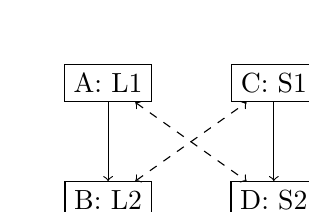
\begin{tikzpicture}
    \node[draw] (L1) {A: L1};
    \node[draw, below = of L1] (L2) {B: L2};
    \node[draw, right = of L1] (S1) {C: S1};
    \node[draw, below = of S1] (S2) {D: S2};
    \draw[->] (L1) -- (L2);
    \draw[->] (S1) -- (S2);
    \draw[<->, dashed] (L1) -- (S2);
    \draw[<->, dashed] (L2) -- (S1);
  \end{tikzpicture}
  \caption{An example aliasing and control flow graph.}
  \label{fig:cross_product:example_aliasing}
  \vspace{-10pt}
\end{wrapfigure}

To understand why, consider
Figure~\ref{fig:cross_product:example_aliasing}.  This is supposed to
indicate that both {\StateMachines} have two memory accessing
operations, that the first operation of the first {\StateMachine}
aliases with the second operation of the second {\StateMachine}, and
that the second operation of the first {\StateMachine} aliases with
the first operation of the second {\StateMachine}.  The cross-product
building algorithm will start in configuration (L1, S1), indicating
that both input {\StateMachines} are in their initial state.  These
two accesses do not alias, but must still be considered to have
cross-{\StateMachine} effects.  Otherwise, the cross-product building
algorithm will only consider one possible (arbitrarily chosen)
ordering of the two accesses, which would clearly be inadequate here.
For instance, if it chose to issue L1 before S1 it would produce the
cross-product {\StateMachine} shown in
Figure~\ref{fig:incorrect_cross_product}\footnote{Assume for the
  purposes of the example that both {\StateMachines} have already
  issued some memory accesses, so that the part of the algorithm which
  avoids considering paths where one {\StateMachine} completes
  atomically are not relevant.}, which does not model the valid memory
access sequence S1, L1, L2, S2 (or any sequence which can be obtained
from that one by exchanging non-interfering operations).  This is
clearly incorrect.  Conversely, if it had chosen to issue S1 before L1
then it would have omitted L1, S1, L2, S2.

\begin{figure}
  \begin{tikzpicture}
    \node[stateSideEffect, initial above] (AC) {\shortstack{(A, C)\\L1}};
    \node[stateSideEffect, right = of AC] (BC) {\shortstack{(B, C)\\\stIf{\happensBefore{B}{C}}}};

    \node[stateSideEffect, above right = of BC] (B) {\shortstack{B\\L2}};
    \node[stateSideEffect, right = of B] (0C) {\shortstack{($\varnothing$, C)\\S1}};
    \node[stateSideEffect, right = of 0C] (0D) {\shortstack{($\varnothing$, D)\\S2}};
    \node[stateSideEffect, right = of 0D] (001) {\shortstack{$\varnothing$\\$\happensBefore{L1}{S2}$\\$\happensBefore{L2}{S1}$}};

    \node[stateSideEffect, below right = of BC] (C) {\shortstack{B\\S1}};
    \node[stateSideEffect, right = of C] (BD) {\shortstack{(B, D)\\L2}};
    \node[stateSideEffect, right = of BD] (0D2) {\shortstack{($\varnothing$, D)\\S2}};
    \node[stateSideEffect, right = of 0D2] (002) {\shortstack{$\varnothing$\\$\happensBefore{L1}{S2}$\\$\happensBefore{S1}{L2}$}};

    \draw[->] (AC) -- (BC);
    \draw[->,ifTrue] (BC) -- (B);
    \draw[->] (B) -- (0C);
    \draw[->] (0C) -- (0D);
    \draw[->] (0D) -- (001);

    \draw[->,ifFalse] (BC) -- (C);
    \draw[->] (C) -- (BD);
    \draw[->] (BD) -- (0D2);
    \draw[->] (0D2) -- (002);
  \end{tikzpicture}
  \caption{An incorrect cross-product of the {\StateMachines} in
    Figure~\ref{fig:cross_product:example_aliasing}.  \todo{Not
      particularly clear what this actually means.}}
  \label{fig:incorrect_cross_product}
\end{figure}

Fortunately, this problem is easy to fix: the cross-product algorithm
must look ahead through the {\StateMachines} to find possible future
aliasing accesses before concluding that the current accesses are
thread-local.  In the example, from configuration (L1, S1), it could
look ahead through the second {\StateMachine} to find that L1 aliases
with S2, and is therefore not thread-local, or it could look ahead
through the first {\StateMachine} to find that S1 aliases with L2.  In
either case, it will have to generate a happens-before test for L1 and
S1, producing the cross-product {\StateMachine} shown in
Figure~\ref{fig:correct_cross_product}.  This {\StateMachine}
correctly captures all interesting interleavings of accesses of the
memory accesses.

\begin{figure}
  \begin{centering}
    \hfill
  \begin{tikzpicture}
    \node[stateSideEffect, initial] (AC) {\shortstack{(A, C)\\\stIf{\happensBefore{A}{C}}}};
    \node[stateSideEffect, below left = of AC] (A1) {\shortstack{A\\L1}};
    \node[stateSideEffect, below = of A1] (BC) {\shortstack{(B, C)\\\stIf{\happensBefore{B}{C}} }};
    \node[stateSideEffect, below left = of BC] (B) {\shortstack{B\\L2}};
    \node[stateSideEffect, below = of B] (0C) {\shortstack{($\varnothing$, C)\\S1}};
    \node[stateSideEffect, below = of 0C] (0D) {\shortstack{($\varnothing$, D)\\S2}};
    \node[stateSideEffect, below = of BC] (C1) {\shortstack{C\\S1}};
    \node[stateSideEffect, below right = of C1] (BD) {\shortstack{(B, D)\\L2}};
    \node[stateSideEffect, below = of BD] (0D2) {\shortstack{($\varnothing$, D)\\S2}};

    \node[stateSideEffect, below right = of AC] (C0) {\shortstack{C\\S1}};
    \node[stateSideEffect, below = of C0] (AD) {\shortstack{(A, D)\\\stIf{\happensBefore{A}{D}}}};
    \node[stateSideEffect, below = of AD] (A2) {\shortstack{A\\L1}};
    \node[stateSideEffect, below right = of AD] (D) {\shortstack{D\\S2}};
    \node[stateSideEffect, below = of D] (A0) {\shortstack{(A, $\varnothing$)\\L1}};
    \node[stateSideEffect, below = of A0] (B0) {\shortstack{(B, $\varnothing$)\\L2}};

    \draw[->, ifTrue] (AC) -- (A1);
    \draw[->, ifTrue] (BC) -- (B);
    \draw[->, ifTrue] (AD) -- (A2);
    \draw[->, ifFalse] (AC) -- (C0);
    \draw[->, ifFalse] (BC) -- (C1);
    \draw[->, ifFalse] (AD) -- (D);

    \draw[->] (A1) -- (BC);
    \draw[->] (C1) -- (BD);
    \draw[->] (BD) -- (0D2);
    \draw[->] (C0) -- (AD);
    \draw[->] (A2) -- (BD);
    \draw[->] (D) -- (A0);
    \draw[->] (A0) -- (B0);

    \draw[->] (B) -- (0C);
    \draw[->] (0C) -- (0D);

  \end{tikzpicture}
    \hfill
  \end{centering}
  \caption{Correct cross-product of the {\StateMachines} shown in
    Figure~\ref{fig:cross_product:example_aliasing}.  Note that the
    first state must test whether A happens before C, even though A
    and C can never alias.}
  \label{fig:correct_cross_product}
\end{figure}

\subsubsection{Other important features of the algorithm}

The cross-product building algorithm used in {\implementation} has a
number of other features not illustrated in the example:

\begin{itemize}
\item
  Atomic blocks are correctly maintained.  The output {\StateMachine}
  configurations have a further field not discussed above which
  indicates which, if either, of the two input {\StateMachines} are
  currently executing within atomic blocks.  When one {\StateMachine}
  is in an atomic block then only that {\StateMachine} is allowed to
  issue operations in the output {\StateMachine}, regardless of what
  the rules illustrated above would suggest.  Implementing
  {\stStartAtomic} and {\stEndAtomic} side-effects is then a
  simple matter of updating this field.

\item The output {\StateMachine} is not necessarily tree-structure,
  but forms a DAG of states.  For instance, in
  Figure~\ref{fig:correct_cross_product}, the (B, D) configuration is
  referenced from two memory orderings.  This means that the number of
  states in the output {\StateMachine} grows as roughly $O(nm)$, where
  $n$ is the number of states in the crashing thread {\StateMachine}
  and $m$ the number in the interfering thread one, rather than in
  proportion to the number of potential interleavings, which is
  $O(2^{\mathrm{min}(n,m)})$.  This makes it much easier to scale
  {\technique} to larger {\StateMachines}.

\item The output {\StateMachine} includes a large number of
  {\stUnreached} states.  The {\StateMachine} simplification passes
  are quite effective at removing these, but for efficiency reasons we
  would prefer to not generate them at all.  {\Implementation}
  includes a few simple rules to eliminate some of the more egregious
  ones.  For instance, in the example, no state after C in the
  crashing thread {\StateMachine} can issue any memory accesses, and
  so if the crashing thread ever reaches C before the interfering
  thread has issued any accesses then the crashing thread will
  definitely complete as-if atomically and be replaced by an
  {\stUnreached} state, and so state C in the output
        {\StateMachine} will itself be replaced by an
        {\stUnreached} state.  There is therefore no need to
        actually generate any of (\{D, true\}, \{E, false\}), (\{H,
        true\}, \{E, false\}), or (\{G, true\}, \{E, false\}).  These
        rules are generally quite obvious and unenlightening and so
        are not discussed in detail here.
\end{itemize}

\subsection{Path explosion}

One common problem in symbolic execution systems is path explosion:
the number of paths through a program rises exponentially in the size
of the program, and this can prevent na\"ive symbolic execution
systems from being applied to realistically large programs.  In the
case of \technique, there are two main causes of path explosion:

\begin{itemize}
\item
  Aliasing.  If the various simplification passes and the dynamic
  analysis cannot determine how memory accessing instructions alias
  then the symbolic execution engine must consider every possible
  aliasing pattern, of which there are $O(n^m)$, where $n$ is number
  of \state{Load} operations and $m$ the number of \state{Store} ones.
  This grows rather quickly in the number of unsolvable aliasing
  problems, especially when the number of \state{Store}s in the
  {\StateMachine} rises.  The use of lazy alias resolution helps
  mitigate this to some extent, but does not eliminate it completely.
  This represents one of the major limitations to \technique's
  scalability.
\item
  Thread interleaving.  The cross-product {\StateMachine} will have
  $O(nm)$ states, where $n$ is number of states in the read-side
  {\StateMachine} and $m$ the number in the write-side one.  The
  number of paths through the combined {\StateMachine} then grows as
  $O(2^{(nm)})$, which again grows rather quickly.
\end{itemize}

The result is that, in the common case where the read-side
{\StateMachine} consists mostly of \state{Load} operations and
write-side one mostly of \state{Store} ones, the symbolic execution
engine might have to consider up to $O((2n)^m)$ distinct paths when
evaluating the cross-product {\StateMachine}.  This is obviously
completely infeasible for even moderate values of $n$ and $m$.  For
good performance, {\technique} relies on the various simplification
and analysis techniques to reduce $n$ and $m$ to manageably small
values.  Fortunately, as discussed in the evaluation, they are able to
do so in a useful set of cases.

\section{Reproducing bugs}
\label{sect:reproducing_bugs}

\todo{I'm kind of tempted to pull this out into its own chapter.}

Given a pair of {\StateMachines} and a verification condition it is
possible to build a ``crash enforcer'': a patch to the program which
will insert delays into the program's execution in a way which will
make the bug more likely to reproduce.  This can then be used to
determine which of the many bugs reported by the prior analysis are
actually reproducible, and hence to appropriately target efforts in
fixing them.
\begin{figure}
  \begin{tabular}{ll}
    \multicolumn{2}{l}{\texttt{int *global\_ptr[];}}\\
    \hspace{-5mm}\subfigure[][Crashing thread source]{
      \texttt{
        \begin{tabular}{lll}
          \multicolumn{3}{l}{void crashing(int idx1) \{}\\
          &\multicolumn{2}{l}{if (global\_ptr[idx1])}\\
          &&*global\_ptr[idx1] = 7;\\
          \}\\
        \end{tabular}
      }
    } & \hspace{-5mm}%
    \subfigure[][Interfering thread source]{
      \texttt{
        \begin{tabular}{ll}
          \multicolumn{2}{l}{void interfering(int idx2) \{}\\
          &global\_ptr[idx2] = NULL;\\
          \}\\
          \\
        \end{tabular}
      }
    }\\
    \hspace{-5mm}\subfigure[][Crashing thread machine code]{
      \texttt{
        \begin{tabular}{rlll}
          & \multicolumn{3}{l}{crashing:} \\
          l1: & ADD & global\_ptr+idx1 & \!\!\!$\rightarrow$ reg1 \\
          l2: & LOAD & *reg1 & \!\!\!$\rightarrow$ reg2 \\
          l3: & CMP & 0, reg2 \\
          l4: & JE & l7 \\
          l5: & LOAD & *reg1 & \!\!\!$\rightarrow$ reg3 \\
          l6: & STORE & 7 & \!\!\!$\rightarrow$ *reg3 \\
          l7:
        \end{tabular}
      }
    } & \hspace{-5mm}%
    \subfigure[][Interfering thread machine code]{
      \texttt{
        \begin{tabular}{rlll}
          & \multicolumn{3}{l}{interfering:} \\
          l8: & ADD & global\_ptr+idx2 & \!\!\!$\rightarrow$ reg4 \\
          l9: & STORE & 0 & \!\!\!$\rightarrow$ *reg4 \\
          \\
          \\
          \\
          \\
          \\
        \end{tabular}
      }
    }\\
  \end{tabular}
  \caption{Example threads.}
  \label{fig:enforce:example_threads}
\end{figure}
  
Consider, for example, the threads shown in
Figure~\ref{fig:enforce:example_threads}\footnote{This example is
  discussed further in Section~\ref{sect:eval:indexed_toctou}, where
  it is referred to as the indexed\_toctou bug.}.  There is a risk
here that the crashing thread might crash if \verb|l9| is interleaved
between \verb|l2| and \verb|l5| and \verb|idx1 == idx2|.  The previous
analysis phase will detect this bug and produce the verification
condition $idx1 = idx2 \wedge \happensBefore{l2}{l9} \wedge
\happensBefore{l9}{l5}$.  This can then be used to augment the control
flow graph of the program with happens-before edges, as shown in
Figure~\ref{fig:using:example_hb_graph}.

\begin{figure}
  \centerline{
  \begin{tikzpicture}
    \node[CfgInstr] (l1) {l1: ADD global\_ptr + idx1 $\rightarrow$ reg1};
    \node[CfgInstr, below=of l1] (l2) {l2: LOAD ${\ast}reg1 \rightarrow reg2$};
    \node[CfgInstr, below=of l2] (l3) {l3: CMP $0, reg2$};
    \node[CfgInstr, below=of l3] (l4) {l4: JMP\_IF\_EQ };
    \node[CfgInstr, below=of l4] (l5) {l5: LOAD ${\ast}reg1 \rightarrow reg3$ };
    \node[CfgInstr, below=of l5] (l6) {l6: STORE $7 \rightarrow {\ast}reg3$ };
    \node[CfgInstr, below=of l6] (l7) {};
    \node[CfgInstr, right=of l1] (l8) {l8: ADD $global\_ptr + idx2 \rightarrow reg4$};
    \node[CfgInstr, below=30mm of l8] (l9) {l9: STORE $0 \rightarrow {\ast}reg4$};
    \draw[->] (l1) -- (l2);
    \draw[->] (l2) -- (l3);
    \draw[->] (l3) -- (l4);
    \draw[->,ifFalse] (l4) -- (l5);
    \draw[->,ifTrue] (l4.west) to [bend right=70] (l7);
    \draw[->] (l5) -- (l6);
    \draw[->] (l6) -- (l7);
    \draw[->] (l8) -- (l9);
    \draw[->,happensBeforeEdge] (l2) -- (l9);
    \draw[->,happensBeforeEdge] (l9) -- (l5);
  \end{tikzpicture}
  }
  \caption{CFG with happens-before edges for the example.}
  \label{fig:using:example_hb_graph}
\end{figure}

{\Technique} can make this condition more likely to be satisfied by
inserting small delays into the program's execution.  In this case,
all that needs to happen is for some thread to execute \texttt{l9}
while another thread is between \texttt{l2} and \texttt{l5}, and so
inserting a delay anywhere between \texttt{l2} and \texttt{l5} would
be sufficient.  The longer the delay, the more likely it becomes that
some other thread will execute \texttt{l9} during it, and hence the
more easily the bug will reproduce.  The performance impact of this
strategy would be roughly proportional to the frequency at which
\texttt{l2} runs, and so it would be appropriate if \texttt{l9} runs
more often than \texttt{l2}.  Alternatively, the program could be
modified such that \texttt{l9} waits for some other thread to execute
\texttt{l2}, so that \texttt{l9} can be issued as soon as \texttt{l2}
completes, which would again make it easier to reproduce the bug; in
this case, the cost would be roughly proportional to the frequency of
\texttt{l9}, making this strategy appropriate when \texttt{l2} is more
common than \texttt{l9}.

Of course, for this bug, simply reproducing the happens-before graph
is not guaranteed to reproduce the bug, because the two threads will
only interact at all when $\mathit{idx1} = \mathit{idx2}$.  An ideal
enforcer would only impose delays when there is some possibility of
this side-condition being satisfied, so as to minimise the overheads
of the enforcer when the bug is not reproduced.  This is not just a
performance requirement: inserting delays often means that the buggy
code will run less often, and so inserting delays when the bug has no
chance of reproducing will often cause the bug to reproduce
\emph{less} frequently; precisely the opposite of the desired effect.
One important complication here is that the side-condition will often
involve thread-local state from multiple threads (in this case,
$\mathit{idx1}$ is local to the crashing thread and $\mathit{idx2}$ to
the interfering one), so that no single thread can evaluate the
condition by itself.  

\begin{figure}
  \begin{centering}
    \hfill
  \begin{tikzpicture}
    \node[draw] (A) {A};
    \node[draw, above right = of A] (X) {X};
    \node[draw, below right = of X] (B) {B};
    \node[draw, above right = of B] (Y) {Y};
    \node[draw, below right = of Y] (C) {C};
    \draw[->] (A) -- (B);
    \draw[->] (B) -- (C);
    \draw[->] (X) -- (Y);
    \draw[->,happensBeforeEdge] (A) -- (X);
    \draw[->,happensBeforeEdge] (X) -- (B);
    \draw[->,happensBeforeEdge] (B) -- (Y);
    \draw[->,happensBeforeEdge] (Y) -- (C);
  \end{tikzpicture}
  \hfill
  \end{centering}
  \caption{A happens-before graph which cannot be reproduced by
    inserting a simple delay.  The bug of interest reproduces only for
    the access ordering A, X, B, Y, C.}
  \label{fig:enforce_crash:complex_hb}
\end{figure}

Figure~\ref{fig:enforce_crash:complex_hb} shows a more complex
example.  The graph would be difficult to enforce by simply inserting
fixed delays between instructions within a given thread.  Consider,
for instance, the delay between X and Y.  This must be sized so as to
increase the probability of Y happening after B, but without overly
increasing the probability of Y happening after C.  Similarly, the
delay between A and B must be sized such that B occurs after X but
before Y.  Solving that kind of constraint requires detailed
information about the program's timing, and this information is both
difficult to collect and highly configuration-specific\editorial{Cite,
  maybe?}.

{\Technique} solves these problems by modelling the program as a
message-passing system.  The core idea is to model a happens-before
ordering X before Y as a message which is sent by X, after it
completes, and collected by Y, before it starts.  In the first
example, there will be two messages, one from \texttt{l2} to
\texttt{l9} and one from \texttt{l9} to \texttt{l5}.  The desired
happens-before graph will be achieved precisely when all of these
message operations succeed.

\begin{wrapfigure}{r}{6cm}
  \vspace{-10pt}
  \hspace{-5pt}
  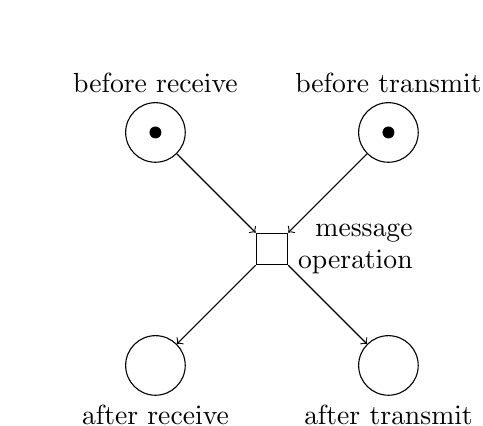
\begin{tikzpicture}
    \node[place,tokens=1,label=above:{before receive}] (beforeRx) {};
    \node[transition,below right=of beforeRx, label=right:{\shortstack[r]{message\\operation}}] (trans) {};
    \node[place,tokens=1,above right = of trans, label=above:{before transmit}] (beforeTx) {};
    \node[place,tokens=0,below left = of trans, label=below:{after receive}] (afterRx) {};
    \node[place,tokens=0,below right = of trans, label=below:{after transmit}] (afterTx) {};
    \draw[->] (beforeRx) -- (trans);
    \draw[->] (beforeTx) -- (trans);
    \draw[->] (trans) -- (afterRx);
    \draw[->] (trans) -- (afterTx);
  \end{tikzpicture}
  \caption{Petri net for the message operation.}
  \label{fig:message_petri_net}
  \vspace{-10pt}
\end{wrapfigure}
These messages are synchronous, in the sense that a message operation
cannot complete unless both the sender and the receiver are
simultaneously at the relevant instructions.  This provides a
convenient place in which to evaluate side-conditions.
Figure~\ref{fig:message_petri_net} gives a Petri net semantics for the
message operation.  One way of reading this diagram is to say that the
process starts with two threads, in the two before locations, which
are then merged into a single thread in the message operation
transition, and which then split apart into separate threads in the
two after places.  This suggests an obvious strategy for evaluating
the side-condition: if the message operation transition represents the
merging of the two threads, then it should be able to access both
threads' local state, and so should be able to evaluate the
$\mathit{idx1} = \mathit{idx2}$ side-condition.  This is the strategy
adopted by {\implementation}\footnote{There is an alternative design
  for the message passing-operation in which the message operations
  are asynchronous, so the threads never merge, but carry some of the
  sending thread's local state as a kind of payload, so that the
  side-condition can be evaluated in the receiving thread before it
  receives the message.  That would potentially allow greater
  parallelism, and hence might reduce the overhead of the enforcers,
  but at the expense of greater implementation complexity.  I have not
  investigated this alternative strategy in detail.}.

\subsection{Outline of algorithm}

At a high level, the algorithm used has the following phases:

\begin{itemize}
\item
  Examine the verification condition and extract the happens-before
  graphs which are to be reproduced.  This is discussed in
  Section~\ref{sect:enforce:slice_hb_graph}.
\item
  Decide how to evaluate the parts of the non-happens-before parts of
  the verification condition.  This is discussed in
  Section~\ref{sect:enforce:place_vcs}.
\item
  If appropriate, multiple enforcers can be combined at this point,
  which can sometimes make it easier to discover bugs if the initial
  analyses have produced a very large pool of
  candidates\editorial{This is completely trivial, so I haven't
    described how to do it, but it probably wants something
    somewhere.}.
\item
  Decide on a strategy for gaining control of the program at
  appropriate points.  Section~\ref{sect:enforce:gain_control}
  discusses how this is done.

\item
  The results of the previous phases are then combined with the plan
  interpreter, discussed in Section~\ref{sect:enforce:interpreting},
  to produce an ELF shared object which can be loaded into the target
  program to enforce the plan.
\end{itemize}

\subsection{Slicing the verification condition by happens-before graph}
\label{sect:enforce:slice_hb_graph}

\todo{This is a really complicated way of describing BDD reordering.}

{\STateMachines} and \glspl{verificationcondition} are capable of
representing data and control flow dependent happens-before graphs,
but the message passing mechanism used by \glspl{bugenforcer} is not
capable of enforcing such things.  It is now therefore necessary to
remove these dependencies.  The approach taken by {\implementation} is
to just re-express the verification condition as a function of the
happens-before graph, deriving a new verification condition for each
possible graph.  These new conditions can then be treated completely
independently.

This re-expression is itself straightforward: enumerate all of the
$\happensBeforeEdge$ expressions in the verification condition and
then consider all combinations of those expressions in turn,
generating a new verification condition for each.  This could
potentially generate $2^n$ new verification conditions, and hence
might appear to be computationally unpleasant.  In practice, it is
usually tolerable, for two main reasons:

\begin{itemize}
\item
  Most bugs do not involve a particularly large number of
  happens-before edges, and so $n$ is usually small (Musuvathi et
  al\cite{Musuvathi2007}, for instance, obtained good results while
  limiting the number of happens-before edges to at most 2).
\item
  Most bugs do not have a data-dependent happens-before pattern, and
  so usually all but one of the potentially verification conditions
  can be eliminated very quickly.  Those which do have data-dependent
  happens-before requirements will usually only have a very small
  number of interesting graphs (although it is possible to design
  artificial bugs which require an arbitrarily large number).
\end{itemize}

Even better, most of the time, behaviours which require a large number
of happens-before edges will be quite restricted in when they
reproduce, and so avoiding one easy case is negatively correlated with
avoiding the other\editorial{Huh?}.

\todo{Somewhat surprisingly, this is quite a long way from being the
  most expensive part of the analysis.  Should really try to get some
  numbers on what the expensive part actually is.}

Treating the different graphs as completely independent does not,
therefore, lead to an excessive increase in the cost of generating the
enforcer.  It does, however, lead to some inefficiency in the enforcer
itself, as it is not possible to shared common expressions between the
different bugs.  When combining completely unrelated enforcers this is
not usually a problem, as there are unlikely to be many common
expressions anyway, but this is not true when combining closely
related enforcers.  A more elegant approach would be to allow
enforcers to share a common prefix and then only have them diverge
once they encounter the data-dependent happens-before components.  I
have not implemented such an optimisation.

\subsection{Placing the evaluation of verification conditions}
\label{sect:enforce:place_vcs}

The verification condition has now been factored into a happens-before
graph and a side-condition, such that if the happens-before graph is
enforced while the side-condition holds then the bug is highly likely
to reproduce.  The next step is to decide how to evaluate the
side-condition.  This amounts to factoring the side-condition $p$ into
a set of sub-conditions $p_0, p_1, {\ldots}, p_n$ such that $p =
\wedge_i p_i$ and then attaching the $p_i$ to either nodes in the
control-flow graph or edges in the happens-before
graph\editorial{Should probably have said explicitly that the various
  inputs to the side-condition become available at different points in
  the CFG.}.  The $p_i$ are chosen such that each depends on a
different subset of the program's state, and they are placed as early
as possible in the two graphs such that all of the necessary state is
available.  The intent is to ensure that if a side-condition is
ultimately going to fail, that is detected as soon as possible, so
that the enforcer avoids imposing unnecessary delays and avoids
running the program in the interpreter for longer than is strictly
necessary.

\begin{figure}
  \begin{tikzpicture}
    \node (t1) {Thread 1};
    \node[right = 4.5cm of t1] (t2) {Thread 2};
    \node[below = of t1] (A) {$A$};
    \node[below = of A] (B) {$B$};
    \node[below = of B] (C) {$C$};
    \node[below = of C] (D) {$D_0$};
    \node[left = 4cm of D] (D1) {$D_1$};
    \node at (t2 |- A) (X) {$X$};
    \node at (t2 |- B) (Y) {$Y$};
    \node at (t2 |- D) (Z) {$Z$};
    \draw[->] (A) -- (B);
    \draw[->] (B) -- (C);
    \draw[->] (C) -- (D);
    \draw[->] (C) -- (D1);
    \draw[->] (X) -- (Y);
    \draw[->] (Y) -- (Z);
    \draw[->] (D1) to [bend right=55] (D);
    \draw[->,happensBeforeEdge] (B) to node [above] {M} (Y);
    \draw[->,happensBeforeEdge] (Z) to node [above] {N} (D);
  \end{tikzpicture}
  \center{Side condition: $\textsc{rax}_1 = 93 \wedge (\textsc{rbx}_2 =
    72 \vee \controlEdge{1}{C}{D_0}) \wedge \textsc{rcx}_1 = \textsc{rcx}_2$}
  \caption{Example control-flow and happens-before graphs.}
  \label{fig:place_conditions_example}
\end{figure}

Consider the example shown in
Figure~\ref{fig:place_conditions_example}.  Solid lines indicate
control flow within a thread and dashed lines indicate the
happens-before edges between threads which are to be enforced.  The
$D_0$ and $D_1$ \gls{cfg} nodes in the first thread represent duplicates of
the same program instruction created by the loop unrolling algorithm
(see Section~\ref{sect:derive:handling_loops}).  These \gls{cfg} nodes are
indistinguishable in the original program, but only $D_0$ can receive
the happens-before edge N.

\begin{figure}
  \begin{tikzpicture}
    \node (t1) {Thread 1};
    \node[right = 4.5cm of t1] (t2) {Thread 2};
    \node[below = of t1] (A) {$A$};
    \node[left = 0 of A] {$\textsc{rax}_1$, $\textsc{rcx}_1$};
    \node[below = of A] (B) {$B$};
    \node[left = 0 of B] {$\textsc{rax}_1$, $\textsc{rcx}_1$};
    \node[below = of B] (C) {$C$};
    \path (node cs:name=C,anchor=north east) node [below right] {\shortstack[r]{$\textsc{rax}_1$, $\textsc{rcx}_1$\\$\textsc{rbx}_2$, $\textsc{rcx}_2$}};
    \node[below = of C] (D) {$D_0$};
    \path (node cs:name=D,anchor=north west) node [below left] {\shortstack[c]{$\controlEdge{1}{C}{D_0}$,\\$\textsc{rax}_1$, $\textsc{rcx}_1$\\$\textsc{rbx}_2$, $\textsc{rcx}_2$}\!\!\!};
    \node[left = 4cm of D] (D1) {$D_1$};
    \node at (t2 |- A) (X) {X};
    \node[below right = 0 of X.north east] {$\textsc{rbx}_2$, $\textsc{rcx}_2$};
    \node at (t2 |- B) (Y) {Y};
    \node[below right = 0 of Y.north east] {\shortstack[l]{$\textsc{rax}_1$, $\textsc{rcx}_1$\\$\textsc{rbx}_2$, $\textsc{rcx}_2$}};
    \node at (t2 |- D) (Z) {Z};
    \node[below right = 0 of Z.north east] {\shortstack[l]{$\textsc{rax}_1$, $\textsc{rcx}_1$\\$\textsc{rbx}_2$, $\textsc{rcx}_2$}};
    \draw[->] (A) -- (B);
    \draw[->] (B) -- (C);
    \draw[->] (C) -- (D);
    \draw[->] (C) -- (D1);
    \draw[->] (X) -- (Y);
    \draw[->] (Y) -- (Z);
    \draw[->] (D1) to [bend right=55] (D);
    \draw[->,happensBeforeEdge] (B) to node [above] {M} node [below] {\shortstack[c]{$\textsc{rax}_1$, $\textsc{rcx}_1$\\$\textsc{rbx}_2$, $\textsc{rcx}_2$}} (Y);
    \draw[->,happensBeforeEdge] (Z) to node [above] {N} node [below] {\shortstack[c]{$\textsc{rax}_1$, $\textsc{rcx}_1$\\$\textsc{rbx}_2$, $\textsc{rcx}_2$,\\$\controlEdge{1}{C}{D_0}$}} (D);
  \end{tikzpicture}
  \caption{Figure~\ref{fig:place_conditions_example} extended to show
    input availability.}
  \label{fig:place_conditions_example:availability}
\end{figure}

The side-condition to this bug depends on various values which have to
be collected from the running program, referred to as the condition's
inputs: $\textsc{rax}_1$, $\textsc{rbx}_1$, $\textsc{rcx}_1$,
$\textsc{rcx}_2$, and $\controlEdge{1}{C}{D_0}$.  It is important not
to evaluate any part of the side condition before that part's inputs
become available.  The availability of inputs for this example is
shown in Figure~\ref{fig:place_conditions_example:availability}.

\begin{itemize}
\item $\textsc{rax}_1$ and $\textsc{rcx}_1$ represent the initial
  values of registers \textsc{rax} and \textsc{rcx} in thread 1, and
  are therefore trivially available at the start of thread 1.  The
  enforcer can copy them to its local state, when necessary, and so
  they are also available at every subsequent instruction in thread 1.
  Similarly, $\textsc{rbx}_2$ and $\textsc{rcx}_2$ are available
  throughout thread 2.
\item All of the program registers are available when evaluating the
  message edge M.  In general, the expressions available on a message
  edge will be the union of the expressions available at the sender and
  receiver of the message.
\item All of the program registers are available at instruction Y.
  This instruction receives the message M before it starts, and so
  anything which is available to M will also be available to Y.  On
  the other hand, in thread 1 the expressions available to M do not
  become available until instruction C, the instruction after the one
  which sent the message.  This asymmetry is because messages are
  received at the start of an instruction and sent at the end.
\item Likewise, the control flow expression $\controlEdge{1}{C}{D_0}$
  is available at $D_0$ and N, as these happen after instruction C
  completes and control flow expressions become available near the end
  of the instruction cycle.
\end{itemize}

The precise details of the instruction cycle, and hence precise rules
for calculating when input expressions become available, are given in
Section~\ref{sect:enforce:llis}\editorial{Well, they're kind of
  implied rather than given, but they're pretty damn obvious.
  Wouldn't hurt to be a bit more explicit, I suppose.}.

Once the input expression availability map has been calculated, the
next step is to decide how to evaluate the side condition, and in
particular at which \gls{cfg} nodes it should be evaluated.  It would,
in principle, to evaluate the entire side condition only once all of
its inputs become available, but this would be quite inefficient.  In
the example, the side condition can only be satisfied if
$\textsc{rax}_1 = 93$, and $\textsc{rax}_1$ is available before the
first message operation, so it would be undesirable to insert the
delays related to the message M when $\textsc{rax}_1 \not= 93$.  In
general, we would like to evaluate as much of the side-condition as
possible early in the \gls{cfg}, so as to exit the enforcer as soon as
possible when the condition is definitely going to fail, as this will
minimise the performance overhead.

\begin{figure}
  \centerline{
    \begin{tikzpicture}
      \node (root) [BddNode] {$\controlEdge{1}{C}{D_0}$};
      \path (node cs:name=root) ++(-2,-1.3) node (a0) [BddNode] {$\textsc{rax}_1 = 93$};
      \node (c0) [BddNode, below = of a0] {$\textsc{rcx}_1 = \textsc{rcx}_2$};
      \path (node cs:name=c0) ++(0, -3) node (true) [BddLeaf] {\true};
      \path (node cs:name=root) ++(2,-1.3) node (a1) [BddNode] {$\textsc{rax}_1 = 93$};
      \node (c1) [BddNode, below = of a1] {$\textsc{rcx}_1 = \textsc{rcx}_2$};
      \path (node cs:name=c1) ++(0, -3) node (false) [BddLeaf] {\false};
      \path (node cs:name=root) ++(0,-4.2) node (b) {$\textsc{rbx}_2 = 72$};
      \draw[BddTrue] (root) -- (a0);
      \draw[BddFalse] (root) -- (a1);
      \draw[BddTrue] (a0) to (c0);
      \draw[BddFalse] (a0) to [bend left=20] (false.north);
      \draw[BddTrue] (a1) -- (c1);
      \draw[BddFalse] (a1.east) to [bend left=90] (false.east);
      \draw[BddTrue] (c0) -- (true);
      \draw[BddFalse] (c0.east) to [bend left=30] (false.north);
      \draw[BddTrue] (c1) -- (b);
      \draw[BddFalse] (c1) -- (false);
      \draw[BddTrue] (b) -- (true);
      \draw[BddFalse] (b) -- (false);
    \end{tikzpicture}
  }
  \caption{The side-condition in
    Figure~\ref{fig:place_conditions_example} expressed as a BDD,
    assuming the variable ordering $\controlEdge{1}{C}{D_0}$,
    $\textsc{rax}_1 = 93$, $\textsc{rcx}_1 = \textsc{rcx}_2$,
    $\textsc{rbx}_2 = 72$.}
  \label{fig:place_conditions_example:bdd1}
\end{figure}

{\Technique} represents its side-conditions internally as BDDs, such
as that shown in Figure~\ref{fig:place_conditions_example:bdd1}.  The
variable ordering within the BDD is largely arbitrary, and will not
necessarily match closely with the order in which input expressions
become available in the program \gls{cfg}.  In the example, the first
variable in the BDD is the control-flow expression, but this is one of
the last input expressions to become available, making it difficult to
evaluate any part of the BDD early.

\begin{figure}
  \centerline{
    \begin{tabular}{ccccc}
      \begin{tikzpicture}
        \node (root) [BddNode,color=blue] {$\textsc{rax}_1 = 93$};
        \node (alpha) [BddNode, below = of root] {$\controlEdge{1}{C}{D_0}$};
        \node (c0) [BddNode, below = of alpha] {$\textsc{rcx}_1 = \textsc{rcx}_2$};
        \path (node cs:name=c0,anchor=east) node (c1) [BddNode,right] {$\textsc{rcx}_1 = \textsc{rcx}_2$};
        \path (barycentric cs:c0=0.5,c1=0.5) ++(0.2,-0.8) node (b) [BddNode, below] {$\textsc{rbx}_2 = 72$};
        \path (node cs:name=c1,anchor=south) ++(0,-2) node (false) [BddLeaf] {\false};
        \node (true) at (c0 |- false) [BddLeaf] {\true};
        \draw[BddTrue] (root) -- (alpha);
        \draw[BddFalse] (root.east) to [bend left=45] (false);
        \draw[BddTrue] (alpha) -- (c0);
        \draw[BddFalse] (alpha) -- (c1);
        \draw[BddTrue] (c0) -- (true);
        \draw[BddFalse] (c0) to [bend left=30] (false);
        \draw[BddTrue] (c1) -- (b);
        \draw[BddFalse] (c1) -- (false);
        \draw[BddTrue] (b) -- (true);
        \draw[BddFalse] (b) -- (false);
      \end{tikzpicture} & \raisebox{30mm}{$=$} & \raisebox{22mm}{\begin{tikzpicture}
        \node (root) [BddNode,color=blue] {$\textsc{rax}_1 = 93$};
        \node (true) at (-0.6,-1) [BddLeaf] {\true};
        \node (false) at (0.6,-1) [BddLeaf] {\false};
        \draw[BddTrue] (root) -- (true);
        \draw[BddFalse] (root) -- (false);
      \end{tikzpicture}} & \raisebox{30mm}{$\bigwedge$} & \raisebox{16mm}{\begin{tikzpicture}
        \node (root) [BddNode] {$\controlEdge{1}{C}{D_0}$};
        \path (node cs:name=root) ++ (-1.5,-1) node (c0) [BddNode] {$\textsc{rcx}_1 = \textsc{rcx}_2$};
        \path (node cs:name=root) ++ (1.5,-1) node (c1) [BddNode] {$\textsc{rcx}_1 = \textsc{rcx}_2$};
        \node (b) at (root |- 0,-1.8) [BddNode] {$\textsc{rbx}_2 = 72$};
        \node (true) [BddLeaf, below = of c0] {\true};
        \node (false) [BddLeaf, below = of c1] {\false};
        \draw[BddTrue] (root) -- (c0);
        \draw[BddFalse] (root) -- (c1);
        \draw[BddTrue] (c0) -- (true);
        \draw[BddFalse] (c0) to [bend right=20] (false);
        \draw[BddTrue] (c1) -- (b);
        \draw[BddFalse] (c1) -- (false);
        \draw[BddTrue] (b) -- (true);
        \draw[BddFalse] (b) -- (false);
      \end{tikzpicture}} \\
      (a) Reordered BDD & \multicolumn{3}{c}{\parbox{4cm}{(b) Condition evaluatable at $A$}} & (c) Residual condition
    \end{tabular}
  }
  \caption{Factorisation of the BDD in
    Figure~\ref{fig:place_conditions_example:bdd1} at CFG node $A$.
    $\textsc{rax}_1$ and $\textsc{rcx}_1$ are the only available input
    expressions.  Evaluatable BDD variables are shown in blue.}
  \label{fig:place_conditions_example:instr_a}
\end{figure}

The problem becomes far easier if the side-condition BDD is re-ordered
to reflect the order in which the input expressions become available.
The leftmost part of Figure~\ref{fig:place_conditions_example:instr_a}
shows how this is done for \gls{cfg} node $A$.  The available inputs are
$\textsc{rax}_1$ and $\textsc{rcx}_1$, and so the only evaluatable BDD
variable is $\textsc{rax}_1 = 93$, and so this variable is moved to
the root of the BDD.  The BDD can then be factorised into a component
which is evaluatable at \gls{cfg} node $A$, (b), and a residual which must
be evaluated after $A$, (c), such that (b)~$\wedge$~(c) is equal to
the original side-condition.

The factorisation algorithm itself is reasonably simple.  To build the
evaluatable component, {\technique} replaces all of the nodes which
test unevaluatable variables with edges to \true; to build the
residual component, it removes all edges from an evaluatable variable
to \false.  The usual BDD reduction rules are then used to convert the
result back into a BDD.

The most important property of this algorithm is that it produces a
correct factorisation of the side condition.  In other words, if the
algorithm decomposes $p$ into $p_0$ and $p_1$ then $p = p_0 \wedge
p_1$.  This is easiest to see by considering the paths through the
BDD: paths which test only evaluatable variables and end at \false
will be preserved in the evaluatable component of the result, and all
of the other paths will be preserved in the unevaluatable one.  If all
of the paths through the BDD are preserved then the BDD behaviour is
as well.

\todo{Should arguably try to show that it's a good factorisation, in
  the sense of genuinely finding the strongest evaluatable
  precondition, and I think it is, but the proof is pretty damn
  awkward.  Might also be worth talking about perf: BDD reordering has
  a pretty hideous worst-case complexity, which we avoid mostly by
  means of obscure implementation details in the main analysis pass.}

\todo{Could maybe move this to related work?}  This can be thought of
as a kind of predicate abstraction problem~\needCite{}.  Cavada et
al.\cite{Cavada2007} presented an algorithm similar to this one in a
slightly different context.  The key difference is that the
{\technique} algorithm will sometimes retain evaluatable variables in
the unevaluatable component of the condition, when there are complex
relationships between the evaluatable and unevaluatable variables.
The Cavada algorithm, on the other hand, partitions the condition into
a component which is completely evaluatable and one which is
completely unevaluatable.  This can sometimes force them to
approximate the condition.  If {\technique} were to do that, part of
the side-condition would remain unevaluated at the end of the
\gls{CFG} fragment, which might lead to unnecessary message operations
and hence poor performance.

\begin{figure}
  \centerline{
    \begin{tikzpicture}
      \node (b) [BddNode, color=blue] {$\textsc{rbx}_2 = 72$};
      \node (a) [BddNode, below = 2 of b] {$\textsc{rax}_1 = 93$};
      \node (c) [BddNode, below = of a] {$\textsc{rcx}_1 = \textsc{rcx}_2$};
      \node (true) [BddLeaf, below = of c] {\true};
      \node (false) [BddLeaf, right = of true] {\false};
      \node (alpha) at (false |- 1,-1.3) [BddNode] {$\controlEdge{1}{C}{D_0}$};
      \draw[BddTrue] (b) -- (a);
      \draw[BddFalse] (b) -- (alpha);
      \draw[BddTrue] (alpha) -- (a);
      \draw[BddFalse] (alpha) -- (false);
      \draw[BddTrue] (a) -- (c);
      \draw[BddFalse] (a) to [bend left=20] (false);
      \draw[BddTrue] (c) -- (true);
      \draw[BddFalse] (c) -- (false);
    \end{tikzpicture}
  }
  \caption{Reordering of the BDD in
    Figure~\ref{fig:place_conditions_example:bdd1} at CFG node $X$.
    $\textsc{rbx}_2$ and $\textsc{rcx}_2$ are the only available input
    expressions.  Evaluatable BDD variables are shown in blue. In this
    case, no non-trivial factorisation is possible.}
\end{figure}

The residual BDD which is unevaluatable at $A$ must now be propagated
through the graph until we find some place at which it can be
evaluated.  The first place we encounter, $B$, has the same available
input expression set as $A$, and so no further side-conditions can be
evaluated here.  The M edge, however, does have more available input
expressions, and so can make some progress.  The factorisation is
shown in Figure~\ref{fig:place_conditions_example:message_m}.  Note
that the residual condition here includes an evaluatable variable,
$\textsc{rbx}_2 = 72$.  In principle, this could be evaluated as part
of this message operation, but doing so would never allow the enforcer
to exit early, and so would not be helpful.

\begin{figure}
  \centerline{
    \begin{tabular}{ccccc}
      \begin{tikzpicture}
        \node (c) [BddNode,color=blue] {$\textsc{rcx}_1 = \textsc{rcx}_2$};
        \node (b) [BddNode,below = of c,color=blue] {$\textsc{rbx}_2 = 72$};
        \node (true) [BddLeaf, below = 2 of b] {\true};
        \node (false) [BddLeaf, right = of true] {\false};
        \path (node cs:name=false) ++(0,1.3) node (alpha) [BddNode] {$\controlEdge{1}{C}{D_0}$};
        \draw[BddTrue] (c) -- (b);
        \draw[BddFalse] (c) to [bend left=30] (false);
        \draw[BddTrue] (b) -- (true);
        \draw[BddFalse] (b) -- (alpha);
        \draw[BddTrue] (alpha) -- (true);
        \draw[BddFalse] (alpha) -- (false);
      \end{tikzpicture}
      & \raisebox{23mm}{$=$} &
      \raisebox{15mm}{
        \begin{tikzpicture}
          \node (c) [BddNode, color=blue] {$\textsc{rcx}_1 = \textsc{rcx}_2$};
          \path (node cs:name=root) ++(-0.6,-1) node (true) [BddLeaf] {\true};
          \path (node cs:name=root) ++(0.6,-1) node (false) [BddLeaf] {\false};
          \draw[BddTrue] (c) -- (true);
          \draw[BddFalse] (c) -- (false);
        \end{tikzpicture}
      }
      & \raisebox{23mm}{$\bigwedge$} &
      \raisebox{8mm}{
        \begin{tikzpicture}
          \node (b) [BddNode,color=blue] {$\textsc{rbx}_2 = 72$};
          \node (true) [BddLeaf, below = 2 of b] {\true};
          \node (false) [BddLeaf, right = of true] {\false};
          \path (node cs:name=false) ++(0,1.3) node (alpha) [BddNode] {$\controlEdge{1}{C}{D_0}$};
          \draw[BddTrue] (b) -- (true);
          \draw[BddFalse] (b) -- (alpha);
          \draw[BddTrue] (alpha) -- (true);
          \draw[BddFalse] (alpha) -- (false);
        \end{tikzpicture}
      }\\
      Reordered BDD & \multicolumn{3}{c}{Condition evaluatable at M} & Residual condition
    \end{tabular}
  }
  \caption{Factorisation of the BDD in
    Figure~\ref{fig:place_conditions_example:bdd1} at message edge M.}
  \label{fig:place_conditions_example:message_m}
\end{figure}

There is a slight subtlety here: how should we determine the input
condition to the factorisation algorithm when the place for which we
are performing the factorisation has multiple predecessors?  In this
case, the edge M is preceded by both $B$ and $Y$, and they have
different residual side conditions, and it is not immediately obvious
how to combine them.  The correct answer is to merge the predecessors
using $\vee$ for message edges and $\wedge$ at control flow joins.
This is because with a message edge, both incoming edges are taken, as
both threads must reach the message operation, whereas in a control
flow join only one of the incoming edges will be taken in any given
execution.  \todo{Not sure how clear that is.}

Once the algorithm has decided on the side condition for message M it
can move on to calculating the side-conditions for M's successor \gls{cfg}
nodes, $Y$ and $C$.  In this case, the set of available input
expressions does not change at either of these nodes, and so this is
trivial, and likewise for $Y$'s successor $Z$.  The message N,
however, does allow further side-conditions to be evaluated, as shown
in Figure~\ref{fig:place_conditions_example:message_n}.  All of the
input expressions are available when this message operation is
performed, and so the entire side-condition is evaluatable and the
residual condition is just \true.  The entire side-condition has now
been placed on the control flow graph.  The results are shown in
Figure~\ref{fig:place_conditions_example:result}.

\begin{figure}
  \centerline{
    \begin{tabular}{ccccc}
      \begin{tikzpicture}
        \node (b) [BddNode,color=blue] {$\textsc{rbx}_2 = 72$};
        \node (true) [BddLeaf, below = 2 of b] {\true};
        \node (false) [BddLeaf, right = of true] {\false};
        \path (node cs:name=false) ++(0,1.3) node (alpha) [BddNode, color=blue] {$\controlEdge{1}{C}{D_0}$};
        \draw[BddTrue] (b) -- (true);
        \draw[BddFalse] (b) -- (alpha);
        \draw[BddTrue] (alpha) -- (true);
        \draw[BddFalse] (alpha) -- (false);
      \end{tikzpicture}
      & \raisebox{15mm}{$=$} &
      \begin{tikzpicture}
        \node (b) [BddNode,color=blue] {$\textsc{rbx}_2 = 72$};
        \node (true) [BddLeaf, below = 2 of b] {\true};
        \node (false) [BddLeaf, right = of true] {\false};
        \path (node cs:name=false) ++(0,1.3) node (alpha) [BddNode, color=blue] {$\controlEdge{1}{C}{D_0}$};
        \draw[BddTrue] (b) -- (true);
        \draw[BddFalse] (b) -- (alpha);
        \draw[BddTrue] (alpha) -- (true);
        \draw[BddFalse] (alpha) -- (false);
      \end{tikzpicture}
      & \raisebox{15mm}{$\bigwedge$} &
      \raisebox{13mm}{
        \begin{tikzpicture}
          \node (true) [BddLeaf] {\true};
        \end{tikzpicture}
      }\\
      Reordered BDD & \multicolumn{3}{c}{Condition evaluatable at $A$} & Residual condition\\
    \end{tabular}
  }
  \caption{Factorisation of the BDD in
    Figure~\ref{fig:place_conditions_example:bdd1} at message edge N.
    Every variable is now evaluatable, and so the residual condition
    is just \true.}
  \label{fig:place_conditions_example:message_n}
\end{figure}

\begin{figure}
  \begin{tikzpicture}
    \node (t1) {Thread 1};
    \node[right = 4.5cm of t1] (t2) {Thread 2};
    \node[below = of t1] (A) {$A$};
    \node[left = 0 of A] {$\textsc{rax}_1 = 93$};
    \node[below = of A] (B) {$B$};
    \node[below = of B] (C) {$C$};
    \node[below = of C] (D) {$D_0$};
    \node[left = 4cm of D] (D1) {$D_1$};
    \node at (t2 |- A) (X) {$X$};
    \node at (t2 |- B) (Y) {$Y$};
    \node at (t2 |- D) (Z) {$Z$};
    \draw[->] (A) -- (B);
    \draw[->] (B) -- (C);
    \draw[->] (C) -- (D);
    \draw[->] (C) -- (D1);
    \draw[->] (X) -- (Y);
    \draw[->] (Y) -- (Z);
    \draw[->] (D1) to [bend right=55] (D);
    \draw[->,happensBeforeEdge] (B) to node [above] {M} node [below] {$\textsc{rcx}_1 = \textsc{rcx}_2$} (Y);
    \draw[->,happensBeforeEdge] (Z) to node [above] {N} node [below] {\shortstack{$\textsc{rbx}_2 = 72 \vee$\\$\controlEdge{1}{C}{D_0}$}} (D);
  \end{tikzpicture}
  \caption{Final placement of side-condition checks for the example
    control flow graph in Figure~\ref{fig:place_conditions_example}}
  \label{fig:place_conditions_example:result}
\end{figure}

\subsection{Enforcing the plan}
\label{sect:enforce:interpreting}

Previous sections described how to find the desired happens-before
graph, how to turn that into a message-passing system, and how to
place the components of the side-condition on the control-flow graph.
Collectively, these form the crash enforcement plan.  It remains to
show how to actually use this plan to trigger the bug.

One way to think about this problem is to treat the plan as a program
which does the same thing as the original program, but with additional
operations which make it more likely that the bug will reproduce.
Consider, for example the bug shown in
Figure~\ref{fig:enforcement:example_bug}, and its crash enforcement
plan shown in Figure~\ref{fig:enforcement:example_bug:plan}.  The plan
can be regarded as a replacement for instructions {\tt a} and {\tt c}
in the original program.  The replacement for {\tt a} will behave like
this:

\begin{itemize}
\item Check that $\mathtt{loc1} \not= 7$.  If this condition fails,
  the replacement returns to the original version of instruction {\tt
    a} and the program can then resume normal operation.
\item Emulate the program's instruction {\tt a}.  In this case, that
  means loading from {\tt loc1} and storing the result in local
  variable {\tt x}.
\item Send a message to the other thread, so as to implement the first
  happens-before edge.  Message operations are synchronous in
  {\implementation}, and so this means waiting for some other thread
  to arrive at the other side of the message passing operation.  If no
  other thread arrives within a timeout then the operation fails, so
  the whole plan fails and the thread resumes normal operation.
\item If the thread manages to send its first message, it must
  immediately wait to receive its second one.  This time, the message
  operation is the last step of the plan for this thread, and so
  regardless of whether it succeeds or fails the thread will resume
  normal operation at instruction {\tt b}.
\end{itemize}

The replacement for {\tt c} is similar:

\begin{itemize}
\item The replacement starts by receiving the first message.  This
  will, again, involve waiting for another thread to arrive, and might
  fail.
\item Assuming the message operation succeeds, the replacement will
  then move on to emulating the original program instruction {\tt c}
  by setting {\tt loc1} to 7.
\item The thread can then complete its part of the enforcement plan by
  sending the second message.  Once again, this will involve waiting
  for the other thread to reach its side of the message operation.
\item The thread can then resume normal operation at whatever
  instruction comes after {\tt c}.
\end{itemize}

\begin{figure}
  {\hfill}
  \begin{subfloat}
    \parbox{4cm}{
      \begin{tabular}{ll}
        {\tt a:} & {\tt x = loc1;}\\
        {\tt b:} & {\tt y = loc1;}\\
        & {\tt assert(x == y);}
      \end{tabular}
    }
    \caption{Crashing thread}
  \end{subfloat}
  {\hfill}
  \begin{subfloat}
    \parbox{3.2cm}{\tt c: loc1 = 7;}\\
    \caption{Interfering thread}
  \end{subfloat}
  {\hfill}
  \begin{subfloat}
    $\happensBefore{a}{c} \wedge \happensBefore{c}{b} \wedge \mathtt{loc1} \not= 7$
    \caption{Generated verification condition}
  \end{subfloat}
  {\hfill}
  \caption{An example bug}
  \label{fig:enforcement:example_bug}
\end{figure}

\begin{figure}
  \begin{tikzpicture}
    \node (n0m) {Crashing thread};
    \node (n00) [CfgInstr, below = of n0m] {\shortstack{Gain control at\\instruction {\tt a}}};
    \node (n01) [CfgInstr, below = of n00] {Require $loc1 \not= 7$};
    \node (nm1) [CfgInstr, left = of n01] {\shortstack{Return to\\instruction {\tt a}}};
    \node (n02) [CfgInstr, below = of n01] {\tt a: x = loc1};
    \node (n03) [CfgInstr, below = of n02] {Send message 1};
    \node (n04) [below = of n03] {};
    \node (n05) [below = of n04] {};
    \node (n06) [below = of n05] {};
    \node (n07) [below = of n06, CfgInstr] {Receive message 2};
    \node (n08) [below = of n07, CfgInstr] {\shortstack{Return to\\instruction {\tt b}}};
    \node (n1m) [right = of n0m] {Interfering thread};
    \node (n10) [CfgInstr, right = of n00] {\shortstack{Gain control at\\instruction {\tt b}}};
    \node (n11) [below = of n10] {};
    \node (n12) [below = of n11] {};
    \node (n13) [below = of n12] {};
    \node (n14) [below = of n13, CfgInstr] {Receive message 1};
    \node (n24) [right = of n14, CfgInstr] {\shortstack{Return to\\instruction {\tt c}}};
    \node (n15) [below = of n14, CfgInstr] {\tt c: loc1 = 7};
    \node (n16) [below = of n15, CfgInstr] {Send message 2};
    \node (n17) [below = of n16] {};
    \node (n18) [below = of n17, CfgInstr] {\shortstack{Return to instruction\\after {\tt c}}};

    \draw[->] (n00) -- (n01);
    \draw[->] (n01) -- (n02);
    \draw[->] (n02) -- (n03);
    \draw[->] (n03) -- (n07);
    \draw[->] (n07) -- (n08);
    \draw[->] (n10) -- (n14);
    \draw[->] (n14) -- (n15);
    \draw[->] (n15) -- (n16);
    \draw[->] (n16) -- (n18);

    \draw[->,ifFalse] (n01) -- (nm1);
    \draw[->,ifFalse] (n03.west) to [bend right = 45] (n08.west);
    \draw[->,ifFalse] (n07.west) to [bend right = 45] (n08.west);
    \draw[->,ifFalse] (n14) -- (n24);
    \draw[->,ifFalse] (n16.east) to [bend left = 45] (n18);

    \draw[happensBeforeEdge,->] (n03) -- (n14);
    \draw[happensBeforeEdge,->] (n16) -- (n07);
  \end{tikzpicture}
  \caption{Crash enforcement plan for the bug in
    Figure~\ref{fig:enforcement:example_bug}.  Dashed lines indicate
    message passing operations, and dotted ones indicate error paths.}
  \label{fig:enforcement:example_bug:plan}
\end{figure}

At the highest level of abstraction, this is precisely what
{\implementation}'s enforcers will do if asked to enforce that crash
enforcement plan.  There are, however, two important complications.

Most obviously, the enforcer must somehow identify the crashing and
interfering threads.  When building the plan, {\technique} assumes
that there are precisely two threads in the program, and that those
threads are easily identified.  The enforcers operate on a real
program, which might contain an arbitrary number of threads, and must
somehow select which of these concrete threads correspond to which of
the two abstract threads in the plan.  Less obviously, the
happens-before edges in the plan are expressed between nodes in the
unrolled \gls{cfg} (see Section~\ref{sect:derive:handling_loops}), and do
not necessarily correspond closely to instructions in the actual
program.  The plan might require different actions at different \gls{cfg}
nodes which are hard to distinguish in a running program.

The solution to these problems is the same: to decide as much as
possible lazily.  When {\implementation} encounters a branch in the
unrolled \gls{cfg} which does not correspond to one in the program \gls{cfg}, it
does not try to figure out which way it should go immediately, but
instead defers the decision for as long as possible by forking its
state, with one fork taking one branch of the unrolled \gls{cfg} and the
other taking the other, and maintains both forks until it becomes
clear which fork was correct.  Similarly, if it has a choice of
synchronising between several possible threads, it creates sufficient
forks of its internal state to represent synchronising with each of
them, and then decides later on which fork is correct\footnote{Note
  that these forks are entirely internal to the enforcer itself,
  rather than, for instance, being implemented with the \texttt{fork}
  system call.}.

The result is conceptually similar to the power set construction used
to simulate non-deterministic finite state automata using
deterministic ones\needCite{}.  A non-deterministic FSA can contain
branches which are ambiguous at the point where they occur, but can be
resolved by looking ahead through the automaton to discover which ones
will eventually succeed.  These semantics can be implemented in a
deterministic FSA, where every branch must be immediately unambiguous,
using the power set construction.  The idea here is for each state in
the deterministic FSA to represent a set of states in the
non-deterministic one, so that any ambiguity in the original automaton
can be resolved by moving to every possible successor state at the
same time.  If any of those successors eventually succeed then the
whole automaton succeeds.  There are, in effect, two models of
computation involved here: a low level one, which allows this kind of
non-deterministic choice, and a high level one, which does not.  The
states of the high level model are formed from sets of states of the
low level one.

{\Implementation}'s plan interpreter is structured in a similar way.
The low level interpreter implements the obvious plan semantics
discussed in the example above, using an operator similar to
non-deterministic choice when it does not have enough information to
immediately implement an operation, and the high level interpreter
then implements the choice operator by maintain sets of low level
interpreters.  Following the analogy, I start by describing what the
low level interpreter does, using non-deterministic choice operators,
and then explain how the high level interpreter implements those
operators.

\subsubsection{The low-level interpreter}
\label{sect:enforce:llis}

The low-level interpreter, or LLI, runs some simple stages in a tight
loop:

\begin{itemize}
\item \textbf{Sample} Look at the thread's registers, determine which
  ones might be needed to evaluate later side-conditions, and copy the
  appropriate registers to the LLI's local state.

\item \textbf{RX} Receive any messages required by the plan.  Message
  operations are discussed below.

\item \textbf{Emul} Emulate the instruction in the original program.
  Implementing this is moderately subtle, as it is the only phase in
  the LLI loop which has effects which are visible to the original
  program (beyond adjusting the timing).  This means that the enforcer
  must be careful to emulate instructions the right number of times,
  regardless of how many LLIs happen to be active at the time.
  {\Technique}'s design ensures that every LLI in a program thread
  will reach the \textbf{Emul} state at the same time, and will be
  executing the same program instruction\footnote{They might, however,
    be executing at different points in the unrolled \gls{cfg}, as a single
    program instruction can correspond to multiple \gls{cfg} nodes.}, and so
  this is straightforward to arrange

\item \textbf{TX} Send any messages required by the plan.

\item \textbf{Succ} Determine which node in the unrolled \gls{cfg} the
  thread is going to execute next.  In the low-level interpreter, this
  is very easy: compare the instruction pointer of the next
  instruction (generated by the \textbf{Emul} phase) to the
  instruction pointers of all of the potential successor nodes in the
  unrolled \gls{cfg} and select one using the non-deterministic choice
  operator.  If there are no possible successors then the plan has
  failed and the low-level interpreter exits.
\end{itemize}

A new low-level interpreter is started whenever any thread in the
program reaches the starting point of any of the \glspl{cfg} involved in one
of the happens-before graphs which are to be enforced\editorial{Orphan
  sentence?}.

The LLI message operation is illustrated in
Figure~\ref{fig:enforce:lli_message}.  The operation starts by
selecting a remote LLI with which to perform the message operation.
If this is the first message operation performed by this LLI then it
will select its peer using a non-deterministic choice operator,
described in Section~\ref{sect:enforce:hli_messages}, and bind to it.
Otherwise, the LLI will just select its bound LLI.  In either case,
the LLI will wait for its remote LLI to arrive.  The two LLIs are then
merged together to perform the message operation itself, by evaluating
the side condition and copying state between the two LLIs, after which
they are unmerged and continue at the appropriate place in the LLI
loop.  \todo{Binding should maybe be mentioned a little bit sooner?}

\begin{figure}
  \centerline{
  \begin{tikzpicture}
    \node (n1m) {\textbf{RX}};
    \node (n10) [below = of n1m] {$t \leftarrow$ select remote LLI};
    \node (n11) [below = of n10] {Wait for t};
    \node (n01) [left = of n11] {fail};
    \node (n22) [below right = of n11] {Merge LLIs};
    \node (n31) [above right = of n22] {Wait for $t'$};
    \node (n41) [right = of n31] {fail};
    \node (n30) [above = of n31] {$t' \leftarrow$ select remote LLI};
    \node (n3m) [above = of n30] {\textbf{TX}};
    \node (n23) [below = of n22] {Evaluate side condition};
    \node (n43) at (n23 -| n41) {fail};
    \node (n24) [below = of n23] {Copy state between LLIs};
    \node (n24b) [below = of n24] {Unmerge LLIs};
    \node (dummy) [below = of n24b] {};
    \node (n15) at (dummy -| n11) {Advance to \textbf{Emul}};
    \node (n35) at (dummy -| n31) {Advance to \textbf{Succ}};
    \draw[->] (n1m) -- (n10);
    \draw[->] (n10) -- (n11);
    \draw[->] (n11) -- (n22);
    \draw[->] (n3m) -- (n30);
    \draw[->] (n30) -- (n31);
    \draw[->] (n31) -- (n22);
    \draw[->] (n22) -- (n23);
    \draw[->] (n23) -- (n24);
    \draw[->] (n24) -- (n24b);
    \draw[->] (n24b) -- (n15);
    \draw[->] (n24b) -- (n35);
    \draw[->,ifFalse] (n11) -- (n01);
    \draw[->,ifFalse] (n31) -- (n41);
    \draw[->,ifFalse] (n23) -- (n43);
    \draw[->,style={dashed}] (n11) -- (n15);
    \draw[->,style={dashed}] (n31) -- (n35);
  \end{tikzpicture}
  }
  \caption{Message operation in the low-level interpreter.}
  \label{fig:enforce:lli_message}
\end{figure}

There are two ways for this algorithm to fail.  The simplest is that
the side-condition might evaluate to false, in which case both LLIs
fail and return the program to normal operation.  The timeouts are
more interesting.  There are several reasons why one of the wait steps
might time out:

\begin{itemize}
\item
  If this is the first message operation in the LLI, a timeout usually
  indicates that, for whatever reason, the program is not going to run
  the two desired fragments of code in parallel.  {\Technique}
  responds by having the LLI which timed out exit, allowing the
  program thread to return to normal operation.

\item
  If this is not the first message operation, a timeout usually
  indicates that the program has some existing synchronisation which
  will prevent the bug from reproducing.  The \textbf{Emul} step in
  the LLI cycle includes running any synchronisation operations which
  were present in the original program, which might cause there to be
  additional edges in the happens-before graph beyond those which
  {\technique} is aware of.  If these additional edges complete a
  cycle then attempting to enforce the bug-causing ordering will lead
  to a deadlock, which is then detected as a timeout in a message
  operation\footnote{{\Technique} has some knowledge of simple
    synchronisation operations such as \texttt{pthread\_mutex\_lock},
    and will avoid trying to enforce bugs if this knowledge is
    sufficient to show that the HB graph contains a cycle, but this is
    incomplete (in particular, it does not know about locks acquired
    before the enforcer starts), and cannot hope to cover all
    programmer-implemented synchronisation operations\cite{Xiong2010},
    and so there will always be a risk of one of these cycles
    forming.}.

  When a timeout does happen, the LLI which suffered the time out
  must, of course, exit.  Less obviously, the LLI with which it had
  previously communicated should also exit: any future message
  operations which that LLI attempts will definitely fail, and so
  there is no point continuing to run it in the enforcer.
\end{itemize}


\subsubsection{Implementing the \textbf{Succ} phase in the high-level interpreter}
\label{sect:enforce:succ}

The low-level interpreter described in Section~\ref{sect:enforce:llis}
is both correct and conceptually simple, but impossible to implement
directly due to the non-deterministic choice operators.  This section
describes how to emulate those operators in a realisable fashion.  As
discussed previously, the basic approach is to switch from emulating
the LLI itself to emulating sets of LLIs, so that the choice operators
can be implemented by adding more LLIs to these sets and an LLI exit
can be implemented by removing one.  The resulting interpreter is
referred to\editorial{by whom?} as the high-level interpreter, or HLI.

The simplest use of the operator is in the \textbf{Succ} phase.  The
aim of this phase in the LLI is to determine which node in the
unrolled \gls{cfg} a given program thread is going to execute next.  The
equivalent operation in the HLI is to convert the current set of LLIs
into a new set of LLIs, where each of the new LLIs is formed by taking
one of the old LLIs and updating its location in the unrolled \gls{cfg} in a
way which is consistent with the results of the \textbf{Emul} phase.
The new set of LLIs is given by
\begin{displaymath}
\{l' | l \in \mathit{llis}, n'.\mathrm{RIP} = \mathbf{Emul}.\mathrm{RIP}, (l.n, n') \in \mathit{CFG}, l' = l[n = n'] \}
\end{displaymath}

This perhaps deserves further explanation:

\begin{itemize}
\item $\mathit{llis}$ is the current set of LLIs, and $l$ is a member of it.
  $l'$ is a member of the new set of LLIs.
\item $n'$ is a node in the unrolled \gls{cfg}.
\item $l.n$ is LLI $l$'s current node in the unrolled \gls{cfg}.  $l[n =
  n']$ is a new LLI constructed by taking the LLI $l$ and setting its
  current \gls{cfg} node to $n'$.
\item $n'.\mathrm{RIP}$ is the raw instruction pointer associated with
  the \gls{cfg} node $n'$.  $\mathbf{Emul}.\mathrm{RIP}$ is the raw
  instruction pointer which was generated by the $\mathbf{Emul}$
  phase.
\item $(l.n, n') \in \mathit{CFG}$ is true precisely when $n'$ is one
  of the successors of $l.n$ in the unrolled \gls{cfg}.
\end{itemize}

In other words, the resulting set will contain one LLI for every
combination of existing LLI and \gls{cfg} node, provided that the new \gls{cfg}
node is a successor of the current \gls{cfg} node and provided that the new
\gls{cfg} node's raw instruction pointer matches that produced by the
\textbf{Emul} phase.  It is important to note that all of the
successors will have the same raw instruction pointer; this is
necessary to correctly implement the \textbf{Emul} phase of the next
instruction cycle.

It is perhaps informative to consider what happens to the individual
LLIs in the input set.  There are four interesting cases:

\begin{itemize}
\item The common case is that the \gls{cfg} node has precisely one successor
  node which matches the raw address of the next instruction.  The LLI
  has a single successor.  In effect, all that has happened is that
  the LLI has moved from its current node in the \gls{cfg} to one of that
  node's successors.

\item The LLI might have reached the end of the unrolled \gls{cfg}, as
  indicated by a special marker on the \gls{cfg} node, and has hence
  completed its part of the plan.  The LLI's node in the \gls{cfg} will have
  no successors, and so the LLI will not contribute anything to the
  new set of LLIs.  If another LLI has completed the other part of the
  plan then the bug should reproduce soon.

\item It might be that the \gls{cfg} is not finished, but none of this
  node's successors match up with the raw address of the next
  instruction to be executed.  In this case, the plan has failed.
  Again, this LLI has no successors, but this time the bug is unlikely
  to reproduce.  The enforcer must continue running the program in the
  hope that some other LLI will complete the plan.

\item The \gls{cfg} node might have multiple matching successors.  The LLI
  will have multiple successors, one for each possible successor,
  allowing the enforcer to determine lazily which successor was
  correct.
\end{itemize}

\subsubsection{Implementing message operations in the high-level interpreter}
\label{sect:enforce:hli_messages}

As discussed previously, the first message operation in a low-level
interpreter must select which remote LLI it will communicate with.
This is referred to as binding, and all subsequent message operations
in that LLI will be with the bound LLI.  The low-level message
operation described above leaves it unspecified precisely how this
selection is to be made.  The intended behaviour\editorial{Is it?  Why
  is this the intended behaviour?} is that each \textbf{RX} and a
\textbf{TX} operation defines an interval in the program's execution
such that communication happens whenever these intervals overlap; this
is illustrated in Figure~\ref{fig:enforce:message_windows}.

\begin{figure}
  \subfigure[][Intervals overlap; message is sent]{
    \begin{tikzpicture}
      \draw[->,decorate,decoration={snake,segment length=2mm, amplitude=1mm}]
        (0mm,0mm) -- (0,-5mm)
        (0mm,-8mm) node (TX) {\textbf{TX}} (0,-10mm) --
        (0mm,-40mm);
      \draw (-4mm,-8mm) -- (-6mm,-8mm) -- (-6mm,-23mm) -- (-4mm,-23mm);
      \draw (-20mm,-16mm) node {TX interval};

      \draw[->,decorate,decoration={snake,segment length=2mm, amplitude=1mm}]
        (13mm,0mm) -- (13mm,-16mm)
        (13mm,-19mm) node (RX) {\textbf{RX}} (13mm,-23mm) --
        (13mm,-40mm);
      \draw (19mm,-19mm) -- (21mm,-19mm) -- (21mm,-34mm) -- (19mm,-34mm);
      \draw (33mm,-26mm) node {RX interval};
      \draw[->] (TX) -- (RX);
    \end{tikzpicture}
    \label{fig:enforce:message_windows:tx_first}
  }
  \subfigure[][Intervals overlap; message is sent]{
    \begin{tikzpicture}
      \draw[->,decorate,decoration={snake,segment length=2mm, amplitude=1mm}]
        (0mm,0mm) -- (0,-16mm)
        (0mm,-19mm) node (TX) {\textbf{TX}} (0,-23mm) --
        (0mm,-40mm);
      \draw (-4mm,-19mm) -- (-6mm,-19mm) -- (-6mm,-34mm) -- (-4mm,-34mm);

      \draw[->,decorate,decoration={snake,segment length=2mm, amplitude=1mm}]
        (13mm,0mm) -- (13mm,-5mm)
        (13mm,-8mm) node (RX) {\textbf{RX}} (13mm,-10mm) --
        (13mm,-40mm);
      \draw (19mm,-8mm) -- (21mm,-8mm) -- (21mm,-23mm) -- (19mm,-23mm);
      \draw[->] (TX) -- (RX);
    \end{tikzpicture}
    \label{fig:enforce:message_windows:rx_first}
  }
  {\hfill}
  \subfigure[][Intervals do not overlap; no message can be sent.]{
    \begin{tikzpicture}
      \draw[->,decorate,decoration={snake,segment length=2mm, amplitude=1mm}]
        (0mm,0mm) -- (0,-5mm)
        (0mm,-8mm) node (TX) {\textbf{TX}} (0,-10mm) --
        (0mm,-40mm);
      \draw (-4mm,-8mm) -- (-6mm,-8mm) -- (-6mm,-15mm) -- (-4mm,-15mm);

      \draw[->,decorate,decoration={snake,segment length=2mm, amplitude=1mm}]
        (13mm,0mm) -- (13mm,-25mm)
        (13mm,-28mm) node (RX) {\textbf{RX}} (13mm,-30mm) --
        (13mm,-40mm);
      \draw (19mm,-28mm) -- (21mm,-28mm) -- (21mm,-34mm) -- (19mm,-34mm);

      \draw[->,dashed] (TX) -- (RX);
    \end{tikzpicture}
    \label{fig:enforce:message_windows:failed}
  }
  \caption{Overlapping TX and RX intervals allow the message to be
    sent, regardless of which operation is ordered first.  If the
    intervals do not overlap then no message can be sent.}
  \label{fig:enforce:message_windows}
\end{figure}

Suppose, for instance, that the interval were set at 20ms.  A
\textbf{TX} operation at time 512ms would then be able to communicate
with an \textbf{RX} operation at 520ms.  This would involve delaying
the transmitting thread by 8ms so that the two operations occur at the
same time.  Similarly, the \textbf{TX} operation could communicate
with an \textbf{RX} at 498ms by delaying the receiving thread by 14ms.
It would not, however, be possible for the \textbf{TX} operation to
communicate with \textbf{RX} operations at 490ms or 540ms, because
those fall outside of the interval.

There are two complications in implementing this behaviour.  First, it
is difficult for a \textbf{TX} operation to look ahead through the
execution to determine how long it should wait for the \textbf{RX}
operation to arrive, or vice versa.  Second, it might be that several
possible partner operations happen during the interval, and the LLI
must decide which to bind to.  In practice, it is not possible to
completely solve these problems and get precisely the desired
behaviour, but it is possible to approximate it reasonably accurately.
{\Implementation} uses the following algorithm to implement the peer
selection part of the \textbf{TX} algorithm; the \textbf{RX} algorithm
is symmetric:

\begin{itemize}
\item[1] Iterate over the global \texttt{rx\_thread} table.  All of
  the entries in this table will be LLIs which are currently at the
  \textbf{RX} state.  Compare the message which this LLI wants to
  transmit to the message which the other LLI wants to receive.  If
  they match, and if any side-condition on the message passes, the
  local LLI completes both message operations.  This means that it
  duplicates both LLIs, copies the necessary state between the two new
  LLIs, advances them past the message operation, and adds them back
  to the appropriate HLIs.
\item[2] Register the current LLI in the global \texttt{tx\_thread}
  table.
\item[3] Sleep for the interval.
\item[4] De-register the current LLI from the \texttt{tx\_thread}
  table.
\item[5] The current LLI now corresponds to the situation where no
  other threads arrived during the interval, and so it has failed and
  should exit.
\end{itemize}

The intent is that when a new \textbf{TX} operation starts, it first
looks for any existing \textbf{RX} operations which are waiting for
it, corresponding to
Figure~\ref{fig:enforce:message_windows:rx_first}.  If it finds any,
it completes both operations, creating new LLIs on both the receive
and transmit side to store its results.  It then goes to sleep waiting
for any further \textbf{RX} operations, corresponding to
Figure~\ref{fig:enforce:message_windows:tx_first}.  If any \textbf{RX}
operations arrive during this window then they will complete both the
\textbf{TX} and \textbf{RX} operations, and so when the sleep
completes the current LLI has no more to do and should exit,
corresponding to
Figure~\ref{fig:enforce:message_windows:failed}\footnote{{\Implementation}
  actually includes an optimisation to avoid creating and destroying
  LLIs unnecessarily in the common case where precisely one peer
  operation is available, but this does not fundamentally alter the
  algorithm and is not shown here.  Likewise, this discussion omits
  the enforcer-internal synchronisation necessary to implement this
  algorithm in a race-free way, to avoid unnecessarily complicating
  the presentation.}.

This algorithm solves the problem of not knowing how long to wait by
always waiting for the maximum possible time, and the problem of not
knowing which of many possible peers to synchronise with by simply
synchronising with all of them.  That is similar to but not quite
identical to the desired behaviour.  In particular, in the desired
semantics, when a message operation is destined to fail, it should not
wait at all, whereas here failing operations wait for the maximum
possible time.  In other words, the non-deterministic part of the
desired behaviour is correctly implemented, but the non-causal part is
not.  In practice, the only effect of this is to sometimes cause poor
performance, by introducing completely redundant delays.  If it were
necessary, the correct behaviour could be achieved using a
deterministic replay system\cite{Choi1998} and techniques similar to a
time-travelling debugger\cite{Xu2003}, but doing so would almost
certainly not fix the performance problems.  I have not investigate
this at all.\editorial{Lots of weak sentences; rewrite.}

This algorithm assumes that it is possible to delay an arbitrary LLI
for as long as want, whenever we want, with no adverse effects on any
other part of the program.  This is not entirely true.  In particular,
it is common for a single HLI, and hence a single concrete program
thread, to run multiple LLIs, and it is not possible to delay one LLI
in a thread without also delaying all of the others.  What effect will
these spurious delays have on the program and the enforcer?  Delaying
an unbound LLI is generally safe, as it just causes the enforcement
plan to start a little later, which might lead to poor performance but
will not completely prevent the plan from succeeding.  Delaying a
bound LLI is much more dangerous.  The problem is that delaying a
bound LLI will have knock-on effects on the LLI to which it has bound,
which might cause \emph{that} LLI to fail its part of the plan, and in
the extreme case might completely prevent certain bugs from
reproducing.  To be a little more concrete, suppose that the plan
requires that LLI $l_1$ be delayed but does not impose any delay on
LLI $l_2$, which is in the same HLI, and that $l_2$ is bound to the
LLI $l_3$ in another HLI.  $l_3$ will eventually advance to a point
which requires further communication with $l_2$.  If $l_2$ is
excessively delayed then this message operation will time out, causing
both $l_2$ and $l_3$ to fail.  If this happens consistently then it
might make it impossible to reproduce the bug.

Fortunately, this problem is easily averted by defining the bound
message timeout more carefully.  Rather than timing out after $l_3$
has been waiting for more than time $\tau$, the plan should fail if
$l_2$ takes more than $\tau$ to advance from one message operation to
the next, excluding the time it wastes due to $l_1$'s message
operations.  The HLI can track this information for each LLI, and
$l_3$ adjust its timeout as appropriate.  This avoids the
issue\editorial{Or at least, it does the one case I've actually seen
  this, and I think it does in the general case as well.}.

The interactions with the \textbf{Succ} phase present a further
complication.  The \textbf{Succ} thread will sometimes need to
duplicate an LLI in order to handle ambiguities in the \gls{cfg}, and it
must ensure that the relationships between bound LLIs are correctly
maintained as it does so.  For instance, if $l_1$ and $l_2$ are bound
together and $l_1$ is duplicated to $l_1'$, the HLI should also
duplicate $l_2$ to $l_2'$ so that it can bind $l_1'$ and $l_2'$.  The
alternatives, of leaving $l_1'$ unbound or of binding both $l_1$ and
$l_1'$ to $l_2$, would not allow future message operations to be
correctly implemented in any of the LLIs.

\subsubsection{Selecting the size of the timeout}
\label{sect:using:timeout_balancing}

\todo{This is quite a lot of words to say something fairly obvious.
  Also, it misses out the most interesting bits of the timeout
  strategy.  And it's possibly in a poor place, as well.}

Up to now, the discussion has assumed that all timeouts are the same,
fixed, size.  This is not always the best possible strategy.  In
particular, it is not always necessary or useful to delay both the
transmit and receive halves of a message operation.  I now show that
one of these delays can usually be omitted, and give a brief
discussion of how to decide which to omit.

Unbound timeouts are generally far more important than bound ones, in
terms of both their effects on the time taken to reproduce the bug and
their effects on the program's performance while running under the
enforcer, as the construction of the plan, and in particular the
selection of side-conditions, ensures that bound messages will only
happen when the target bug has a very high chance of reproducing.
Assume, then, that only unbound delays matter.  Assume further that
the enforcer is only trying to enforce one happens-before graph, that
there are only two threads in the program, and that the delay is small
enough that it does not meaningfully affect the program's behaviour.
There will then be only two message operations to consider, one
\textbf{TX} and one \textbf{RX}, and they will both occur with some
fixed frequency.  Call these frequencies $f_{\mathbf{TX}}$ and
$f_{\mathbf{RX}}$ and call the delays imposed by each operation
$D_{\mathbf{TX}}$ and $D_{\mathbf{RX}}$.

We can then easily estimate the performance cost of the enforcer.  The
fraction of program time spent in those delays is then
$f_{\mathbf{TX}}.D_{\mathbf{TX}} + f_{\mathbf{RX}}.D_{\mathbf{RX}}$,
and that is a reasonable proxy for the overhead $\omega$.

Next, estimate the expected time before the bug is reproduced.  One
way for the bug to reproduce is if the \textbf{TX} might occurs within
$D_{\mathbf{RX}}$ after a \textbf{RX} operation.  In effect, each
\textbf{RX} operation defines a window of size $D_{\mathbf{RX}}$ in
the program's timeline and the bug reproduces if a \textbf{TX} effect
lands in that window.  These windows will cover a fraction
$f_{\mathbf{RX}}.D_{\mathbf{RX}}$ of the timeline, and so, assuming
\textbf{TX}s occur randomly, each will have a probability of
$f_{\mathbf{RX}}.D_{\mathbf{RX}}$ of triggering the bug, giving a bug
reproduction rate of
$f_{\mathbf{TX}}.f_{\mathbf{RX}}.D_{\mathbf{RX}}$.  Symmetrically, the
bug might be reproduced if a \textbf{RX} operation occurs
$D_{\mathbf{TX}}$ after a \textbf{TX} one, giving a reproduction rate
of $f_{\mathbf{TX}}.f_{\mathbf{RX}}.D_{\mathbf{TX}}$.  These are the
only ways in which the bug can reproduce, and so the total
reproduction rate $\rho$ is
$f_{\mathbf{TX}}.f_{\mathbf{RX}}.(D_{\mathbf{RX}} + D_{\mathbf{TX}})$.

The task is now to choose $D$ so as to maximise the reproduction
rate whilst minimising the overhead.  Some simple algebra is
sufficient to show that
\begin{displaymath}
\rho = {\omega}.f_{\mathbf{RX}} + f_{\mathbf{RX}}.D_{\mathbf{RX}}(f_{\mathbf{TX}} - f_{\mathbf{RX}}) = {\omega}.f_{\mathbf{TX}} + f_{\mathbf{TX}}.D_{\mathbf{TX}}(f_{\mathbf{RX}} - f_{\mathbf{TX}})
\end{displaymath}

In other words, if $f_{\mathbf{TX}} > f_{\mathbf{RX}}$ then the
reproduction rate for a given level of overhead is maximised by
setting $D_{\mathbf{RX}}$ as large as possible and $D_{\mathbf{TX}}$
to zero, and conversely when $f_{\mathbf{TX}} < f_{\mathbf{RX}}$.
{\Implementation} therefore keeps a counter of how many times the send
and receive sides of each message operation are attempted; if the send
operation has been attempted more times than the receive one then the
send operation delay is set to zero, and otherwise the receive delay
is set to zero.  The other delay is set to some user-configured
constant.

\todo{Maybe discuss that this can affect chance of reproducing as well
  as performance?  It's true, I just don't have a great deal
  interesting to say about it.}

\subsection{Run-time considerations}

\todo{Rewrite section}

Evaluating side conditions is not always completely trivial, even once
all of the inputs are available.  In particular, $LD(addr)$
expressions require a moderate amount of care.  These are defined to
return the contents of memory at a particular address.  The problem is
that the address might turn out to be a bad pointer, and it is
important for the enforcer not to cause the program to crash in that
case.  {\Implementation} solves this problem by simply catching page
faults generated while evaluating side conditions.  If any such faults
occur then the relevant LLI is considered to have failed.  This is not
always ideal from the point of view of reproducing the bug, but avoids
spuriously crashing the program under test.

\todo{Why do we sometimes end up dereferencing pointers which the
  program never does? Answer: because the placement stuff sometimes
  ends up pulling validation over program control flow, which makes it
  easier to implement and easier to fast-out of the enforcer, but
  risks introducing these bad dereferences.}

Another approximation is that $LD$ expressions are defined to return
the ``initial'' contents of memory, but in {\implementation} they
instead return the contents of memory as soon as the address to be
loaded becomes evaluatable.  This might be different if the address
depends on some piece of program state which only becomes available to
the interpreter some time after the plan has started, as some other
program thread might modify memory in the meantime.  This is not
usually a serious issue, as the interpreter usually becomes able to
evaluate the address before the program itself is, and so can capture
the contents of a memory location at the first point where the code
being investigated might possibly have observed it.  That is usually
sufficient to evaluate the side-condition. \todo{Rewrite para; it
  makes no sense.}

\section{Gaining control of a running program}
\label{sect:enforce:gain_control}

The discussion of building crash enforcers in
Section~\ref{sect:reproducing_bugs} assumes that it can gain control
of the program at any point.  This section describes one possible way
of doing so.  {\Implementation} does so by modifying the original
program to contain branches into the plan interpreter where necessary.
This has very low runtime overhead and avoids modifying the program's
state, but has one critical disadvantage\editorial{Relative to what?}:
the instruction at which {\implementation} needs to gain control might
be smaller than a branch instruction, and so inserting the branch
might cause additional instructions in the program binary to be
corrupted.  {\Implementation} must then ensure that the program never
attempts to execute one of these corrupted instructions.  For
performance reasons, we would also like to minimise the number of
instructions which must be run in the interpreter.

\todo{Slightly abrupt?} This is most easily understood as a kind of
search problem\cite{Russell1995}.  The algorithm starts in a state in
which the original program is not modified at all, but with a list of
instructions at which it must gain control; it must then find a path
to a state in which it is guaranteed to gain control at all necessary
points and the program is guaranteed never to branch to a corrupted
instruction.  More explicitly, these states consist of three sets:

\begin{itemize}
\item $\mathit{Patch}$ --- instructions at which we have decided to place a
  branch instruction.
\item $\mathit{Cont}$ --- instructions which might not themselves be
  patched, but which must be processed in the interpreter.  The
  program will not branch to the interpreter when it encounters one of
  these instructions, but if the interpreter has already started when
  one needs to be run then the interpreter will continue, even if the
  enforcement plan itself does not require that.
\item $\mathit{MustInterpret}$ --- instructions where the enforcement
  plan requires us to gain control, but where the patches described in
  this state would be insufficient to do so.
\end{itemize}

The search process then generates additional states according to two
rules:

\begin{itemize}
\item
  \textbf{PatchDirect} An instruction is removed from
  $\mathit{MustInterpret}$ and added to $\mathit{Patch}$.  The
  analysis then examines the instructions which would be corrupted by
  that new entry point to determine whether there are any potential
  branches to them and, if so, adds those branches to
  $\mathit{MustInterpret}$.  The corrupted instructions are themselves
  added to $\mathit{Cont}$.

  This rule is only valid when the existing $\mathit{Patch}$ set does
  not itself contain any patch operations which would overlap with the
  new patch point, as these branch instructions would otherwise
  corrupt each other and lead to an unrealisable solution.
\item
  \textbf{Prefix} As with \textbf{PatchDirect}, an instruction is
  removed from $\mathit{MustInterpret}$, but in this case it is added
  to $\mathit{Cont}$ and any instruction which might branch to it
  added to $\mathit{MustInterpret}$.  The idea here is that if we can
  ensure that all instructions which execute immediately prior to an
  instruction $i$ are executed in the interpreter and if the
  interpreter continues interpreting when it sees a branch to $i$ then
  that is sufficient to ensure that $i$ is also run in the
  interpreter.
\end{itemize}

Any state with an empty $\mathit{MustInterpret}$ set then represents a
valid solution to the patching problem.  The number of instructions in
$\mathit{Cont}$ is a rough proxy for the number of additional
instructions which will have to be interpreted due to the corrupted
instructions problem, and hence for the overheads of the patching
process, and so the search process aims to minimise the
$\mathit{Cont}$ set.  Usefully, both rules increase the size of
$\mathit{Cont}$ and so a simple exploration strategy which always
selects the state in the queue with the smallest $\mathit{Cont}$ set,
applies both rules to that state, and places the two new states in the
queue is guaranteed to always find the minimal result, and this is the
strategy adopted by {\implementation}.

This algorithm relies on being able to calculate the predecessors of
an instruction, much like the \gls{cfg} building algorithm in
Section~\ref{sect:derive:build_static_cfg}, and it also uses the
program model to do so, as described in
Section~\ref{sect:program_model:instr_predecessors}.  \todo{This
  depends on some details of the program model which I haven't
  discussed yet.  Hmm.} There is one important difference, though: if
the \gls{cfg} building algorithm misses a predecessor, the analysis might be
incomplete, which is irritating but tolerable; if the patch strategy
misses a predecessor, the program will crash, which is much worse.
There is one important case where the program model returns incorrect
information, and that is when a function in the main program is called
by a library.  The program model does not include any information
about libraries, and so will be unable to locate all of the callers.
On the other hand, it can locate all of the \emph{called}
instructions.  {\Technique} can then avoid the issue by disabling any
rule which requires the predecessor set for an instruction which a
library branches to (so \textbf{Prefix} cannot be used for
instructions which are branched to from libraries and
\textbf{PatchDirect} cannot be used if it would corrupt any
instructions which are branched to from libraries).

This can sometimes lead to the patch problem being unsolvable if the
entire function is smaller than a single branch instruction, as in
that case it is possible that neither rule might be enabled at the
first instruction in the function.  In that case, {\implementation}
simply gives up and reports an error.  This is rarely a problem in
practice, as very few functions are that small without very aggressive
compiler optimisations, and most compilers, including
gcc\cite[Section~3.10]{Stallman2010} and LLVM\needCite{}, will at high
optimisation levels pad functions to a multiple of 16 bytes for
performance reasons.

This problem was also tackled by the AutoPaG project, and the solution
they developed is similar. \todo{Similar but not the same.  They use a
  dominator-based scheme, and hence avoid needing the global branch
  information but can end up with much larger patches and a higher
  risk of deadlocks/starvation problems.  The original version of
  {\technique} used basically the same algorithm (although I did it
  first); should probably explain why I had to switch --- basically
  because this way usually gives you smaller patches.}

An alternative approach would be to take control of the program using
debug breakpoints rather than jump instructions.  These are either a
single byte (for the \verb|int3| instruction) or no bytes at all (for
debug registers), and so avoid the instruction clobbering problem.
This would work, but would have a couple of important disadvantages:

\begin{itemize}
\item
  Debug breakpoints are far slower than branches.  This might be
  important if the critical section is to be inserted on a
  particularly hot code path and has a side-condition which usually
  fails.
\item
  Using debug breakpoints in this way would interfere with any other
  debugger which the developer might want to use.  With a branch-style
  patch, standard debuggers work without modification for any part of
  the program which has not been patched, whereas a breakpoint-style
  patch requires extensive coordination between the debugger and the
  patch mechanism for either to work at all.
\item
  Breakpoint registers are of strictly limited number on most
  architectures (four, on x86).  This means that they can never
  provide a complete solution by themselves.
\item
  On most UNIX-type operating systems, including Linux and FreeBSD,
  catching debug breakpoints requires modifying the program's signal
  handling configuration, which requires some level of coordination
  with the program to be modified.  It would be possible to use an
  alternative API, but this would require kernel modifications,
  complicating the use of the generated patches.
\end{itemize}

{\Implementation} therefore generates exclusively branch-style patches.

\section{Fixing bugs using global locks}
\label{sect:fix_global_lock}

In addition to finding bugs, {\technique} can also be used to fix
them.  The basic approach here is to binary patch the program to
introduce a new global lock covering the program's relevant
instructions, preventing them from executing in parallel and hence
preventing the bug from occurring.  The relevant instructions are
duplicated into a binary patch, unrolling loops and tracing across
function boundaries in a way which reflects the function inlining and
loop unrolling performed during the initial \gls{cfg} generation phase, and
the duplicates modified to acquire and release the lock at appropriate
points.  The original program is then patched to branch to the
duplicates when necessary.

\subsection{Identifying the instructions which must be protected}

\begin{figure}
  \hspace{-5mm}\subfigure[][\texttt{crashing\_thread}]{
    \texttt{
      \begin{tabular}{ll}
        \multicolumn{2}{l}{ptr = complicated\_local\_calculation();}\\
        \multicolumn{2}{l}{dptr = *ptr;}\\
        \multicolumn{2}{l}{if (dptr != NULL) \{}\\
        &dptr = *ptr;\\
        &*dptr = 5;\\
        \multicolumn{2}{l}{\}}\\
      \end{tabular}
    }
  }
  \hspace{-10mm}\subfigure[][\texttt{interfering\_thread}]{
    \texttt{
      \begin{tabular}{l}
        \\
        \\
        ptr = complicated\_local\_calculation();\\
        *ptr = NULL;\\
        \\
        \\
      \end{tabular}
    }
  }
  \caption{An example bug}
  \label{fig:fix_bug:complex_local}
\end{figure}

The first step in producing such a fix is correctly identifying the
instructions which must be included in the critical sections.  These
will be roughly a subset of the instructions involved in the
control-flow graphs associated with \StateMachines; a ``subset''
because some instructions in the \gls{cfg} do not need to be protected, and
``roughly'' because some instructions not in the \gls{cfg} will also be
included in the critical section.

As an example of the former\editorial{Any examples of the latter?},
consider the threads illustrated in
Figure~\ref{fig:fix_bug:complex_local}.  Here, the crashing thread
computes some pointer using entirely local operations, loads from it
once and then, if the result is non-\texttt{NULL}, loads from it again
and uses the resulting pointer.  Meanwhile, the interfering thread
sets a potentially coincident memory location to \texttt{NULL}.  The
crashing thread clearly has a potential time-of-check, time-of-use
race bug.  The {\StateMachines} generated by {\technique} will include
the buggy code itself but might also include part or all of
\texttt{complicated\_local\_calculation()} and a side-condition which
requires the two pointers to match up.  This extra information is
useful when analysing the bug
(Section~\ref{sect:using:check_realness}) or when attempting to
reproduce it (Section~\ref{sect:reproducing_bugs}), but cannot be used
by this kind of instruction-level fix\footnote{But see future work
  Section~\ref{sect:future_work:better_fixes} for a possible
  alternative scheme which would make use of it.}, so including it in
the fix is unhelpful and would tend to lead to unnecessarily large
critical sections.  The fix generating process must therefore select a
useful subset of the instructions in the control-flow graph.

The approach taken here is simple:

\begin{itemize}
\item
  Extract all of the happens-before edges from the bug summary's
  verification condition.  These entirely capture the
  instruction-interleaving parts of the bug to be fixed, and, since
  instruction-interleaving is the only thing which can be influenced
  by inserting locks, the resulting set of edges contains all of the
  useful information in the condition.
\item
  Identify all of the \gls{cfg} nodes which are mentioned in one of those
  happens-before edges.
\item
  Trim the \gls{cfg} such that every path starts and ends in one of those
  mentioned nodes.  All such paths will be included in a critical
  section, and no such paths will be permitted to execute in parallel.
\end{itemize}

In this way the \gls{cfg} is restricted to just those instructions which are
involved in the interleaving which is to be prevented.

\begin{figure}
  \centerline{
    \texttt{
      \begin{tabular}{l}
        ptr = complicated\_local\_calculation();\\
        *ptr = NULL;\\
        *ptr = NULL;\\
      \end{tabular}
    }
  }
  \caption{A slightly extended version of
    Figure~\ref{fig:fix_bug:complex_local}'s
    \texttt{interfering\_thread}.}
  \label{fig:fix_bug:complex_local2}
\end{figure}

Note that this is not guaranteed to produce an optimal selection of
critical sections, in the sense that sections can sometimes be larger
than is strictly necessary.  Consider, for example, a program with the
same crashing thread as the previous example but an interfering thread
in which the pointer is assigned to twice, as shown in
Figure~\ref{fig:fix_bug:complex_local2}.  There are two obvious
ways of protecting this program:

\begin{itemize}
\item
  Place both loads in the crashing thread in a single critical section and
  both stores in the interfering thread in another one.
\item
  Place both loads in the crashing side in a single critical section,
  but give each store in the interfering thread its own critical
  section.  In other words, drop and re-acquire the lock in between
  the two stores.
\end{itemize}

Both approaches correctly eliminate the bug, but they will have
different performance characteristics.  In particular, dropping and
re-acquiring the lock reduces the size of the critical section, which
might improve concurrency and reduce starvation, but imposes higher
overheads due to the greater number of lock operations.  In principle
the verification condition contains enough information to determine
whether dropping the lock is safe, but {\technique} does not make use
of this information, and always uses the former strategy.

\subsection{The interpreter}

The simplest way of applying these fix plans is by modifying a machine
code interpreter so that it performs the necessary synchronisation
operations as the program run, and I describe such an approach in this
section.  This is effective, but has extremely high overhead, due to
the need to run the entire program under an interpreter.  Later
sections will show to reduce this overhead, first by allowing the
unprotected components of the program to run without the interpreter
and then by dispensing with the interpreter completely.

\todo{Linkage} The goal of the interpreter is to emulate the original
program's machine code in a way which ensures that if one thread
enters a protected region then no other thread is able to enter a
protected region until the original thread has left its protected
region.  As with the happens-before edges of an enforcer, these
regions are defined in terms of the unrolled \gls{cfg}, which might
not match up with program's actual \gls{cfg}, and the interpreter must
still maintain the protected regions correctly even when its position
in the \gls{cfg} is ambiguous.  Even when the mapping between the two
\glspl{cfg} is unambiguous, the protected regions might overlap, and
the interpreter must then ensure that no thread ever self-deadlocks by
acquiring the lock twice.  The solution to these problems is similar
to that used by enforcers: the interpreter keeps track of the set of
\gls{cfg} nodes which each thread might potentially be executing and
acquires the lock whenever this set goes from empty to non-empty and
releases it whenever it goes from non-empty to empty.

\begin{figure}
  \begin{displaymath}
    \begin{array}{llll}
      \textsc{InterpreterState} = & (\mathit{active}: &\textsc{Set}(\textsc{CfgNode}), &\\
      & \,\,\mathit{holdLock}: &\textsc{Bool},\\
      & \,\,\mathit{phase}: & \{\mathbf{CheckForEntry}, \mathbf{Lock}, \\
      &                     & \,\,\,\mathbf{Emul}, \mathbf{Succ}, \mathbf{Unlock}\} &\!\!\!)\\
    \end{array}
  \end{displaymath}
  \caption{\textsc{InterpreterState} type, the state maintained by the
    interpreter.}
  \label{fig:fix_bugs:interpreter_state}
\end{figure}

When running, the interpreter cycles repeatedly through these phases:

\begin{itemize}
\item \textbf{CheckForEntry} The interpreter checks whether the
  current instruction is the entry point of any other \gls{cfg} fragments.
  If it is, the relevant \gls{cfg} node is added to the current set of
  active \gls{cfg} nodes.  Note that this potentially involves checking the
  thread's function call stack in addition to its current instruction
  pointer.

\item \textbf{Lock} The interpreter now acquires the patch lock, with
  a timeout, provided that it does not currently own it and the set of
  active \gls{cfg} nodes is non-empty.  If the lock times out then the
  interpreter gives up on trying to protect the program; this
  introduces a risk of the bug reproducing, but is necessary to avoid
  any potential deadlocks with the program's own synchronisation
  strategy.

\item \textbf{Emul} The interpreter runs the instruction from the
  original program, performing any necessary memory accesses or
  register updates.  This is essentially the same as the phase of the
  same name in the enforcer's LLI loop (see
  Section~\ref{sect:enforce:llis}).

\item \textbf{Succ} The \textbf{Emul} phase will have computed the
  instruction pointer of the next instruction to be executed.  This
  can then be compared to the set of currently active \gls{cfg} nodes and to
  the \gls{cfg} fragment which is to be protected to calculate a new set of
  active \gls{cfg} nodes.  Again, this is analogous to the phase of the same
  name in the enforcer's LLI loop.

\item \textbf{Unlock} Finally, the interpreter can now consider
  releasing the patch lock.  It does so if it currently holds the lock
  and the set of active \gls{cfg} nodes has become empty.  The instruction
  cycle then restarts at \textbf{CheckForEntry}.
\end{itemize}

This scheme ensures that the lock is always held when instructions
from the original program execute if there is any possibility that the
thread is currently executing one of the \gls{cfg} fragments.  At the same
time, it correctly ensures that the lock is never double-acquired or
double-released.  It therefore correctly implements the desired fix,
but at the expense of potentially very high overhead.

\subsection{Running unprotected code without an interpreter}

The most important source of undesired overhead in this scheme is that
the entire program must run in the interpreter, even the parts which
are not protected by the fix.  The common case is that the fix
protects a very small fraction of the total instructions in the
program, and so this is extremely inefficient.  Fortunately, it is
also reasonably easy to fix.  Section~\ref{sect:enforce:gain_control}
has already described a scheme for binary patching a program to gain
control at a defined set of instructions, and this can be used
unmodified here.  The patch strategy will arrange to branch to the
interpreter whenever a thread enters a protected \gls{cfg} fragment,
starting it at the \textbf{CheckForEntry} phase with an empty set of
\gls{cfg} nodes and not holding the lock.  The interpreter will also gain an
additional \textbf{Return} phase between the existing
\textbf{CheckForEntry} and \textbf{Lock} which transfers control from
the interpreter back to the original program if the active \gls{cfg} node
set has become empty.

One slight complication here is that the patch strategy might need to
modify the program in places other than the instructions at which it
must gain control, and so might have to extend the set of instructions
which are to be interpreted; in the terminology of
Section~\ref{sect:enforce:gain_control}, it might have a non-empty
$\mathit{Cont}$ set.  If so, the implementation of the \textbf{Return}
phase must be careful not to return to an instruction in the
$\mathit{Cont}$ set and must instead continue interpreting.  This is
straightforward to arrange.

One possibly surprising property of this design is that, even with
this refinement, the interpreter can still sometimes run while not
holding the lock if the program is executing $\mathit{Cont}$
instructions.  An alternative approach would be to simply acquire the
lock when the interpreter starts running and release it when the
interpreter exits.  This would be a valid approach, and would perhaps
result in a very slightly simpler implementation, but at the expense
of enlarging the size of the critical sections slightly.  In practice
this choice very rarely makes any meaningful difference.  The main
exception occurs if protecting the $\mathit{Cont}$ set would cause the
critical section to span an entire loop rather than just a single
iteration of it, which could potentially aggravate the liveness and
fairness issues which are inherent to any lock-based scheme.

\subsection{Recompiling the protected code with additional protection}

This scheme allows the program to run at native speed when executing
code which does not have to be protected, but still requires it to be
interpreted when in the critical sections.  This can sometimes be an
issue if the bug to be fixed is a rare one in code which is executed
very frequently.  {\Implementation} includes a mechanism to recompile
the protected code back into machine code with the necessary
additional synchronisation added, completely eliminating the run-time
interpreter.  One productive way of thinking of this is to say that
the interpreter has been supercompiled\cite{Sorensen2008} or partially
evaluated\cite{Jones1993} so as to fix both the fix plan and the
original program's machine code, leaving only the original program's
external inputs unspecified.

The main complication here is that the compiled fix has no good way of
storing its state: registers and the stack are unavailable, as they
are used by the program to be protected; main memory does not work,
because most of the state needs to be thread-local; and anything based
on system calls is undesirable because the state needs to be accessed
so frequently, sometimes multiple times per instruction.  The approach
taken by {\implementation} is to encode the per-thread state into the
program's instruction pointer, creating a duplicate of each program
instruction for each interpreter state which that program instruction
might execute in.  This is practical because the number of interpreter
states per program instruction is usually very small, often just one,
and so the number of duplicates is manageable.

One major advantage of this instruction duplication approach is that
the supercompiler knows, when emitting an instruction, precisely what
state the interpreter is in, and so even a quite simplistic
implementation can still generate reasonably efficient machine code
for the interpreter operations.  Further, most instructions in the
original program can be copied across without modification, and so
most compiler optimisations applied to the original program continue
to be effective in the patched version.

One way of thinking about this is to say that the program's
instruction pointer is replaced with a more complicated structure
containing both the original pointer and the \textsc{InterpreterState}
structure described in Figure~\ref{fig:fix_bugs:interpreter_state}.
The interpreter described above shows how the original program's \gls{cfg}
can be combined with the fix plan to give a new \gls{cfg} expressed in terms
of these extended instruction pointers, and the compiler then lowers
this extended \gls{cfg} back into ordinary machine code.  The lowering
process itself is easiest to think about as a kind of partial
evaluation:

\begin{itemize}
\item \textbf{Lock} phases partially evaluate to either the machine
  code for a lock operation (if the lock is not currently held and the
  set of active \gls{cfg} nodes is non-empty) or a no-op (otherwise).

\item \textbf{Unlock} phases likewise evaluate to either the machine
  code for an unlock operation or a no-op.
\item \textbf{Return} partially evaluates to either a no-op (usually)
  or a branch back to the original program (if the set of active \gls{cfg}
  nodes is empty and the current instruction pointer is not in
  $\mathit{Cont}$).

\item \textbf{CheckForEntry} evaluates to a fragment of machine code
  which compares the current instruction pointer and stack to those
  present in the entry points of the various \gls{cfg} fragments which are
  to be protected, branching to an appropriate
  \textsc{InterpreterState} if one matches.  In many cases the
  information in the current \textsc{InterpreterState} will be
  sufficient to determine where all of these branches will go, in
  which case the resulting machine code fragment will be
  empty\editorial{Not sure how clear that is}.

\item \textbf{Emul} and \textbf{Succ} will usually partially evaluate
  to the program's original instruction, which can be emitted
  unchanged into the final patch.  The two exceptions are instruction
  pointer-relative addressing modes, which must be re-encoded to still
  refer to the same data after moving the instruction, and control
  flow transfer instructions, which are discussed below.
\end{itemize}

The result of partially evaluating the nodes in the extended \gls{cfg} is a
set of fragments of machine code which can then be stitched back
together to form the new patch.

\subsection{Control flow instructions}

Most of the program's original instructions are copied into the patch
verbatim as part of the \textbf{Issue} phase.  The main exceptions are
control flow instructions, which set the instruction pointer to some
other value.  If these were included verbatim in the patch then
{\implementation} would lose control of the program's execution, with
undesirable results.  For the AMD64 architecture, there are five main
types of control flow instructions: direct jumps, direct calls,
indirect jumps, indirect calls, and returns.  I consider each in turn.

\subsubsection{Direct jumps}

\todo{This is maybe a bit short to need its own section?} Direct jump
instructions set the current instruction pointer to a constant value.
They are the easiest type of branch instruction to handle.  All that
needs to be done is to update the $\mathit{active}$ component of the
\textsc{InterpreterState} to reflect the new set of active \gls{cfg} nodes
and jump to the new state.

\subsubsection{Direct call instructions}

A direct call instruction is used to call a function when the address
of the function is known at compile time.  Their effect is to push the
current instruction pointer on the stack and to then set the current
instruction pointer to a given target value.  {\Implementation}'s
behaviour here depends on the function which is to be called.

The simplest case is that the called function might itself need to be
protected.  These can be handled by converting the \texttt{call}
instruction into a \texttt{push} instruction, pushing the return
address on the stack, followed by a \texttt{jmp} instruction which
branches to the part of the patch which implements the called
function.

Alternatively, it might be that the called function does not need to
be protected.  In that case, the lock, if held, should be released and
control transferred back to the original program.

Finally, the called function might be a library function, such as
\texttt{malloc} or \texttt{printf}.  The main analysis
phase of {\technique} treats library functions as if they were a
special kind of instruction (see
Section~\ref{sect:derive:library_functions}), with the result that the \gls{cfg} to be
protected will sometimes include calls to library functions even when
the definitions of those library functions are unavailable.  The fix
generation process has two options for handling them, both bad:

\begin{itemize}
\item It could call into the library function whilst holding the lock.
  This ensures that the desired atomic blocks really do behave
  atomically, but at the cost of a significant risk of deadlocks if
  the called function is something like \texttt{pthread\_mutex\_lock}.
\item It could release the lock while calling into the library
  function.  This is much less likely to deadlock, but also much
  less likely to correctly eliminate the bug.
\end{itemize}

{\Implementation} always chooses to hold the lock when calling library
functions from a patch, mitigating the damage from deadlocks by
applying a timeout whenever it acquires the patch lock.  These timeout
might themselves lead to incomplete protection, but generally happen
less frequently than library calls, and so present a less severe
problem.\editorial{Maybe ref Gadara and Dimmunix from here?}

Note that library calls are not the only possible cause of deadlocks
here, as the program might implement its own synchronisation
primitives\cite{Jannesari2010}, and so the timeout would still be
necessary even if the patch lock were dropped during library calls.

\subsubsection{Indirect jump instructions}

\todo{Could maybe drop this bit?}

Indirect jump instructions are those which set the instruction pointer
to a calculated value.  They are difficult to handle in the compiler
as the target is not available at compile time and the compiler must
ensure that it generates code for every state which might be reached,
along with appropriate branches to activate that code at appropriate
times.

There are three cases which need to be considered:

\begin{itemize}
\item There might be an edge in the \gls{cfg} corresponding to the branch.
  In that case, the patch must branch to the target of the jump
  without releasing the lock.
\item There might not be any such edge, indicating that the lock
  should be released, but the instruction might be in the
  $\mathit{Cont}$ set, so the patch cannot jump directly back to the
  program's original code.
\item The target might not be in either the fragment to be protected
  or in $\mathit{Cont}$, in which case the patch should release the
  lock and return to the program's original code.
\end{itemize}

Fortunately, the set of targets which fit into the first two cases is
finite, easily determined at compile time, and usually small, and so
the compiler can simply generate appropriate code fragments for each
of them.  It is then easy to emit a series of conditional branches
which select the appropriate fragment at run time, or perform a simple
indirect jump which returns to the original program if none of them
match\footnote{There is a slight complication here that the
  calculation of the target address might involve a load from memory,
  and hence might suffer a race, and the compiler must be careful not
  to drop the lock prematurely if that happens.  {\Implementation}'s
  patches correctly avoid this issue.}.

\subsubsection{Indirect call instructions}

Indirect call instructions are similar to indirect jumps, except that,
in addition to setting the instruction pointer, they also push the old
value of the pointer on to the stack.  That extra stack manipulation
somewhat complicates returning to the original program\footnote{As
  before, the case where the call remains within the protected region
  is straightforwards}.  {\Implementation} implements this operation
using this instruction sequence:

\begin{verbatim}
mov %rdi, 0x80(%rsp) ; Store next instruction address
mov 0(%rsp), %rdi    ; Restore RDI
lea 0x80(%rsp), %rsp ; Restore red zone
call *0(%rsp)        ; Call target function
jmp return_address   ; Return to original program
\end{verbatim}

This perhaps requires some additional explanation:

\begin{itemize}
\item \texttt{mov \%rdi, 0x80(\%rsp)}.  This stores the address which
  we need to call into \texttt{0x80(\%rsp)}.  \texttt{0x80} is the
  size of the red zone, and so once the red zone has been cleared this
  will be at \texttt{0(\%rsp)}.
\item \texttt{mov 0(\%rsp), \%rdi}.  This restores the value of
  \texttt{\%rdi} from the top of the stack.
\item \texttt{lea 0x80(\%rsp), \%rsp}.  This restores the program's
  original red zone.  The address which is to be called is now at
  \texttt{0(\%rsp)}.
\item \texttt{call *0(\%rsp)}.  The effect of this instruction is
  somewhat complicated: it sets the instruction pointer to the initial
  contents of \texttt{0(\%rsp)}, then sets \texttt{0(\%rsp)} to the address
  of the next instruction, and then decrements \texttt{\%rsp} by eight
  bytes.  This means that the target function will be invoked with the
  desired stack pointer and its return address set to the \texttt{jmp}
  instruction.

  In other words, the sequence uses the stack location which will
  store the return address as a temporary location to store the
  address of the function to be called.
\item \texttt{jmp return\_address}.  This runs once the called
  function returns and immediately branches to the instruction after
  the indirect call instruction in the original program.
\end{itemize}

This means that the indirect branch is correctly
emulated\editorial{Why is this hard?  I used to have quite a lot on
  the ways this can go wrong, but I've cut it, and it makes this look
  a bit pointless.  On the other hand, this really is much harder than
  it looks.  I'm pretty certain that that sequence is in fact the
  \emph{only} way of doing it, modulo trivial reorderings and
  introducing no-ops, and it's outright impossible on ARM.}.




\subsubsection{Return instructions}

\texttt{ret} instructions pop a pointer off the stack and set the
current instruction pointer to be that value.  They are equivalent to
this sequence of instructions:

{\tt
lea 8(\%rsp), \%rsp\\
jmp *0(\%rsp)\\
}\footnote{The AMD64 instruction sets also includes a \texttt{ret n} instruction, which performs additional adjustments of the stack pointer; this can be emulated by adjusting the \texttt{8} and \texttt{0} offsets in this sequence.}

It would, therefore, be correct to treat \texttt{ret} instructions as
ordinary indirect branches, but it is sometimes possible to do
slightly better by examining the interpreter state at the time of the
\texttt{ret}.  In particular, \gls{cfg} nodes include an inlining context
(see Section~\ref{sect:derive:cross_function_cfgs}), and this allows
the compiler to determine precisely where the instruction will return
to, converting the indirect branch into a direct one.  The compiler
will usually produce more efficient code for direct branches than for
indirect ones\footnote{In particular, it can avoid run-time tests of
  the $\mathit{Cont}$ set for direct branches.}, and so this leads to
a patch with slightly lower overhead.


\chapter{Foo}
\section{This is a place for all the labels which this chapter depends on}
\label{sect:future_work:generalising}
\label{sect:implementation_hacks:hb_ordering}
\label{sect:implementation_hacks:bdd_ordering}
\label{sect:function_head}
\label{sect:eval:art:simple_toctou}
\label{eval:time_breakdowns}
\label{sect:program_model:call_graph}
\label{sect:eval:analysis_time}
\label{sect:intro:overview}
\label{sect:simplifying}
\label{sect:eval:indexed_toctou}
\label{sect:eval:w_isolation}

\bibliographystyle{plain}
\bibliography{$HOME/mendeley.bib/library}

\end{document}

